\documentclass[10pt]{article}

\title{Zusammenfassung Abschlussprüfung Teil 1}
\author{Micha Schmitt, Shanine Gmyrek, Ole Lorbacher}
\date{\today \\ v1.1}

\setlength{\parskip}{\baselineskip}%
\setlength{\parindent}{0pt}
\usepackage[german]{babel}
\usepackage[a4paper,top=2cm,bottom=2cm,left=3cm,right=3cm,marginparwidth=1.75cm]{geometry}

\usepackage{amsmath}
\usepackage{float}
\usepackage{graphicx}
\usepackage[colorlinks=true, allcolors=blue]{hyperref}
\usepackage{wrapfig}
\usepackage{textcomp}
\usepackage{outlines}
\usepackage{longtable}
\usepackage{listings}
\usepackage{color}
\usepackage{enumitem}
\usepackage{color}
\usepackage{float}
\usepackage{hyperref}

\graphicspath{{./Bilder/}}

\definecolor{dkgreen}{rgb}{0,0.6,0}
\definecolor{gray}{rgb}{0.5,0.5,0.5}
\definecolor{mauve}{rgb}{0.58,0,0.82}

\lstset{frame=tb,
  language=SQL,
  aboveskip=3mm,
  belowskip=3mm,
  showstringspaces=false,
  columns=flexible,
  basicstyle={\small\ttfamily},
  numbers=none,
  numberstyle=\tiny\color{gray},
  keywordstyle=\color{blue},
  commentstyle=\color{dkgreen},
  stringstyle=\color{mauve},
  breaklines=true,
  breakatwhitespace=true,
  tabsize=3
}

\begin{document}

\maketitle
\vspace{2cm}
\tableofcontents

\pagebreak
\setcounter{page}{1}
\setcounter{section}{-1}
\section{Versionsänderungen}
\subsection{v1.1}
\begin{itemize}
	\item Definition \hyperref[sec:Handelskalkulation]{Quantitiver Angebotsvergleich / Handelskalukulation} korrigiert
\end{itemize}

\section{(No-)SQL - Datenbanken}

\subsection{Unterschied NoSQL vs. SQL}
Einfach gesagt ist \textbf{SQL} eine Sprache um Abfragen auf relationale Datenbanken zu machen. \\
\textbf{NoSQL} Datenbanken brauchen keine Abfragesprache (Query Language) um benutzt zu werden, da die Daten nicht in Relationen gespeichert werden. \\
In den meisten Fällen werden relationale Datenbanken benötigt. Wenn Daten jedoch unstrukturiert oder nur als Key-Value-Paar gespeichert werden, wird zu NoSQL-Datenbanken geraten, da diese schneller sind.

\subsection{Was ist eine Datenbank?}

Eine Datenbank, auch Datenbanksystem (DBS) genannt, ist ein System zur elektronischen Datenverwaltung. \\ \\
Die wesentliche Aufgabe eines DBS ist es, große Datenmengen 
\begin{itemize}
\item Effizient
\item Widerspruchsfrei
\item Dauerhaft
\end{itemize} 
zu speichern.

\subsection{Wie ist eine Datenbank aufgebaut?}
Eine Datenbank besteht aus zwei Teilen: \\
\begin{enumerate}
\item Verwaltungssoftware, genannt Datenbankmanagementsystem (DBMS) \\
\begin{itemize}
\item Organisiert intern die strukturierte Speicherung der Daten
\item Kontrolliert alle lesenden und schreibenden Zugriffe auf die Datenbank
\end{itemize}
\item Der Menge der zu verwaltenden Daten
\end{enumerate}

\subsection{Was ist ein Datenbankmanagementsystem (DBMS)?}
Ein relationales Datenbankmanagementsystem besteht aus Tabellen (Relationen), die untereinander in Beziehung (Kardinalität) stehen. \\
z.B.: Lieferanten- und Artikeldaten stehen in separaten Tabellen, die Beziehung gibt an welcher Lieferant welche Artikel liefert.

\subsection{SQL}

SQL ist eine Programmiersprache, mit der man Abfragen auf relationale Datenbanken ausführt.

\subsubsection{Basics (SELECT, FROM)}
Die Einfachste Abfrage benötigt 2 Schlüsselwörter:
\begin{itemize}
\item SELECT - bestimmt die Felder, die am Ende dargestellt werden sollen
\item FROM - bestimmt die Datenbanken, die abgefragt werden sollen \\
\end{itemize}
Will man die Namen der Schüler einer Schule ausgeben könnte der Befehl wie folgt aussehen: 
\begin{lstlisting}
SELECT vorname,  nachname 
FROM SCHUELER
\end{lstlisting}
\begin{verbatim}
Micha Schmitt
Shanine Gmyrek
Ole Lorbacher
Gerhard Benkovsky
\end{verbatim}

\subsubsection{WHERE}
Mit der \textbf{WHERE}-Klausel kann man die Suche weiter einschränken:
\begin{lstlisting}
SELECT * 
FROM SCHUELER 
WHERE company = `SAP`
\end{lstlisting}
\begin{verbatim}
Micha Schmitt  19  E2FI1 SAP
\end{verbatim}
Es ist möglich, mehrere Bedingungen anzugeben. \\
Dazu  benutzt man \textbf{AND} und \textbf{OR}.\\
Zudem kann eine Bedingung mit \textbf{NOT} verneint  werden.
\begin{lstlisting}
SELECT * 
FROM SCHUELER 
WHERE company = `SAP`  AND NOT age > 18  OR  name LIKE M%
\end{lstlisting}

\subsubsection{Wildcard}
Will man alle Felder, kann man eine \textbf{Wildcard} benutzen:
\begin{lstlisting}
SELECT * FROM SCHUELER
\end{lstlisting}
\begin{verbatim}
Micha Schmitt  19  E2FI1 SAP
...
\end{verbatim}
Ein \_ steht  für  ein einzelnes Zeichen. 
\begin{lstlisting}
SELECT * 
FROM SCHUELER
WHERE NAME LIKE sch_f
\end{lstlisting}
Hier würde `schaf` gefunden werden,  jedoch nicht `schaffen` \\
\textbf{Note}: Es gibt noch weitere Wildcards, jedoch  sind diese zu spezifisch für die ASP 1.

\subsubsection{Etwas ausdrücklich als Text kennzeichnen}

Falls ein Tabellenname auch gleichzeitig ein Keyword ist, kann SQL die Abfrage nicht ausführen. \\
Um SQL zu sagen, dass es sich um Text handelt (z.B.. Tabellen-Name), benutzt man ´\textless Keyword\textgreater´

\begin{lstlisting}
CREATE TABLE <name>
(
name varchar(255)
`alter` int
)
\end{lstlisting}

\subsubsection{Alias}
Haben Tabellen zu lange oder gleiche Namen, so hilft es oft ihnen \textbf{Aliase} zu geben.
\begin{lstlisting}
SELECT name 
FROM SCHUELER AS S
\end{lstlisting}
In diesem Beispiel wäre S.name das Feld name der Tabelle S (Schueler).

\subsubsection{Subqueries}
Mit \textbf{Subqueries} können die Abfragen noch komplexer werden.
\begin{lstlisting}
SELECT * 
FROM SCHUELER 
WHERE age = (
SELECT MAX(age) FROM SCHUELER
) AS aeltester
\end{lstlisting}
Dieses Beispiel gibt die ältesten Schüler aus. \\
Zudem heißt das Ergebnis  der Subquery `aeltester'.

\subsubsection{Aggregatfunktionen, GROUP BY, HAVING}

Man kann die gefundenen Daten auch in Gruppen einteilen und dann auf diese Gruppen weitere Abfragen machen. 
\begin{lstlisting}
SELECT ort, COUNT(name)
FROM CUSTOMER
GROUP BY ort 
\end{lstlisting}
In diesem Beispiel werden die Kunden nach ihrem Ort gruppiert. \\
Danach wird der Ort mit der Anzahl aller Kunden ausgegeben. \\
Dabei werden doppelte Namen ignoriert
Um Gruppen  auf bestimme  Bedingungen zu prüfen wird das \textbf{HAVING}-Keyword benutzt. \\

\break

\begin{lstlisting}
SELECT column_name(s)
FROM table_name
WHERE condition
GROUP BY column_name(s)
HAVING condition
ORDER BY column_name(s);
\end{lstlisting}
Neben dem Count gibt es noch weitere Aggregatfunktionen. \\
\begin{itemize}
\item COUNT
\item MAX
\item MIN
\item AVG
\item SUM
\end{itemize}

\subsubsection{SELECT DISTINCT}
Es kann vorkommen, dass bei der Ausgabe doppelte Werte ignoriert werden sollen. \\
z.B. wenn man  alle Länder wissen will, in denen man Kunden hat.
\begin{lstlisting}
SELECT DISTINCT country
FROM customers
\end{lstlisting}
\subsubsection{DATABASE}

Mit dem Befehl 
\begin{lstlisting}
CREATE DATABASE <Name>
\end{lstlisting}
wird eine Datenbank erstellt.
Mit dem Befehl
\begin{lstlisting}
DROP DATABASE <Name>
\end{lstlisting}
kann man sie wieder löschen.
\subsubsection{CREATE TABLE}

Mit dem Befehl 
\begin{lstlisting}
CREATE TABLE <name>
(
name varchar(255)
`alter` int
)
\end{lstlisting}
wird eine Tabelle erstellt. \\ \\

\break

Mit dem Befehl
\begin{lstlisting}
DROP TABLE <Name>
\end{lstlisting}
wird eine  Tabelle gelöscht. \\ \\
Um ein Feld als Primary Key oder Foreign Key zu kennzeichnen verwendet man folgenden Code:
\begin{lstlisting}
CREATE TABLE <name>
(
name varchar(255) 
id int NOT NULL AUTO_INCREMENT
`alter` int
PRIMARY KEY(name),
FOREIGN KEY(fieldName) REFERENCES otherTableName(fieldName)
)
\end{lstlisting}
das Feld `id` ist zudem gekennzeichnet, dass es nicht null sein darf. \\
Zudem übergibt man den Wert des Feldes nicht manuell sondern er wird automatisch vom DBMS erstellt.
\subsubsection{INSERT INTO}
Um Daten in die Tabelle einzufügen kann man so vorgehen:
\begin{lstlisting}
INSERT INTO <tabellenName> (name, alter)
VALUES
(Micha,  19),
(Shanine, 18)
\end{lstlisting}
In diesem Beispiel werden zu Einträge in die Tabelle hinzugefügt

\subsubsection{ALTER TABLE}
Um die Struktur einer Tabelle  im Nachhinein noch  zu  verändern  benutzt  man den ALTER-Befehl.
\begin{lstlisting}
ALTER TABLE <tableName>
ADD PLZ char(5)
\end{lstlisting}
Dieser Befehl  würde  eine Spalte  namens  PLZ  hinzufügen.

\subsubsection{UPDATE .. SET ..}

Mit dem UPDATE-Befehl kann man Inhalte der Tabelle überschreiben
\begin{lstlisting}
UPDATE <tableName> SET ekPreis = ekPreis + (ekPreis * 0.02)
\end{lstlisting}
In diesem Beispiel wird die Spalte ekPreis auf das 1,02-fache des ursprünglichen Wertes gesetzt

\subsubsection{DELETE}
Um Daten zu löschen benutzt man den \textbf{DELETE}-Befehl
\begin{lstlisting}
DELETE *
FROM artikel
WHERE VkPreis < 2;
\end{lstlisting}

\subsubsection{ORDER BY}
Um die Ergebnisse einer Abfrage zu sortieren kann man den \textbf{ORDER BY}-Befehl  benutzen.
\begin{lstlisting}
SELECT ArtikelNr, Bezeichnung, Bestand 
FROM Artikel
ORDER BY ArtikelNr ASC
\end{lstlisting}
Neben ASC (aufsteigend)  gibt es noch DESC (absteigend)

\subsubsection{LIMIT}
Mit dem \textbf{LIMIT} Keyword kann man die Anzahl der Ergebnisse begrenzen.
\begin{lstlisting}
SELECT ArtikelNr, Bezeichnung, Bestand 
FROM Artikel
ORDER BY ArtikelNr ASC
LIMIT 1
\end{lstlisting}
In diesem  Beispiel wird der Eintrag mit der kleinsten Artikelnummer ausgegeben. \\
Der 1. Eintrag  ist der  Kleinste  und alle danach werden aufgrund des \textbf{LIMIT} ignoriert.

\subsubsection{LIKE}
Um nach Text in einem Ergebnis zu filtern wird das \textbf{LIKE}-Keyword benutzt.
\begin{lstlisting}
SELECT * FROM Product
WHERE name LIKE 'Stahl%';
\end{lstlisting}
Hier wird gefiltert,  ob ein Name mit  `Stahl` beginnt.

\subsubsection{ADD CONSTRAINT}
Um eine Verbindung zwischen 2 Tabellen zu zeigen, benutzt man sogenannte Constraints
\begin{lstlisting}
ALTER TABLE `artikel`
ADD CONSTRAINT `FK_artikel_kreditor` 
FOREIGN KEY (`LiefNr`) REFERENCES `kreditor` (`LiefNr`)
\end{lstlisting}
In diesem Beispiel wird für die Tabelle `Artikel` eine Verbindung zur Tabelle `kreditor` gemacht. \\
Die Spalte LiefNr von Artikel ist nun der FK für den PK (LiefNr) der Tabelle kreditor.

\subsubsection{JOINS}
Mit Joins kann  man die  Inhalte zweier Tabellen  kombinieren. \\
Die JOIN-Varianten können unten eingesehen werden. \\
Es gibt noch mehr JOINS, jedoch werden diese sehr sehr unwahrscheinlich in einer ASP 1 drankommen.
\begin{figure}[H]
	\begin{center}
		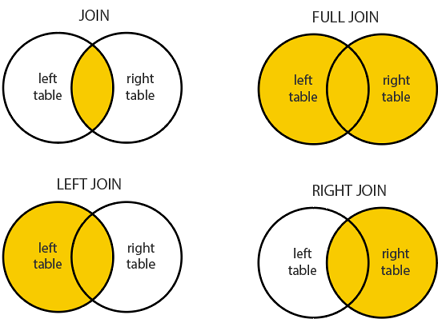
\includegraphics[height=6cm]{joins.png}
	\end{center}
  \caption{The Types of JOINs}
  \label{fig:types of joins}
\end{figure}
\begin{lstlisting}
SELECT column_name(s)
FROM table1
LEFT JOIN table2
ON table1.column_name = table2.column_name;
\end{lstlisting}

\subsection{Normalisierung von Datenbanken}

Unter Normalisierung eines relationalen Datenschemas (Tabellenstruktur) versteht man die Aufteilung von Attributen (Tabellenspalten) in mehrere Relationen (Tabellen) gemäß den Normalisierungsregeln, sodass eine Form entsteht, die keine vermeidbaren Redundanzen mehr enthält.

\subsubsection{1. Normalform}

Eine Relation befindet sich in der ersten Normalform, wenn alle Attribute nur einfache Attributwerte aufweisen (Bezeichnung: atomar)

\subsubsection{2. Normalform}

Eine Relation befindet sich in der zweiten Normalform, wenn sie in der ersten Normalform ist und jedes Nichtschlüsselattribut vom Primärschlüssel voll funktional abhängig ist.

\subsubsection{3. Normalform}

Eine Relation befindet sich in der dritten Normalform, wenn sie in der zweiten Normalform ist und jedes Nichtschlüsselattribut nicht transitiv vom Primärschlüssel abhängig ist, d.h. aus keinem Nichtschlüsselattribut folgt ein anderes Nichtschlüsselattribut.



\subsubsection{Beispiel}

\textbf{Ausgangstabelle}
\begin{table}[H]
    \centering
    \begin{tabular}{|p{0.2\textwidth}|p{0.2\textwidth}|p{0.2\textwidth}|p{0.2\textwidth}|p{0.2\textwidth}|}
    \hline
        CD\textunderscore ID&Album&Gründungsjahr&Erscheinungsjahr&Titelliste \\\hline

        4711&Anastacia – Not That Kind&1999&2000&(1. Not That Kind, 2. I’m Otta Love, 3. Cowboys \& Kisses \\\hline

        4712&Pink Floyd – Wish You Were Here&1965&1975&(1. Shine On You Crazy Diamond) \\\hline

        4713&Anastacia – Freak of Nature&1999&2002&(1. Paid my Dues)
        \\\hline
    \end{tabular}
\end{table}

\textbf{1. Normalform}
\begin{table}[H]
    \centering
    \begin{tabular}{|p{0.1\textwidth}|p{0.1\textwidth}|p{0.1\textwidth}|p{0.2\textwidth}|p{0.2\textwidth}|p{0.1\textwidth}|p{0.1\textwidth}|}
    \hline

        CD\textunderscore ID&Albumtitel&Interpret&Gründungsjahr&Erscheinungsjahr&Track&Titel \\\hline

        4711&Not That Kind&Anastacia&1999&2000&1&Not That Kind \\\hline

        4711&Not That Kind&Anastacia&1999&2000&2&I’m Outta Love \\\hline

        4711&Not That Kind&Anastacia&1999&2000&3&Cowboys \& Kisses \\\hline

        4712&Wish You Were Here&Pink Floyd&1965&1975&1&Shine On You Crazy Diamond \\\hline

        4713&Freak of Nature&Anastacia&1999&2002&1&Paid my Dues
        
    \\\hline
    \end{tabular}
\end{table}


\textbf{2. Normalform}
\begin{table}[H]
    \centering
    \begin{tabular}{|p{0.2\textwidth}|p{0.2\textwidth}|p{0.2\textwidth}|p{0.2\textwidth}|p{0.2\textwidth}|}
    \hline
        CD\textunderscore ID&Albumtitel&Interpret&Gründungsjahr&Erscheinungsjahr \\\hline

        4711&Not That Kind&Anastacia&2000&2000 \\\hline

        4712&Wish You Were Here&Pink Floyd&1975&1975 \\\hline

        4713&Freak of Nature&Anastacia&2002&2001
        
    \\\hline
    \end{tabular}
    \caption{CD}
\end{table}

\begin{table}[H]
    \centering
    \begin{tabular}{|p{0.3\textwidth}|p{0.3\textwidth}|p{0.3\textwidth}|}
    \hline
        CD\textunderscore ID&Track&Titel \\\hline

        4711&1&Not That Kind \\\hline

        4711&2&I’m Outta Love \\\hline

        4711&3&Cowboys \& Kisses \\\hline

        4712&1&Shine On You Crazy Diamond \\\hline

        4713&1&Paid my Dues
        
    \\\hline
    \end{tabular}
    \caption{Lied}
\end{table}

\break
\textbf{3. Normalform}
\begin{table}[H]
    \centering
    \begin{tabular}{|p{0.25\textwidth}|p{0.25\textwidth}|p{0.25\textwidth}|p{0.25\textwidth}|}
    \hline

        CD\textunderscore ID&Albumtitel&Interpret\textunderscore ID&Erscheinungsjahr \\\hline

        4711&Not That Kind&311&2000 \\\hline

        4712&Wish You Were Here&312&1975 \\\hline

        4713&Freak of Nature&311&2001
        
    \\\hline
    \end{tabular}
    \caption{CD}
\end{table}

\begin{table}[H]
    \centering
    \begin{tabular}{|p{0.25\textwidth}|p{0.25\textwidth}|p{0.25\textwidth}|}
    \hline

        Interpret\textunderscore ID&Interpret&Gründungsjahr \\\hline

        311&Anastacia&1999 \\\hline

        312&Pink Floyd&1965
        
    \\\hline
    \end{tabular}
    \caption{Künstler}
\end{table}

\begin{table}[H]
    \centering
    \begin{tabular}{|p{0.25\textwidth}|p{0.25\textwidth}|p{0.25\textwidth}|}
    \hline

        CD\textunderscore ID&Track&Titel \\\hline

       4711&1&Not That Kind \\\hline

       4711&2&I’m Outta Love \\\hline

       4711&3&Cowboys \& Kisses \\\hline

       4712&1&Shine On You Crazy Diamond \\\hline

       4713&1&Paid my Dues
        
    \\\hline
    \end{tabular}
    \caption{Lied}
\end{table}

Anmerkung: Wenn Interpret weltweit eindeutig wäre, wäre der künstliche Schlüssel ‚Interpret\textunderscore ID‘ nicht zwingend notwendig.


\subsection{Rechte- und Benutzerverwaltung - vermutlich nicht ASP1}

Mit Hilfe von SQL können Benutzer und Rechte angelegt und verteilt werden. Ein fein unterteiltes Rechtesystem hilft dabei, die Zugriffsberechtigungen von unterschiedlichen Nutzern zu steuern.

\subsubsection{Anlegen von Benutzern}

\begin{lstlisting}
CREATE USER `bob` identified by `test`
\end{lstlisting}
\begin{itemize}[topsep=-10pt]
    \item Legt einen Benutzer bob mit dem Passwort test an
    \item Benutzer kann von überall her auf die Datenbank zugreifen
\end{itemize}

\vspace{20pt}
\begin{lstlisting}
    CREATE USER `tom` identified by `test` WITH MAX_QUERIES_PER_HOUR 2000 PASSWORD EXPIRE INTERVAL 90 DAY;
\end{lstlisting}
\begin{itemize}[topsep=-10pt]
    \item Legt einen Benutzer tom mit dem Passwort test an
    \item Benutzer kann von überall her auf die Datenbank zugreifen
    \item Maximal 2000 Anfragen pro Stunde
    \item Passwort muss spätestens nach 90 Tagen erneuert werden
\end{itemize}

\subsubsection{Zuweisen von Rechten}
\begin{lstlisting}
    GRANT ALL ON haro02.* TO bob
    FLUSH PRIVILEGES
\end{lstlisting}
\begin{itemize}[topsep=-10pt]
    \item GRANT ALL PRIVILEGES: Alle Verfügbaren Rechte werden vergeben (Rechte können fein granuliert werden \textrightarrow\space \url{https://mariadb.com/kb/en/grant/}
    \item Benutzer kann von überall her auf die Datenbank zugreifen
    \item Maximal 2000 Anfragen pro Stunde
    \item Passwort muss spätestens nach 90 Tagen erneuert werden
\end{itemize}

\subsubsection{Anzeigen aller Benutzer}
\begin{lstlisting}
    SELECT * FROM mysql.user
\end{lstlisting}

\subsubsection{Benutzer löschen}
\begin{lstlisting}
    DROP USER bob
\end{lstlisting}


\subsection{Transaktionsverwaltung - vermutlich nicht ASP1}
Unter einer DB-Transaktion versteht man eine Sammlung von Befehlen, die als logische Einheit verstanden werden.
Entweder sind alle Befehle erfolgreich oder keiner.
Fehlerhafte Transaktionen müssen abgebrochen werden und bisherige Änderungen in der Datenbank rückgängig gemacht werden.

\subsubsection{ACID-Prinzip}
Beim Ausführen einer Transaktion muss das Transaktionssystem die ACID-Eigenschaften garantieren.

\begin{outline}
    \1 Atomarität (Atomicity)
        \2 Transaktion wird entweder ganz oder gar nicht ausgeführt
        \2 Transaktionen sind unteilbar
        \2 Wenn eine atomare Transaktion abgebrochen wird, ist das System unverändert
    \1 Konsistenz (Consisentcy)
        \2 Nach Ausführung einer Transaktion muss der Datenbestand in einer konsistenten Form sein, wenn er es bei Beginn der Transaktion auch schon war
    \1 Isolation (Isolation)
        \2 Bei Ausführung mehrerer Transaktionen gleichzeitig, dürfen diese sich nicht gegenseitig beeinflussen
    \1 Dauerhaftigkeit (Durability)
        \2 Auswirkungen einer Transaktion müssen im Datenbestand dauerhaft bestehen bleiben
        \2 Effekte von Transaktionen dürfen nicht verloren gehen oder verblassen
        \2 Verschachtelung von Transaktionen ist daher streng genommen nicht möglich, da ein Zurücksetzen (Rollback) der äußeren Transaktion die Dauerhaftigkeit der inneren, bereits ausgeführten, Transaktion verletzen würde
\end{outline}

\subsubsection{Ausführen von Transaktionen}

Transaktionen werden durch die Markierungen \textbf{START TRANSACTION} und \textbf{END OF TRANSACTION} (oder \textbf{COMMIT}) abgegrenzt:

\begin{lstlisting}
    START OF TRANSACTION
    WRITE x
    WRITE y
    COMMIT
\end{lstlisting}

\subsubsection{Beenden von Transaktionen}

\begin{enumerate}
    \item Commit: Die Transaktion wurde erfolgreich und ohne Probleme beendet. Die Auswirkungen der Transaktion auf den Datenbestand sind dauerhaft gespeichert.
    
    Oft werden „COMMIT“ und „END OF TRANSACTION“ synonym verwendet
    \item Rollback: Bei der Ausführung sind Probleme aufgetreten und die Ausführung wird nicht fortgesetzt. Sämtliche Auswirkungen auf den Datenbestand müssen rückgängig gemacht werden (Atomarität).
\end{enumerate}

\subsubsection{Autocommit}

Standardmäßig befindet sich MariaDB im Modus Autocommit. Das bedeutet, dass alle Data Manipulation Befehle direkt persistiert werden.

Autocommit beenden: SET AUTOCOMMIT = 0; dann müssen alle Änderungen am Datenbestand mit COMMIT explizit permanent gespeichert werden.
Mit ROLLBACK werden alle Änderungen bis zum letzten Commit rückgängig gemacht.

Autocommit aktivieren: SET AUTOCOMMIT = 1

\pagebreak
\section{ITS Mertens}

\subsection{Datensicherheit}

Datensicherheit hat generell mit der Sicherheit von Daten zu tun. \\
Ziel der Datensicherheit ist der Schutz von Daten allgemein, nicht nur von personenbezogenen Daten. \\
Das oberste Ziel der Datensicherheit besteht in der Gewährleistung der

\begin{itemize}

\item Vertraulichkeit
\item Integrität und
\item Verfügbarkeit von Daten

\end{itemize}
Datensicherheit handelt sich hier um die praktischen Sicherheitsmaßnahmen oder Ansätze zum Schutz von Daten (z.B. Maßnahmen zur Datensicherung, technischer Schutz vor Datenverlust usw.).


\subsection{Datenschutz}

Unter Datenschutz versteht man den Schutz von personenbezogenen Daten. \\
Ziel des Datenschutzes ist der Schutz des allgemeinen Persönlichkeitsrechts der betroffenen Personen. \\
\begin{itemize}

\item Schützen der Grundrechte und Grundfreiheiten einer Person.

\end{itemize}

\subsection{BSI (Bundesamt für Sicherheit in der Informationstechnik)}

Im BSI Grundschutzkompendium kann nachgeschlagen werden:
\begin{itemize}
\item welche möglichen Gefährdungen bestehen
\item welche Auswirkungen diese haben
\item wie ein Unternehmen sich dagegen schützen kann
\end{itemize} 
Das BSI Grundschutzkompendium ist bei einer Schutzbedarfsanalyse als Nachschlagewerk zu betrachten, jedoch nicht als abgeschlossene Analyse, da diese für jedes Unternehmen unterschiedlich ist.

\subsection{Schutzbedarfskategorien}

\begin{itemize} 
\item normal: Begrenzte und überschaubare Auswirkungen \\
\item hoch: Beträchtliche Auswirkungen \\
\item sehr hoch: Kritische, möglicherweise existenzbedrohende Auswirkungen
\end{itemize}

\subsection{Schadensszenarien}

\begin{itemize}
\item Verstöße gegen Gesetze, Vorschriften oder Verträge
\item Beeinträchtigungen des informationellen Selbstbestimmungsrechts
\item Beeinträchtigungen der persönlichen Unversehrtheit
\item Beeinträchtigungen der Aufgabenerfüllung
\item Negative Innen- oder Außenwirkung
\item Finanzielle Auswirkungen
\end{itemize}

\subsection{Schutzziele}

\paragraph{Vertraulichkeit}
Schutz vor Verrat von Informationen oder vertraulichen Daten. \\
Darunter sind z.B. Umsatzzahlen und daraus erhobene Daten oder Produkt- und Forschungsergebnisse zu verstehen. \\
(Interessant für die Konkurrenz) 
\begin{itemize}
\item[=] Vertrauliche Informationen unberechtigt zur Kenntnis genommen oder weitergegeben
\end{itemize}
\paragraph{Integrität}
Das durchgängige Funktionieren von IT-Systemen sowie die Vollständigkeit und Richtigkeit von Daten und Informationen.\\ In Bezug auf die Informationssicherheit bedeutet Integrität das Verhindern von nicht genehmigten Veränderungen an wichtigen Informationen. \\
Integrität von Daten kann man z.B. durch Verschlüsselung erreichen. 

\begin{itemize}
\item[=] Die Korrektheit der Informationen und der Funktionsweise von Systemen ist nicht mehr gegeben
\end{itemize}
\paragraph{Verfügbarkeit  von Daten}
Definiert, zu welchem Grad IT-Systeme, IT Anwendungen, IT Netzwerke und elektronische Informationen einem Benutzer zur Verfügung stehen und ohne Einschränkung verwendet werden können.

\begin{itemize}
\item[=] Autorisierte Benutzer werden am Zugriff auf Informationen und Systeme behindert
\end{itemize}

\subsection{DSGVO - Datenschutz-Grundverordnung}

Die EU-Datenschutzgrundverordnung (DSGVO) ist unmittelbar geltendes Recht. Sie hat Vorrang vor nationalem Recht. An manchen Stellen lässt sie aber einzelne Bestimmungen offen (Öffnungsklauseln). Diese werden durch das Bundesdatenschutzgesetz (BDSG) konkretisiert.

\subsection{Grundsätze der DSGVO}

\textbf{Rechtmäßigkeit}, Verarbeitung nach Treu und Glauben, Transparenz
Personenbezogenen Daten dürfen nur so verarbeitet werden, wie es bei der Erhebung angegeben wurde. Zudem muss die Verarbeitung in einer für den Betroffenen nachvollziehbaren Weise erfolgen. Es sind keine verdeckte oder geheime Verarbeitung erlaubt. Die betroffene Person sollte wissen, wer der Verantwortliche für die Verarbeitung ist.

\textbf{Zweckbindung}
Personenbezogene Daten dürfen nur für den Zweck verarbeitet werden, für den sie erhoben wurden.
Beispiel:
Ein Kunde widerruft seine Einwilligung zum Erhalt von Newslettern. Ab diesem Zeitpunkt ist der Zweck der Datenverarbeitung nicht mehr gegeben. Somit darf das Unternehmen die Daten der betroffenen Person nicht mehr verarbeiten.

\textbf{Datenminimierung}
Unternehmen dürfen nur so viele Daten erheben und verarbeiten, wie sie tatsächlich benötigt. Die Daten müssen für den Zweck erheblich und relevant sein. 
Beispiel: 
Für den Abschluss eines Kaufvertrages darf die Religionszugehörigkeit oder der Familienstand nicht zusätzlich erhoben werden. Denn diese spielen für den Kauf keine wesentliche Rolle.

\textbf{Richtigkeit} 
	Daten müssen inhaltlich und sachlich richtig und aktuell gehalten werden.

\textbf{Speicherbegrenzung} 
Speicherbegrenzung bezieht sich auf die Dauer der Speicherung. Daten dürfen nicht für die Ewigkeit gespeichert werden. Ist der Zweck nicht mehr gegeben, müssen die Daten gelöscht werden.
	
\textbf{Integrität und Vertraulichkeit} 
Die Daten müssen vor unrechtmäßiger Verarbeitung durch Unbefugte geschützt werden. Ebenso müssen die Daten vor versehentlicher Beschädigung oder Verlust geschützt werden.

\textbf{Rechenschaftspflicht}
In der DSGVO gilt die Rechenschaftspflicht, d.h. die verantwortliche Stelle ist für die Einhaltung der oben genannten Grundsätze verantwortlich. Auf Verlangen muss sie die Einhaltung gegenüber den Betroffenen und den Behörden nachweisen können.

\subsection{Schutzbedarfsanalyse}

Sicherheitskonzept, das drei Schutzzielen, deren potenziellen Gefährdungen und die Auswirkungen / Maßnahmen dagegen dokumentiert. \\
\\
\textbf{Verlust der Verfügbarkeit von Informationen} \\
\textbf{Gefährdung}: Verschleiß von Festplatten, die Daten speichern.\\
\textbf{Auswirkungen}: Totaler Ausfall \\ (die Daten werden für den laufenden Geschäftsbetrieb dauerhaft benötigt) \\
\textbf{Maßnahmen dagegen}: 
\begin{itemize}
\item Daten auf mehreren Festplatten speichern (RAID)
\item Festplatten regelmäßig überprüfen und ggf. austauschen
\item Daten in verschiedenen Rechenzentren speichern und aktuell halten
\end{itemize}
\vspace{1cm}
\textbf{Verlust der Vertraulichkeit von Informationen} \\
\textbf{Gefährdung}: Sicherheitslücke in einem Rechenzentrum \\
\textbf{Auswirkungen}: Fremde können sich Zugang zu den Servern beschaffen und Daten abgreifen. \\
Verschlechtert das Ansehen des Unternehmens, ggf. rechtliche Konsequenzen \\
\textbf{Maßnahmen dagegen}: 
\begin{itemize}
\item Daten nur verschlüsselt speichern
\item Eigene Rechenzentren verwenden, um die maximale Kontrolle über Sicherheitsaspekte zu haben
\item Regelmäßig Sicherheitstests (auch extern)
\item Zugang zu Servern beschränken
\item Daten verschieden lagern um Schaden zu begrenzen
\end{itemize}
\vspace{1cm}
\textbf{Verlust der Integrität} \\
\textbf{Gefährdung}: Sicherheitslücke in einem Rechenzentrum \\
\textbf{Auswirkungen}: Unbefugter Zugang zu Servern Manipulation von Daten \\
Fehlerhafte Daten und damit ungewolltes Verhalten der Software \\
\textbf{Maßnahmen dagegen}: 
\begin{itemize}
\item Daten nur verschlüsselt speichern
\item Eigene Rechenzentren verwenden, um die maximale Kontrolle über Sicherheitsaspekte zu haben
\item Regelmäßig Sicherheitstests (auch extern)
\item Zugang zu Servern beschränken
\item Daten verschieden lagern um Schaden zu begrenzen
\item RAID-Backups
\end{itemize}
\vspace{1cm}

\subsection{Urheberrecht}

Das Urheberrecht schützt den Urheber in seinen geistigen, persönlichen und vermögensrechtlichen Beziehungen zu seinem Werk, dessen Rechtsschutz mit seiner Entstehung beginnt und im Unterschied zu den gewerblichen Schutzrechten keiner Hinterlegung oder Registrierung bedarf. Als dem Urheberrecht zugängliche Werkarten nennt das UrhG Sprachwerke (Reden, Schriftwerke und Computerprogramme), Werke der Musik, pantomimische Werke und Werke der Tanzkunst, Werke der bildenden und angewandten Kunst, Bauwerke, Lichtbildwerke, Filmwerke sowie Darstellungen wissenschaftlicher und technischer Art (Zeichnungen, Pläne, Karten, Skizzen, Tabellen, plastische Darstellungen).

Neben dem Urheberrecht spielt auch das Markenrecht eine Rolle. Für die Benutzung geschützter Werke benötigt man im geschäftlichen Umfeld in der Regel eine Lizenz. 

\subsection{SLA - Service Level Agreement}

Ein SLA ist ein Vertrag zwischen einem Dienstleistungsanbieter und seinen Kunden. \\
Dieser dokumentiert welche Dienstleistungen der Anbieter erbringen wird. \\
Zudem definiert er Dienstleistungsstandards, zu deren Einhaltung der Anbieter verpflichtet ist. 

Beinhaltet z.B.:
\begin{itemize}

\item die Verfügbarkeit
\item[] Beispiel: $99,7\%$ Verfügbarkeit 
\begin{enumerate}
\item $365 * 24 * (100-99,7)$  =  Maximale Downtime
\item Reaktionszeit beachten
\item Frage: Ist die Zeit überschritten?
\item Frage: Ist die max. Entstördauer überschritten
\end{enumerate}
\item Servicebereitschaft von wann bis wann
\item Reaktionszeit auf Störungen und maximale Entstördauer
\item Ggf. Hinweise zum Monitoring von Produkten

\end{itemize}

\subsubsection{First Level Support}

Dieser ist der Erste Ansprechpartner für Beratung und Hilfe im IT- und Computerbereich. \\
Wird er kontaktiert, trägt er zunächst die Daten des Kunden, alle eingehenden Anfragen und weitergehende Informationen zusammen. \\ 
Anschließend listet er sie auf. \\
Die Dokumentation sollte möglichst lückenlos erfolgen. \\
Dies verhindert unangenehme Nachfragen des Kunden und gewährleistet eine reibungslose Weitergabe der Anfrage an den nächsten Support-Level.  \\
Zunächst kümmert sich aber der First-Level-Supporter eigenständig um das Problem. \\
Neben seiner Erfahrung kann er bei Bedarf auch das Wissen externer Datenbanken zu Rate ziehen. \\
In dieser Phase erfolgt daneben auch eine Einstufung der Probleme, die die Kunden haben.

\subsubsection{Second Level Support}

Dieser ist die zweite Ebene im Kundenservice eines Unternehmens. \\
Er versucht technischer Probleme beim Kunden per Ferndiagnose am Telefon oder per Internet-Online Support zeitnah zu lösen. \\
Second Level Supporter müssen über entsprechendes Fachwissen verfügen, das beim First Level Support nicht zwingend erforderlich ist.


\subsubsection{Third Level Support}

Dieser besteht ausschließlich aus Experten und Spezialisten. \\ 
Diese Stufe wird nur eskaliert, wenn der Second Level keine Lösung gefunden hat.


\subsection{ITIL  (Information Technology Infrastructure Library)}

Der \textbf{ITIL}  ist der \textbf{Best-Practice-Leitfaden} und der \textbf{De-facto-Standard} im Bereich IT-Service-Management. \\
Er besteht nicht aus starren Vorgaben, sondern ist vielmehr eine Sammlung von Leitlinien, die an die Anforderungen einzelner Unternehmen angepasst werden können.
\subsection{Kategorisierung}
\subsubsection{Service Request}

\textbf{Service Requests} sind formale Anfragen eines Anwenders nach etwas, das bereitgestellt werden soll. \\
\begin{itemize}
\item Anfrage nach Informationen
\item Beratung 
\item Passwort zurücksetzen
\item Arbeitsplatz für einen neuen Anwender aufsetzen
\end{itemize}

\subsubsection{Event}
\textbf{Events} sind einfache Benachrichtigungen, die keinen Fehler darstellen müssen \\
\begin{itemize}
\item Statusänderung 
\item Alarm 
\item Benachrichtigung
\end{itemize}

\subsubsection{Incident}
Ein Incident ist eine Beeinträchtigung oder Unterbrechung eines angebotenen Service. \\
Eine Beeinträchtigung liegt dann vor, wenn der Service nach der Vereinbarung zwischen Servicegeber und Servicenehmer (SLA) quantitativ oder qualitativ nicht wie vereinbart genutzt werden kann.

\section{BWL}
\subsection{Unternehmensphilosophie}
Grundelemente einer Unternehmensphilosophie sind die 
\begin{itemize}
\item Grundwerte und Überzeugungen 
\item Standards und Symbole des  Unternehmens
\end{itemize}
Es ist der `Charakter` des  Betriebs. \\
Es ist  wichtig, dass Angestellte hinter dieser Philosophie stehen. \\
Ein Unternehmensleitbild beinhaltet oft:
\begin{itemize}
\item Wie verhalten wir uns gegenüber Kunden etc.
\item Was macht uns aus? (Standards \& Symbole)
\end{itemize}

\subsection{Unternehmensleitbild} 
Man kann es als `Richtschnur des alltäglichen Handelns` sehen. \\
Wird das Leitbild nicht befolgt, so schadet das Leitbild dem Unternehmen.
Es legt fest:
\begin{itemize}
\item Grundlegende Zwecke
\item Zielrichtungen
\item Strategie
\end{itemize}

\break

\subsection{Unternehmensziele}
Diese leiten sich aus dem Leitbild ab. \\
Man unterscheidet diese Ziele in:
\begin{itemize}
\item \textbf{Ökonomisches} Ziel (Wirtschaftlicher Erfolg)
\item \textbf{Soziales} Ziel (Guter Ruf intern/extern)
\item \textbf{Ökologisches} Ziel (Umwelt helfen)
\end{itemize}
Verschiedene Ziele können im Konflikt, in Harmonie oder in Indifferenz zueinander sein.  \\
\begin{itemize}
\item \textbf{Konkurrierende Ziele}: Ein Ziel verhindert/erschwert das Erreichen des Anderen.
\item \textbf{Komplementäre Ziele}: Ein Ziel fördert gleichzeitig ein anderes.
\item \textbf{Indifferente Ziele}: Das Ziel beeinflusst ein anderes Ziel nicht.
\end{itemize}

\subsubsection{Ökonomische Ziele}
Ein Ökonomisches Ziel kann 3 Kategorien angehören: \\
\begin{enumerate}
\item \textbf{Marktziele}: Stellung, die ein Unternehmen auf dem Markt will
\item \textbf{Ertragsziele}: Alles, das mit Profiterhöhung zu tun hat.
\item \textbf{Leistungsziele}: Streben  nach hoher Qualität, Verpflichtungen gegen Familientraditionen etc. \\
\end{enumerate}
Ihnen liegt das Ökonomische Prinzip zugrunde. \\
Dieses besagt: \\
\begin{itemize}
\item \textbf{Maximalprinzip}: größter  Profit mit gegebenem Kapital
\item \textbf{Minimalprinzip}: Einen Erfolg so wenig wie möglich benötigten Mitteln erreichen
\end{itemize}

\subsubsection{Ökologische Ziele}
Hier geht es darum nicht mehr nach dem Prinzip `Wer Schaden verursacht muss ihn beseitigen` sondern darum, dass dieser Schaden in erster Linie nicht entsteht.

\subsubsection{Soziale Ziele}
Hier stellt das Unternehmen seine Mitarbeiter und seine Kunden in den Mittelpunkt. \\
Bsp.:
\begin{itemize}
\item Urlaubsgeld
\item Zuschüsse  Kantine
\item Familienzulage
\item Altersabsicherung
\item Fördern geistiger und sportlicher Seite \& der Interessen
\end{itemize}
Nebenziele der Sozialen Ziele könnten
\begin{itemize}
\item Arbeitnehmerbindung
\item Steigerung der Arbeit
\item Mehr Einfluss auf die Arbeitnehmer
\end{itemize}
sein.

\subsection{Corporate Identity}
Die Corporate Identity ist die Erscheinungsformen eines Unternehmens nach Außen. \\
Es dient dazu, dass sich Menschen mit dem Unternehmen identifizieren können. \\
Es wird genutzt um ein Unternehmensleitbild abzuleiten. \\
Es wird in 3 Teilbereiche unterschieden:
\begin{enumerate}
\item \textbf{Corporate Design}: Wiedererkennung durch:
\begin{enumerate}
\item Einheitliche Designs (Logo)
\item Farbschemas
\item akustische Elemente
\end{enumerate}
\item \textbf{Corporate Behaviour}: Das Verhalten des Unternehmens und der Mitarbeiter  gegenüber Externen und Internen.
\item \textbf{Corporate Communication}: Einheitliche Kommunikation des Unternehmens (nicht eine Abteilung umweltfreundlich und die andere gezielt schädigend)
\end{enumerate}

\subsection{Wichtige Begriffe}
\subsubsection{Handelsregister}
Öffentliches Verzeichnis aller Kaufleute nach HGB des Amtsgerichtsbezirks. \\
Es erteilt Auskünfte über:
\begin{itemize}
\item Firma
\item Rechtsform
\item Inhaber / persönlich haftende Gesellschafter
\item Wechsel der Inhaber / Gesellschafter
\item Ort der Niederlassung
\item Betrag der Kommanditeinlage
\item Eröffnung der Insolvenz
\item Löschung der Firma
\end{itemize}

\subsubsection{Handelsregister Abteilung A (HRA)}
Hier befinden sich:
\begin{itemize}
\item Einzelunternehmen
\item Personengesellschaften
\item  rechtsfähige wirtschaftliche Vereine
\end{itemize}

\subsubsection{Handelsregister Abteilung B (HRB)}
Hier befinden sich  Kapitalgesellschaften.

\subsection{Firma}
Die Firma eines Kaufmanns ist der Name, unter dem er seine Geschäfte betreibt und die Unterschrift abgibt.

\subsubsection{Firmenzusatz}
Der Firmenzusatz zeigt die Rechtsform des Unternehmens und daher welche Regeln und Vorschriften gelten. \\
Verschiedene Formen:
\begin{itemize}
\item GmbH
\item AG
\item Inc.
\item Corp.
\item Ltd.
\end{itemize}

\subsubsection{Arten der Namen von Firmen}
Man unterscheidet Firmen in ihrer Namensherkunft:
\begin{itemize}
\item \textbf{Personenfirma}: Benannt nach einer Person
\item \textbf{Sachfirma}: Benannt nach einem Zweck
\item \textbf{Fantasiefirma}: Nach einem Fantasienamen benannt
\item \textbf{Mischfirma}: Kombination der anderen Firmenarten
\end{itemize}

\subsubsection{Firmenarten}
Es gibt verschiedene Arten von Firmen. \\
Diese Unterscheiden sich in einer Vielzahl von Punkten: \\ \\

\begin{itemize}
\item \textbf{GmbH}: Gesellschaft mit beschr\"ankter Haftung
\item \textbf{UG}: Unternehmergesellschaft
\item \textbf{AG}: Aktiengesellschaft
\item \textbf{OHG}: Offene Handelsgesellschaft
\item \textbf{KG}: Kommanditgesellschaft
\item[]
\item vollhaftender = Komplement\"ar
\item teilhaftender = Kommanditist
\end{itemize}

\begin{figure}[H]
\begin{center}
  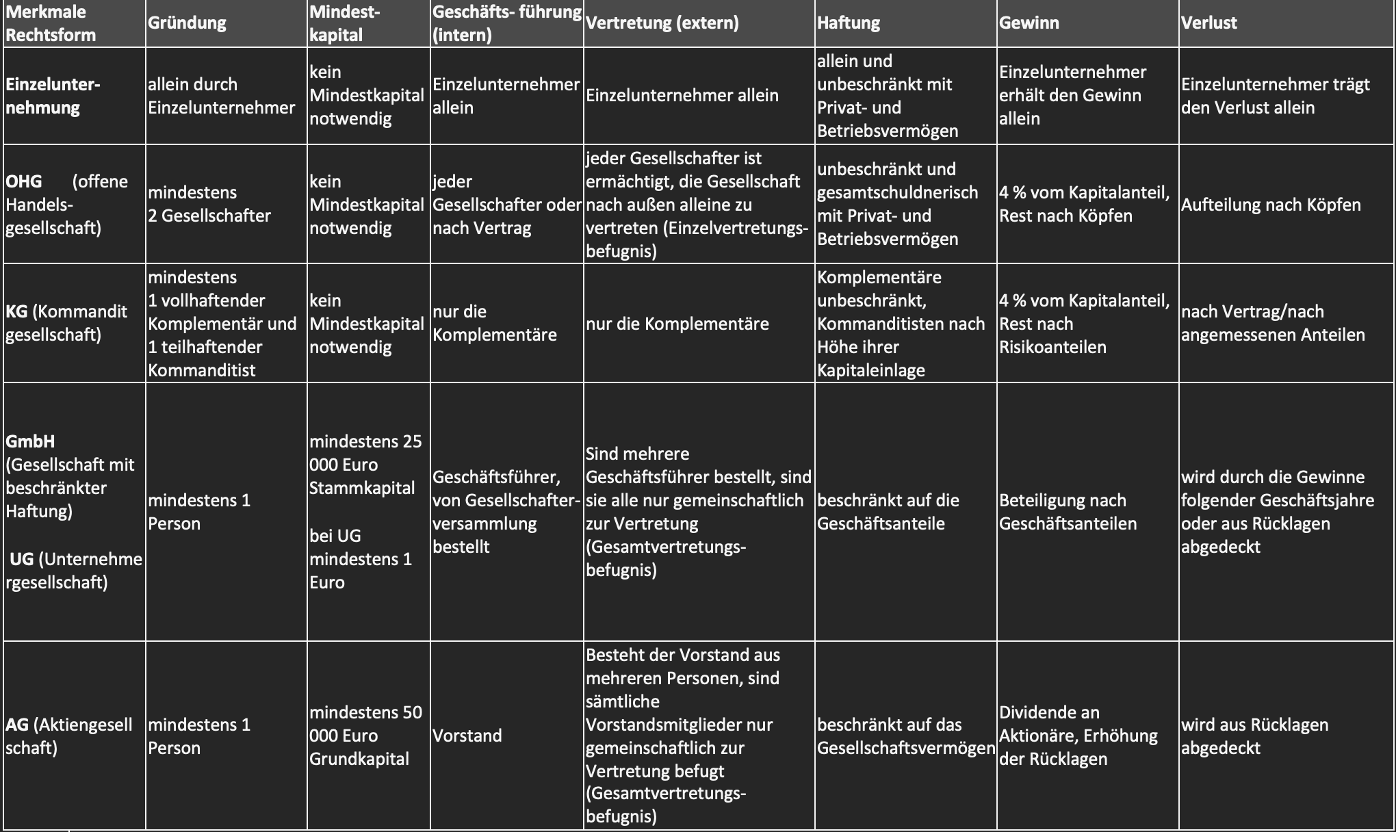
\includegraphics[height=9cm]{arten.png}
\end{center}
  \caption{Arten von Firmen}
  \label{fig: Arten von Firmen}
\end{figure}

\subsubsection{Firmengrundsätze}
Firmen müssen folgende Grundsätze einhalten: 
\begin{enumerate}
\item \textbf{Firmenwahrheit und Firmenklarheit}: Die Firma darf nicht irreführend,  sprich klar und eindeutig sein. Es dürfen beim Kunden keine falschen Erwartungen entstehen.
\item \textbf{Offenlegung der Gesellschaftsverhältnisse}: Diese Offenlegung beinhaltet Infos über Gesellschafter und Eigentümer als auch deren Anteile.
\item \textbf{Offenlegung der Haftungsverhältnisse durch Rechtsformzusatz}: Eine Firma muss ihren Haftungsstatus klarstellen. Dies geschieht durch den Zusatz zur Firmenbezeichnung.
\item \textbf{Firmenbeständigkeit}: Hier geht es darum, dass  der Name der nicht zu  oft wechseln darf und nur mit Begründung.
\item \textbf{Firmenöffentlichkeit}:  Jedes Unternehmen muss im Handelsregister eingetragen sein. 
\item \textbf{Firmenausschließlichkeit}: Der Name einer Firma muss sich von den Namen aller anderen Firmen unterscheiden.
\item \textbf{Firmengeheimnis}: Bestimmte Informationen dürfen geheim gehalten werden um wettbewerbsfähig zu bleiben.
\item \textbf{Firmenfortführung}: Wird das Unternehmen  verkauft/in eine  andere Rechtsform umgewandelt, so bleibt die Bezeichnung i.d.R gleich. \\
Dies soll das Vertrauen der Kunden und Geschäftspartner in das Unternehmen erhalten.
\item \textbf{Firmenlöschung}: Wenn ein Unternehmen aufgelöst oder liquidiert wird, muss die Firmenbezeichnung aus dem Handelsregister gelöscht werden. \\
Dies bedeutet, dass die Firma nicht mehr aktiv ist und keine Geschäfte mehr tätigt. 
\end{enumerate}

\subsubsection{Grundfunktionsbereiche}

\begin{figure}[H]
\begin{center}
  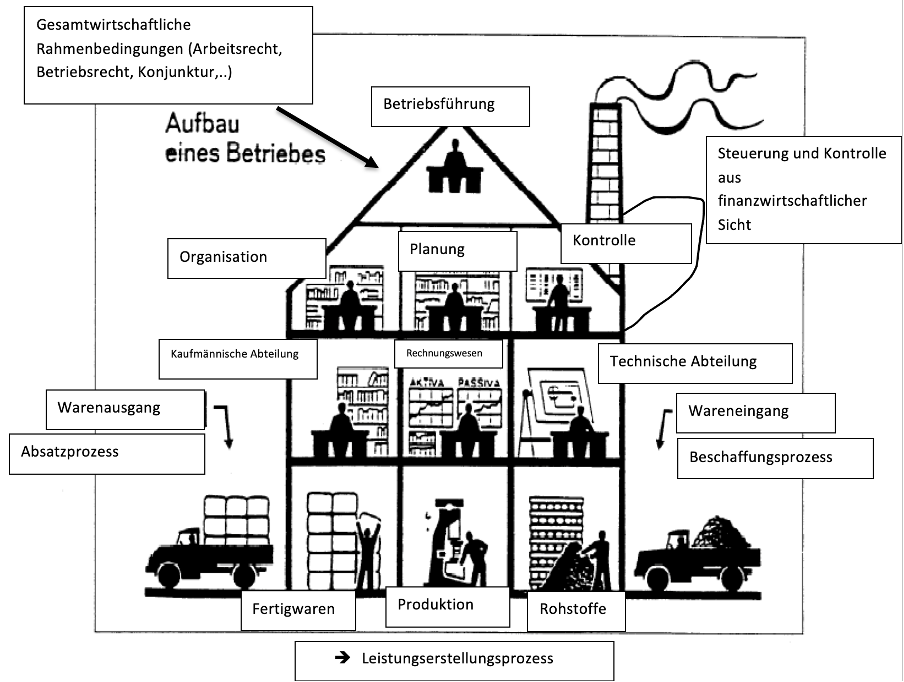
\includegraphics[height=6cm]{funktionsbereiche_firma.png}
  \end{center}
  \caption{Grundfunktionsbereiche von Firmen}
  \label{fig: Grundfunktionsbereiche von Firmen}
\end{figure}
Als Grundfunktionsbereich bezeichnet man Bereiche, die für Industriebetriebe charakteristisch/unverzichtbar sind. \\
Es wird in die folgenden Grundfunktionsbereiche unterschieden:
\begin{itemize}
\item \textbf{Materialwirtschaft}: Beschaffung, Verwaltung von  Materialien
\item \textbf{Produktionswirtschaft}: Organisiert die Fertigung
\item \textbf{Absatzwirtschaft}: Dreht sich um den Verkauf des Produzierten
\end{itemize}

\subsubsection{Unterstützungsfunktionsbereiche}
Neben den Grundfunktionsbereichen gibt es noch die Unterstützungsfunktionsbereiche. \\
Diese sind dafür verantwortlich, dass die Grundfunktionsbereiche reibungslos ablaufen können. \\
Zu ihnen gehören:
\begin{itemize}
\item \textbf{Finanzwirtschaft}: Dieser wird nochmal unterteilt in:
\begin{itemize}
\item \textbf{Finanzierung}: Bezeichnet die Bereitstellung finanzieller  Mittel.  
\item \textbf{Investition}: Bezeichnet die Verwendung finanzieller Mittel (größere  Beiträge, Kapitalbindung)
\end{itemize}
\item \textbf{Personalwirtschaft}: Beschäftigt sich mit Anzahl und Qualifikationen des Personals
\item \textbf{Rechnungswesen}: Erfassung des  betrieblichen Prozesses eines Unternehmens. \\
Man unterscheidet in:
\begin{itemize}
\item \textbf{Internes Rechnungswesen}:
\begin{itemize}
\item Kosten- und Leistungsrechnung
\item Betriebsstatistik 
\item Planungsrechnung
\end{itemize}
\item \textbf{Externes Rechnungswesen}:
\begin{itemize}
\item Buchführung
\item Jahresabschlussrechnung
\end{itemize}
\end{itemize}
\item \textbf{Controlling}: Das Controlling unterstützt die Geschäftsleitung indem es:
\begin{itemize}
\item Informationen beschafft \& aufbereitet
\item das Unternehmen mitsteuert, koordiniert und analysiert
\end{itemize} 
\end{itemize}

\subsubsection{Querschnittsfunktion}
Die Unterstützungsfunktionsbereiche haben eine Querschnittsfunktion. \\
Diese besagt, dass die einzelnen Unterstützungsfunktionsbereiche jeweils allen Grundfunktionsbereichen zuarbeiten. \\
So regelt beispielsweise die Personalwirtschaft im Einvernehmen mit der Geschäftsleitung jeweils alle Personalentscheidungen, also sowohl in der Absatz- wie in der Produktions- oder Materialwirtschaft.

\begin{figure}[H]
\begin{center}
  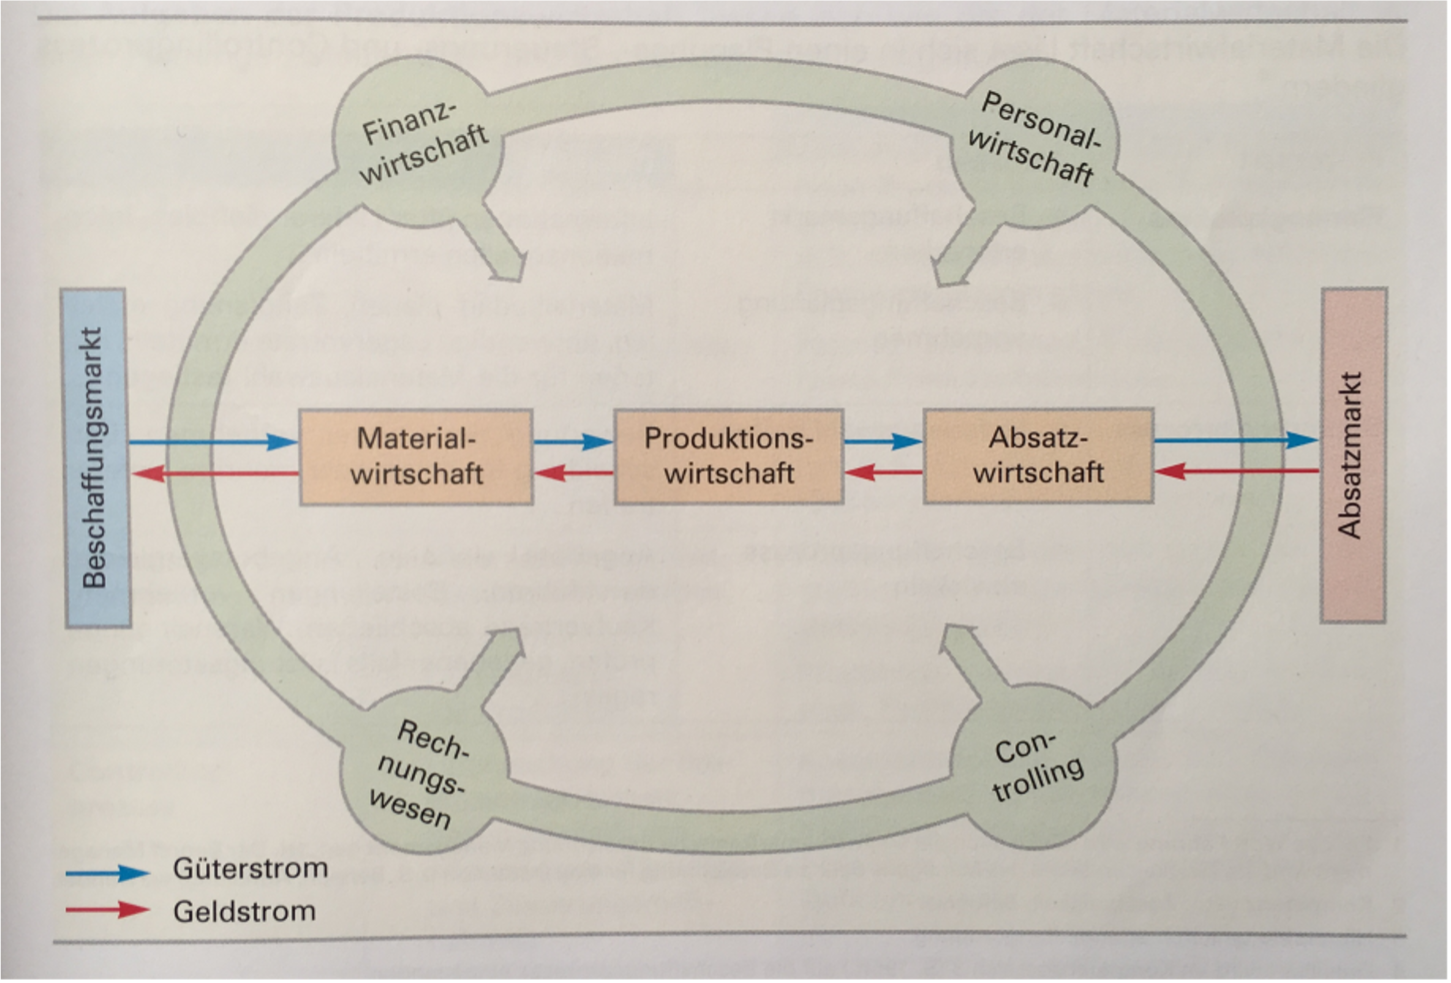
\includegraphics[height=6cm]{querschnitt.png}
  \end{center}
  \caption{Die Querschnittsfunktion}
  \label{fig: Die Querschnittsfunktion}
\end{figure}

\subsection{Prokura}
Eine Prokura ist eine Vollmacht, die eine Person oder mehrere Personen ermächtigt, im Namen eines Unternehmens oder einer Organisation rechtsgültige Entscheidungen zu treffen und Verträge abzuschließen. \\
Der Prokurist ist ein kaufmännischer Angestellter, dessen Wirkungsbereich im Interesse der Rechtssicherheit nach außen durch eine typisierte Vertretungsmacht festgelegt ist. \\ \\
Die Eintragung erfolgt durch den Kaufmann und nur mit ausdrücklicher Erklärung. \\
Eine deklaratorische HR-Eintragung ist notwendig. \\
Eine  Prokura ist im  Innenverhältnis mit Ernennung gültig, im Außenverhältnis erst  nach HR-Eintragung und Mitteilung an Dritte. \\
Der Umfang der Prokura kann nach \textbf{außen}  nicht beschränkt werden. \\ \\

\break

Beendet  wird  die  Prokura durch:
\begin{itemize}
\item Auflösung des Arbeitsvertrages
\item Widerruf
\item Geschäftsauflösung
\item Tod des Prokuristen
\item \textbf{Nicht}  bei Tod des Geschäftsinhabers
\item Bei Inhaberwechsel, wenn der neue Inhaber dies will
\end{itemize}


\subsubsection{Varianten}
\begin{itemize}
\item \textbf{Einzelprokura}: Es gibt nur 1  Prokurist (höchste Prokura).
\item \textbf{Filialprokura}: Prokurist hat nur über 1 Niederlassung Befugnisse.
\item \textbf{Gesamtprokura}: Bestimmt mehrere Prokuristen (niedrigste Prokura)
\end{itemize}

\begin{figure}[H]
\begin{center}
  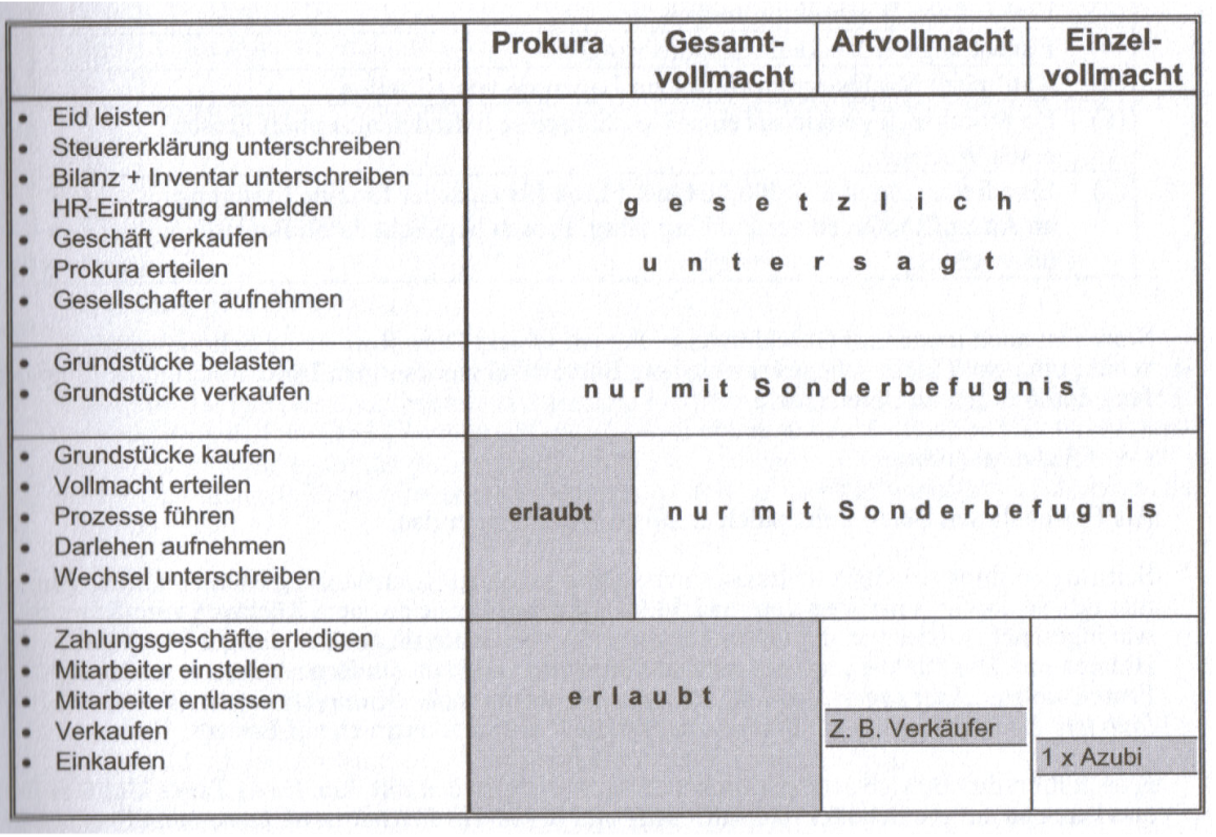
\includegraphics[height=6cm]{prokura.png}
  \end{center}
  \caption{Rechte der Prokuristen}
  \label{fig:Rechte der Prokuristen}
\end{figure}

\subsection{Handlungsvollmacht}
Es gibt verschiedene Varianten:
\begin{itemize}
\item \textbf{Allgemeine Handlungsvollmacht}: Erlaubt, alle üblichen Aufgaben des Geschäftszweigs zu tätigen. Man unterscheidet ob mit Sondervollmacht oder ohne.
\item \textbf{Artvollmacht}: Wahrnehmung begrenzter, sich wiederholender Aufgaben gleicher Art
\item \textbf{Einzelvollmacht}:  Wahrnehmung einzelner Aufgaben
\end{itemize}
Die  Erteilung einer  Handlungsvollmacht  erfolgt durch:
\begin{itemize}
\item den Kaufmann
\item den Prokuristen
\item einen weitgehend bevollmächtigten (`Untervollmachten`)
\item Formlos
\item Keine Eintragung notwendig
\end{itemize}
Sie kann widerrufen werden durch:
\begin{itemize}
\item Widerruf
\item Kündigung des Arbeitsvertrages
\item Geschäftsauflösung
\item Inhaberwechsel, wenn der Inhaber widerruft
\item Einzelvollmacht
\end{itemize}

\subsection{Kaufmann}
Ein Kaufmann ist, nach dem Handelsgesetzbuch (HGB) der, der ein Handelsgewerbe betreibt. \\
Ein Handelsgewebe ist ein Gewerbe mit einer Kaufmännischen Organisation\\
(Eine Firma die Umsatz, Gewinn macht, Mitarbeiter hat, EDV-Anlagen == Firma die was verkauft) \\
Kaufmänner können unterschieden werden in:
\begin{itemize}
\item Ist-Kaufmann
\item Kann-Kaufmann
\item Form-Kaufmann
\end{itemize}

\subsubsection{Ist-Kaufmann}
Ist-Kaufmann ist, wer ein Handelsgewerbe betreibt, das nach Art und Umfang einen kaufmännisch geführten Geschäftsbetrieb erfordert. \\
Der Inhaber eines solchen Geschäftsbetriebes ist kraft Gesetzes Kaufmann (Ist-Kaufmann). \\
Er muss sich in das Handelsregister eintragen lassen, ist jedoch schon vor Eintragung Kaufmann.

\subsubsection{Kann-Kaufmann}
Ein Kann-Kaufmann ist ein Kaufmann eines Kleingewerbes, der nicht im Handelsgesetzbuch eingetragen und somit nicht auf rechtlicher Grundlage ein Kaufmann ist. \\
Er wird zum Kaufmann im Sinne des HGB, sobald er im Handelsgesetzbuch eingetragen ist. \\ \\
Für Land und Forstwirtschaft gibt es hier eine Ausnahme: \\
Land und Forstwirtschaftliche Gewerbe mit einer kaufmännischen Einrichtung haben das Recht zur Eintragung. \\
Dadurch können sie zum kann-Kaufmann werden. \\
Ohne die kaufmännischen Organisation haben sie dieses Recht nicht und sind dadurch Nicht-Kaufmann.

\subsubsection{Form-Kaufmann}
Ein Formkaufmann besitzt die Kaufmannseigenschaft kraft seiner Rechtsform. \\
(z.b. GmbH, OHG, KG, etc.)

\subsection{Leitungssysteme}
Auch Weisungssysteme genannt. \\
Sie betrachten die Unternehmensstruktur unter dem Aspekt \"Uber- und Unterordnung (Weisungsbefugnis)

\subsubsection{Einliniensystem}
Kennzeichen: \\
\begin{itemize}
\item Alle Mitarbeiter sind einer strengen Hierarchie gebunden
\item Anweisungen erhält man immer von der Stelle unmittelbar \"uber der Eigenen
\item Meldungen und Berichte gehen genauso nur an die Stelle darüber
\item Nur dieser eine vertikale Dienstweg ist vorhanden und muss eingehalten werden
\item Kontakte zu gleichrangigen Stellen führen zwingend über die gemeinsame übergeordnete Stelle
\end{itemize}
\begin{figure}[H]
\begin{center}
  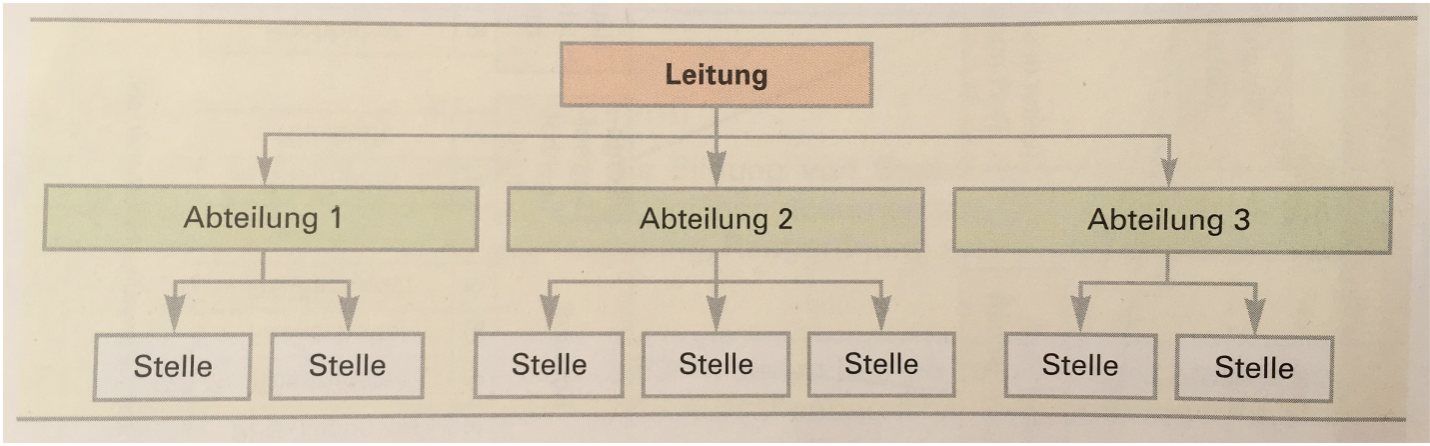
\includegraphics[height=6cm]{einlinien.png}
  \end{center}
  \caption{Einliniensystem}
  \label{fig:Einliniensystem}
\end{figure}
\textbf{Positives}:
\begin{itemize}
\item \"Ubersichtlich
\item Eindeutige und Abgegrenzte Dienstwege/Zust\"andigkeiten
\item Keine Kompetenz\"uberschneidungen
\item Starke Kontrollmöglichkeiten des Vorgesetzen nach unten
\end{itemize}
\textbf{Negatives}:
\begin{itemize}
\item Überlastung der Führungsebene mit Routineaufgaben (Informationsweitergabe)
\item Lange Dienstwege mit dem Risiko der Zeitverzögerung
\item Bei Großunternehmen besteht das Risiko einer Überorganisation/Bürokratisierung
\item Zwischeninstanzen können Informationen verfälschen oder unterdrücken
\item Wenig Spielraum für eigenverantwortliches Handeln
\end{itemize}
\textbf{Fazit}:
Da mit zunehmender Betriebsgröße auch die Anzahl der Hierarchieebenen steigt, führt dies zunehmend zu Unüberschaubarkeit und langen Informationswegen. \\
Damit erhalten die Nachteile ein immer stärkeres Gewicht. \\
Die wenig wertschöpfenden Routineaufgaben binden mehr und mehr die kostbaren Ressourcen der Führungsebenen und die Unzufriedenheit der mündigen, aber eingeengten Mitarbeiter steigt. \\
Das Einliniensystem eignet sich daher nur für kleinere Betriebe.

\subsubsection{Mehrliniensystem}
Kennzeichen:
\begin{itemize}
\item Ein Mitarbeiter kann von mehreren übergeordneten Vorgesetzten (Funktionsstellen) fachliche Anweisungen erhalten
\item Im Gegensatz leitet er Berichte und Meldungen auch an die jeweilige übergeordnete Stelle zurück
\end{itemize}
\begin{figure}[H]
\begin{center}
  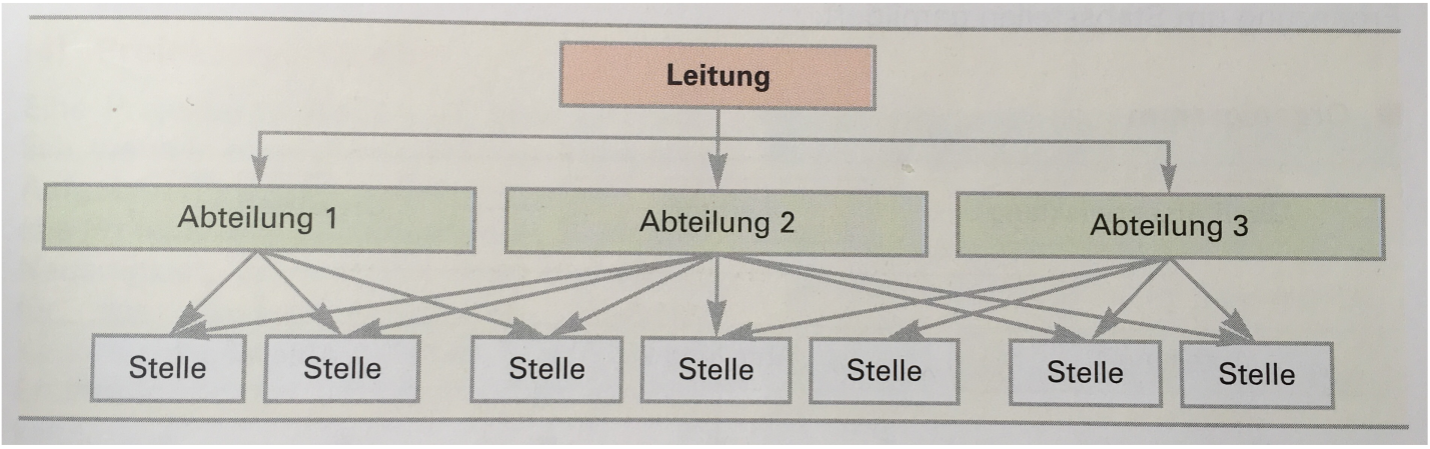
\includegraphics[height=6cm]{mehrlinien.png}
  \end{center}
  \caption{Mehrliniensystem}
  \label{fig:Mehrliniensystemm}
\end{figure}
\textbf{Positives}:
\begin{itemize}
\item Entlastung der Führungsebenen von Routinearbeiten 
\item Instanzenwege werden verkürzt
\item Die betrieblichen Hierarchien werden flacher
\item Das Unternehmen kann flexibler reagieren
\item Stelleninhaber können sich spezialisieren
\end{itemize}
\textbf{Negatives}:
\begin{itemize}
\item Instanzenaufbau wird unübersichtlicher
\item Erheblicher Abstimmungsaufwand
\item Reibungsverluste, Verunsicherung und Überlastung des Stelleinhabers bei konkurrierenden statt kooperierenden Vorgesetzten
\item Bei nicht klar abgegrenzten Kompetenzen besteht das Risiko von Konflikten
\end{itemize}
\textbf{Fazit}:
Mit zunehmender Betriebsgröße steigt die Komplexität der Gesamtaufgabe, sodass nur Spezialisten im Team diese Aufgaben bewältigen können. \\
Die Verkürzung der Instanzenwege durch ein fachliches Weisungsrecht in direktem Durchgriff entlastet von Routineaufgaben und erhöht damit die Effizienz des Gesamtsystems. \\
So hat z.B. der Ausbildungsleiter für alle Fragen der Berufsausbildung eine Weisungsbefugnis gegenüber allen Auszubildenden in den verschiedenen betrieblichen Aufgaben.

\subsubsection{Stabliniensystem}
Kennzeichen:
\begin{itemize}
\item Die Stabstellen sind gegenüber den ihnen zugeordneten Leitungsstellen weisungsgebunden
\item Stabstellen liegen außerhalb des Instanzenaufbaus
\item Sie haben keine Weisungsbefugnis gegenüber den nachgeordneten Stellen, wohl aber ein Informationsrecht, wenn sie Auskünfte anderer Stellen zur Bewältigung ihrer Aufgabe benötigen
\item Typische Aufgaben von Stabstellen: Beratung der Leitungsstelle, Begutachtung, Prüfung, Informationsbeschaffung und deren Auswertung, Entscheidungsvorbereitung, Erstellung von Richtlinien
\item Beispiele: EDV, Organisation, Qualitätsentwicklung, Unternehmensplanung
\end{itemize}
\begin{figure}[H]
  \begin{center}
  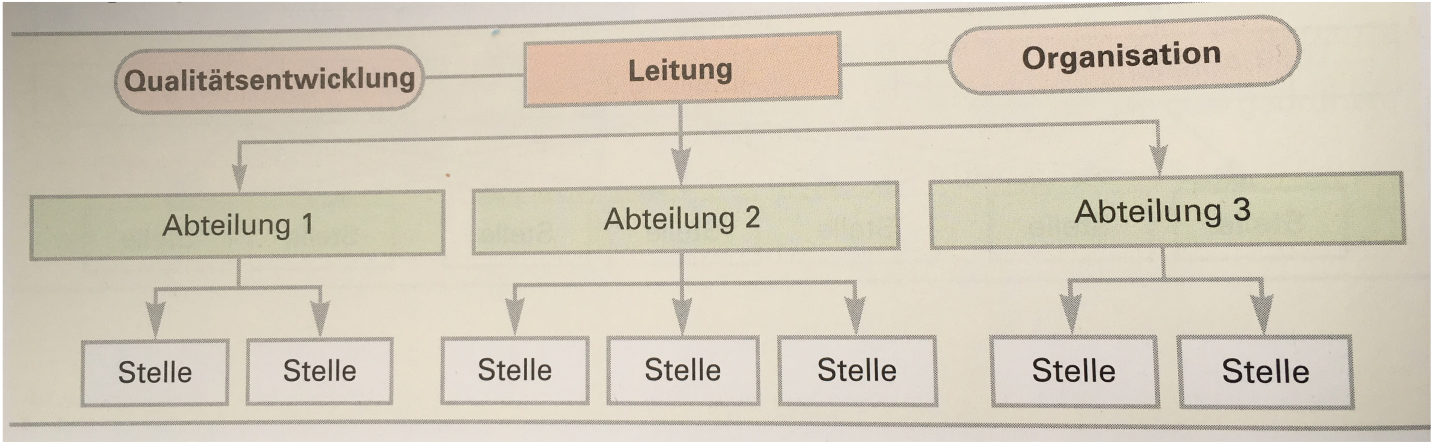
\includegraphics[width=12cm]{stablinien.png}
  \end{center}
  \caption{Stablinien}
  \label{fig:Stablinien}
\end{figure}
\textbf{Positives}:
\begin{itemize}
\item Vorteile des Einliniensystems
\item Die Entscheidungsbasis der Führungsebenen wird durch qualifizierte Stabstellen verbessert
\item Nachwuchskräfte sammeln Erfahrung durch ihre Mitarbeit in verschiedenen Stabstellen
\end{itemize}
\textbf{Negatives}:
\begin{itemize}
\item Grundprobleme des Einliniensystems werden nicht völlig beseitigt (z.B. lange Dienstwege)
\item Personalkosten steigen durch teure Spezialisten in den Stäben
\item Risiko, dass aufgrund der hohen fachlichen Kompetenz in den Stabstellen deren Einfluss auf die Geschäftsleitung sehr groß wird
\item Liniensysteme können gute Vorschläge der Stabsstellen weiterhin unterbinden 
\end{itemize}
\textbf{Fazit}:
Das Stabliniensystem bewahrt die Vorteile des Einliniensystems. \\ 
Es unterstützt die Geschäftsführung in der Qualität ihrer Entscheidungen wirkungsvoll durch die fachliche Kompetenz der Stäbe und vermeidet gleichzeitig die organisatorischen Risiken des Mehrliniensystems.

\subsection{Kritik an der Aufbauorganisation}
Die Aufbauorganisation führt zu Nachteilen, denn die Anstrengungen der einen Abteilung im Sinne des Gesamtunternehmens gewinnmaximierend zu handeln, kann den Anstrengungen der anderen Abteilungen zuwiderlaufen.
\begin{itemize}
\item Gefahr, dass sich Mitarbeiter an mengenmäßiger Leistung orientieren, nicht an Kunden, Arbeitsqualität oder Termintreue
\item Arbeitszerlegung fährt zu Tätigkeiten mit geringem Arbeitsinhalt, Monotonie und einseitiger Belastung. Selbstst\"andigkeit, Selbstverwirklichung k\"onnen weniger verwirklicht werden.
\item i.d.R verlaufen betriebliche Prozesse "quer" zu den Funktionen
\end{itemize}

\subsection{Qualitätsmanagement}
Beinhaltet alle Maßnahmen zur
\begin{itemize}
\item Planung
\item Steuerung
\item Optimierung
\end{itemize}
von Prozessen im Unternehmen. \\
Das Ziel ist es, eine bestimmte Qualität von Produkten /  Dienstleistungen zu erreichen. \\
Sie orientiert sich an Kundenwünschen, Meinungen und Feedback als auch messbaren  Merkmalen wie messbarer Qualit\"at.  \\
Die Produktqualität wird wie folgt gesichert:
\begin{itemize}
\item Interne/Externe Audits
\item \"Uberwachung von Prozessabl\"aufen
\item Erstellung von Analysen und Reports
\item Verantwortung für QM-Dokumentation
\item Planung, Umsetzung und Weiterentwicklung des QM-Systems
\item Mitarbeiter-Schulungen durchführen
\end{itemize}

\subsubsection{Total Quality Management (TQM)}
Es ist eine Erweiterung des traditionellen QM und schließt Mitarbeiter, Prozesse und Systeme mit ein. \\
Das Ziel ist es, eine Kultur der kontinuierlichen Verbesserung zu schaffen. 

\subsubsection{Kontinuierlicher Verbesserungsprozess (KVP)}
Zentraler Bestandteil des QM. \\
Es geht darum, kontinuierlich Verbesserungen im Unternehmen zu erzielen, indem man Prozesse optimiert, Probleme l\"ost und Innovationen vorantreibt. \\
Der Fokus liegt auf der st\"andigen Weiterentwicklung und Verbesserung von Produkten, Dienstleistungen und Prozessen

\subsection{Quantitativer Angebotsvergleich / Handelskalkulation}
\label{sec:Handelskalkulation}
Damit ein Unternehmen Gewinne erzielen kann, müssen die Verkaufspreise so kalkuliert sein, dass sowohl die \textbf{Kosten gedeckt} werden, als auch eine \textbf{Gewinnspanne} einberechnet wird. Dies nennt man, außerhalb von Industrieunternehmen, \textbf{Handelskalkulation}. \\
Durch die folgenden Verfahren, können auch Preise für mehrere Angebote eines Produktes berechnet werden. Die Berechnung und den Vergleich dieser Preise nennt man \textbf{Quantitativer Angebotsvergleich}, da hier nur auf Basis des Preises verglichen wird.
\begin{figure}[H]
\begin{center}
  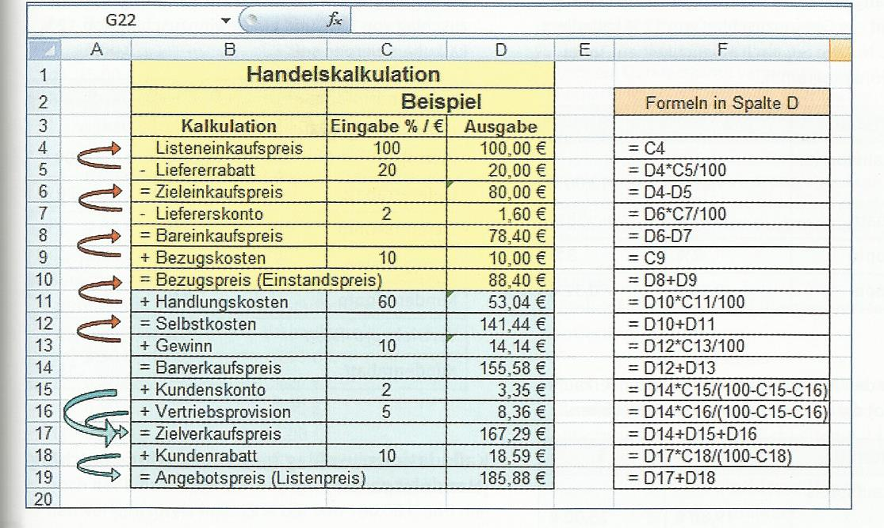
\includegraphics[height=6cm]{quantitativ.png}
  \end{center}
  \caption{Quantitativer Angebotsvergleich}
  \label{fig:Quantitativer Angebotsvergleich}
\end{figure}
Den gelben Teil nennt man auch \textbf{Bezugskalkulation}. \\
Der blaue Teil besteht aus der \textbf{Selbstkostenkalkulation} und \textbf{Absatzkalkulation}. \\ \\
Rechnet man vom Listeneinkaufspreis (oben) aus, so benutzt man die \textbf{Vorw\"artskalkulation}:
\begin{figure}[H]
\begin{center}
  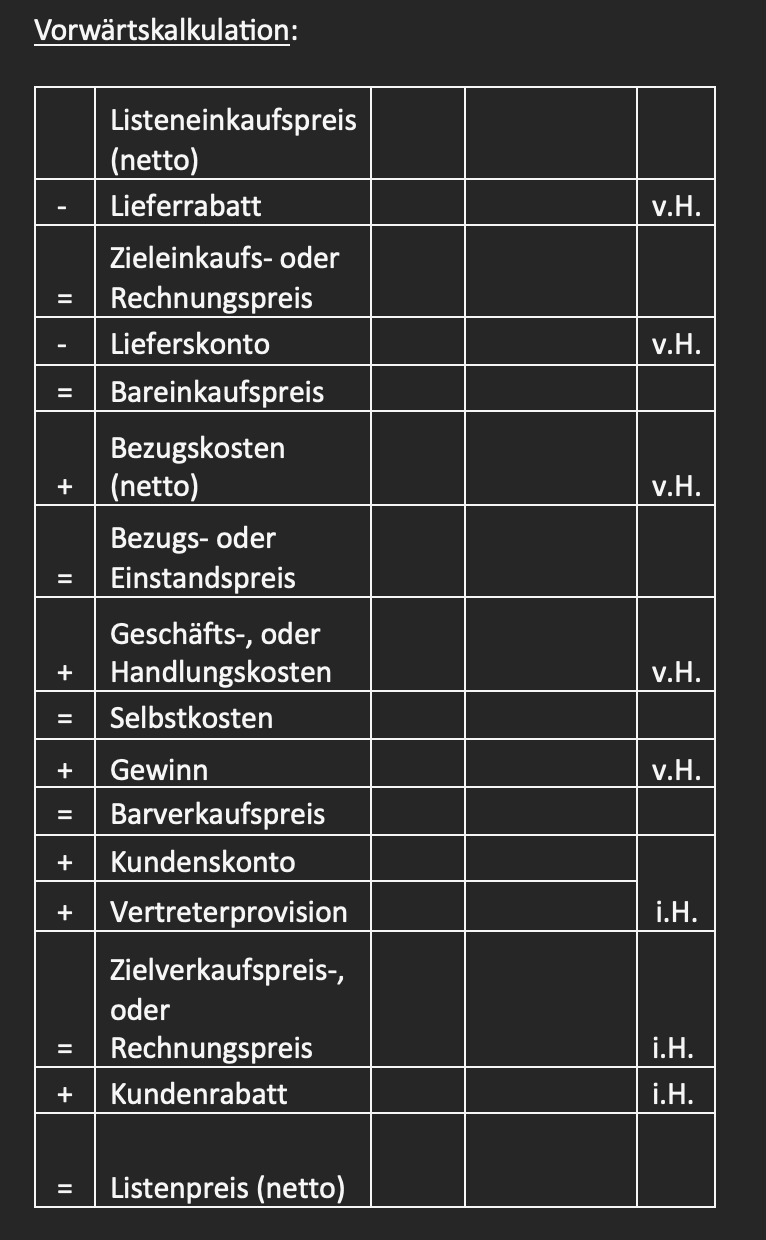
\includegraphics[height=12cm]{kalkV.png}
  \end{center}
  \caption{Vorwärtskalkulation}
  \label{fig:Vorwärtskalkulation}
\end{figure}
Hat man den Listenpreis (unten) gegeben, so benutzt man die \textbf{R\"uckw\"artskalkulation}
\begin{figure}[H]
\begin{center}
  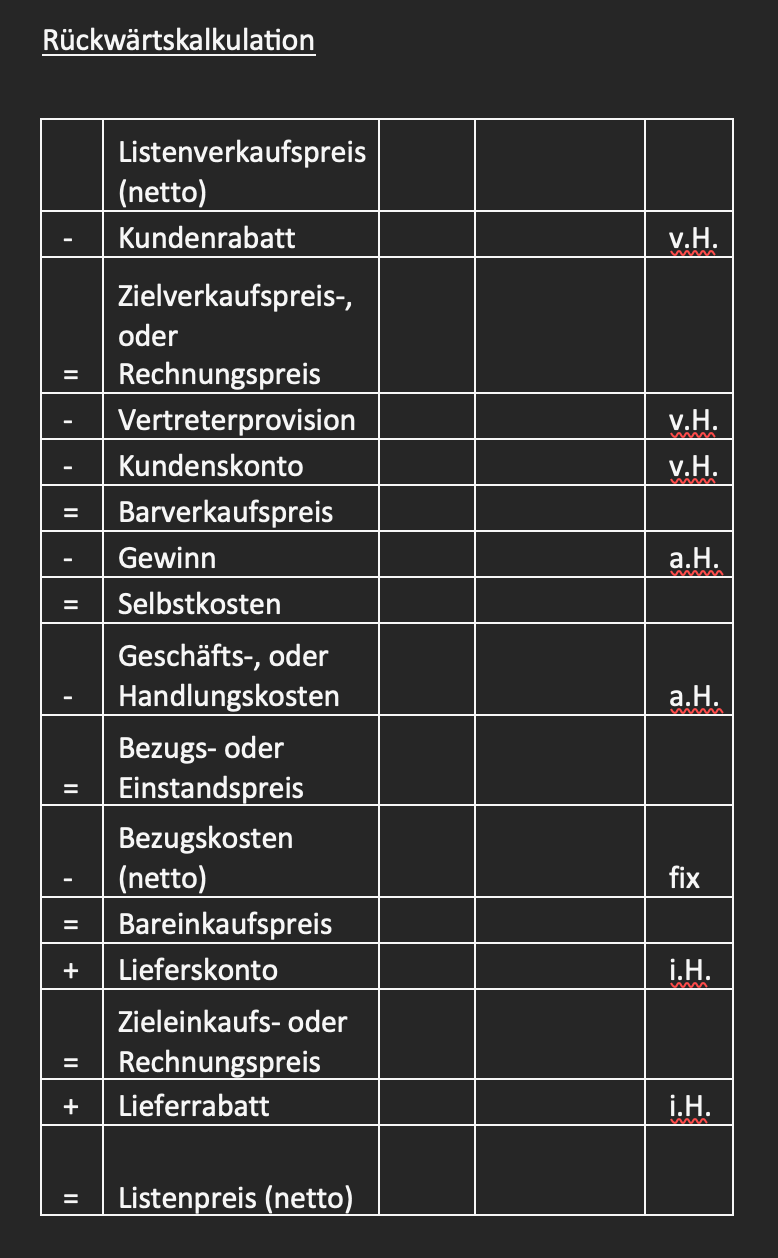
\includegraphics[height=12cmm]{kalkR.png}
  \end{center}
  \caption{Rückwärtskalkulation}
  \label{fig:Rückwärtskalkulation}
\end{figure}
Wenn man den Gewinn errechnen will, benutzt man die \textbf{Differenzkalkulation}:
\begin{figure}[H]
\begin{center}
  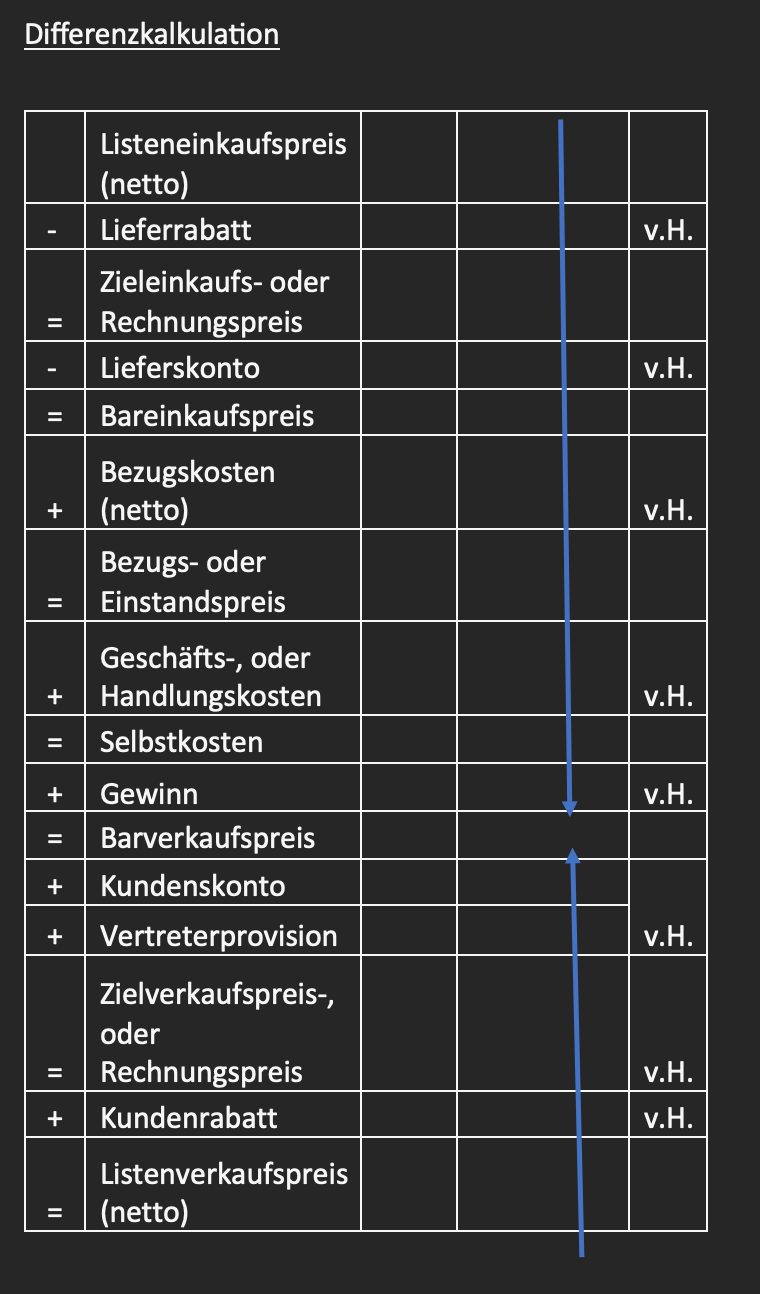
\includegraphics[height=12cm]{kalkD.png}
  \end{center}
  \caption{Differenzkalkulation}
  \label{fig:Differenzkalkulation}
\end{figure}
Um Zeit zu sparen kann man auch \textbf{verk\"urzte Kalkulationen} benutzen:
\begin{figure}[H]
  \begin{center}
  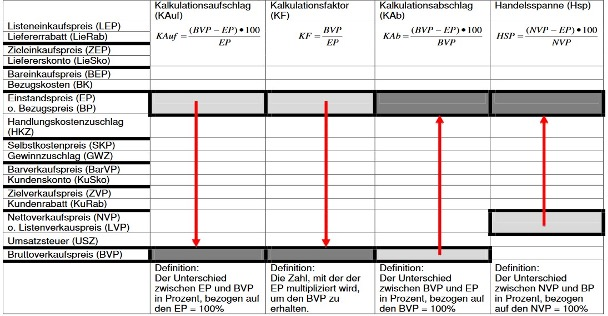
\includegraphics[width=12cm]{kalkS.jpg}
  \end{center}
  \caption{Verkürzte Kalkulation}
  \label{fig:Verkürzte Kalkulation}
\end{figure}

\break

\subsection{ABC-Analyse}

Die ABC-Analyse ist eine Methode zur Einteilung von Kunden, Produkten, Material und anderen Objekten in drei Klassen oder Kategorien: A, B oder C. \\
Die Objekte werden mit einer für die Analyse relevanten Kenngröße beschrieben und dann nach dieser Kenngröße sortiert. \\ \\
Schritt 1: $Menge * Preis$ \\
Schritt 2: Ordnen nach Preis in absteigender Reihenfolge \\
Schritt 3: Kumulativen Preis berechnen (vorherigen kumulativen Preis + Geradigen) \\
Schritt 4: Prozent ausrechnen (Prozent des kumulativen an der Stelle vom letzten \\ Kumulativen)
Schritt 5: Einteilen in Klassen
\begin{itemize}
\item[A] bis inklusive 80\%
\item[B] 81 bis inklusive 95\%
\item[C] 96 bis 100\%
\end{itemize}
\begin{figure}[H]
\begin{center}
  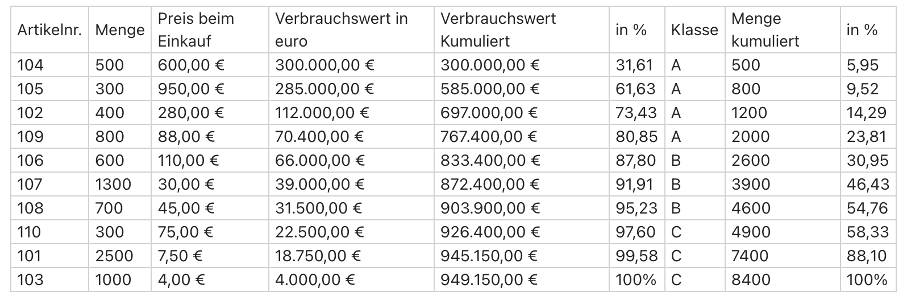
\includegraphics[width=12cm]{ABC.png}
  \end{center}
  \caption{ABC-Analyse}
\end{figure}

\subsection{Zahlungsverzug}
\begin{figure}[H]
\begin{center}
  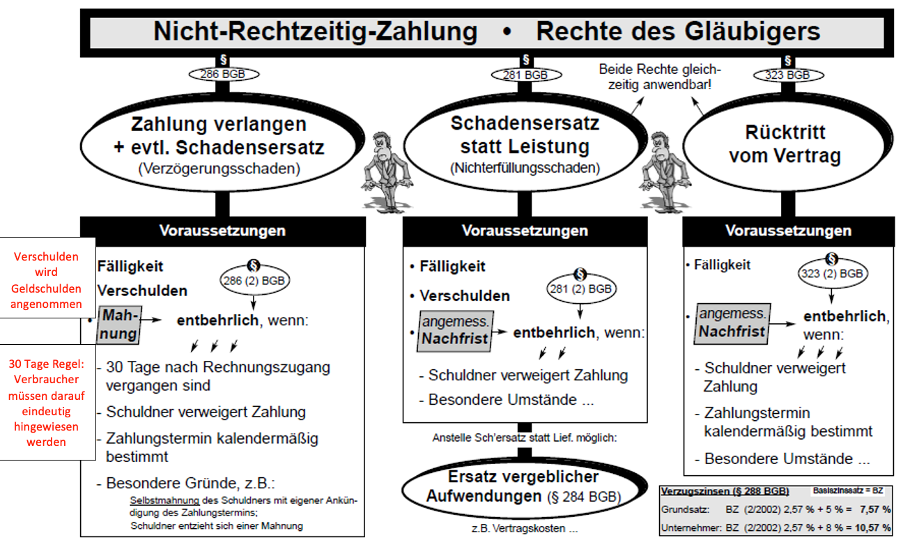
\includegraphics[width=12cm]{zahlungsverzug.png}
  \end{center}
  \caption{Zahlungsverzug}
  
\end{figure}
\subsubsection {Das außergerichtliche Mahnverfahren}
Gründe:
\begin{itemize}
\item[-] gute Geschäftsbeziehungen nicht gefährden
\item[-] Kunde könnte Zahlungstermin aus Versehen versäumt haben
\end{itemize}
\textbf {WICHTIG}: Rücksichtnahme ist hierbei schlecht, da eigene Zahlungsfähigkeit gefährdet wird

\subsubsection{Mahnstufen} 
Mahnstufe 1 (3 Tage nach Fälligkeit) - höfliche Zahlungserinnerung\\
Mahnstufe 2 (nach 7 Tagen) – 1. Mahnungsbrief\\
Mahnstufe 3 (nach 7 Tagen) – 2. Mahnung mit Rechnungsdurchschrift und Zahlungsträger\\
Mahnstufe 4 (nach 7 Tagen) – 3. Mahnung mit Androhung d. Forderungseinzugs\\
Mahnstufe 5 (nach 7 Tagen) – Forderungseinzug\\
Mahnstufe 6 (nach 7 Tagen) – letzte Mahnung mit Androhung gerichtlichem\\
Mahnverfahren oder Klage\\
(hierbei keine Beachtung der 30-Tage-Frist)\\\textbf{}

\subsection{Beschaffung}
\subsubsection {Geschäftsprozess Beschaffung und Lagerhaltung}
\begin{figure}[H]
\begin{center}
  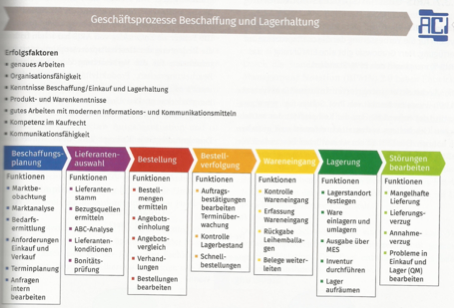
\includegraphics[width=12cm]{Beschaffung.png}
  \end{center}
  \caption{Zahlungsverzug}
\end{figure}

\subsubsection{Bedarfsermittlung}
\begin{itemize}
\item[1.] Auftragsbezogene Bedarfsermittlung: \\
Es wird der Bedarf anhand von konkreten Aufträgen und Stücklisten ermittelt, z.B. 100 Schränke, dafür werden 500m2 Holz benötigt.
\item[2.] Verbrauchsorientierte Bedarfsermittlung: \\
Es werden Vergangenheitswerte zugrunde gelegt, z.B. im Durchschnitt benötigen wir 300 Flaschen Holzkleber pro Jahr.
\end{itemize}

\subsubsection{Bestellverfahren}
\begin{itemize}
\item[•]Feste Bestellmenge: Es wird immer die gleiche Menge bestellt.  \\ Geeignet für Güter mit gleichmäßigem Verbrauch, die eher günstiger im Einkauf sind
\begin{itemize}
\item[+] wenig Aufwand
\item[+] kostengünstig
\item[-] nicht flexibel (passt sich nicht an Schwankung an)
\end{itemize}
\item[•]Variable Bestellmenge: Termine können fest sein. \\
Es wird immer genau die Menge bestellt, die gebraucht wird, geeignet für Güter mit Schwankungen in den Verkaufszahlen (z.B. saisonal bedingt) und höherpreisige Güter.
\begin{itemize}
\item[+]Immer die passende Menge auf Lager (nicht zu viel und nicht zu wenig)
\end{itemize}
\item[•]Optimale Bestellmenge: Summe aus Einstands-, Bestell- und Lagerkosten ist minimal
\end{itemize}

\subsubsection{Terminplanung}
\begin{itemize}
\item[•]Bestellpunktverfahren: Meldebestand und Mindestbestand werden festgelegt.\\
Menge kann fest oder variabel sein.
\item[•]Bestellrhythmusverfahren: sich wiederholende, festgelegte Liefertermin.\\
Man setzt hier meist die optimale Bestellmenge an.
\item[•]Einzelbeschaffung
\end{itemize}

Probleme beim Bestellrhythmusverfahren: \\
überhöhte Lagerbestände oder Fehlmenge.n\\
Der durchschnittliche Lagerbestand sinkt wenn häufiger bestellt wird bzw. der Sicherheitsbestand niedriger angesetzt wird.

\subsubsection{Ermittlung der Bestellmenge}
Bestellpunktverfahren:
Es wird die Veränderung der Lagerbestände über einen gewissen Zeitraum überprüft, um die Bestellmenge optimal zu planen

\begin{figure}[H]
\begin{center}
  \includegraphics[width=12cm]{Lagerbestandveränderungen.png}
  \end{center}
  \caption{Beispiel Lagerbestandver\"a"nderung}
  \label{fig:Lagerbestandveränderung}
\end{figure}

Das Schaubild zeigt die Lagerbestände eines Artikels. \\
Der Höchststand waren hier 200 Stück und einem regelmäßigen Verbrauch von 25 Stück pro Werktag. Der Bestand nimmt ständig ab und erreicht den Bestellpunkt/Meldebestand. Der Bestellpunkt ist der Zeitpunkt, zu dem bestellt wird während der Meldebestand die Menge ist, ab der  bestellt wird.\\
Die schwarze Kurve zeigt den Fall eines Meldebestandes von 50 Stück (Fall 1). Es werden dann 200 Stück bestellt, die nach zwei Tagen eintreffen, zum Punkt, an dem der Bestand auf 0 gesunken ist.
Im zweiten Fall (blaue Kurve) gibt es einen Sicherheitsbestand von 50 Stück und der Meldebestand beträgt jetzt 100 Stück. Wird der Höchstbestand beibehalten, muss jetzt häufiger in kleinerer Menge bestellt werden.


\begin{itemize}
 \item[1.]Durchschnittlicher Lagerbestand:
 \item[]Anfangsbestand = Mindestbestand + Bestellmenge
 \item[]Endbestand = Mindestbestand
 \item[]Durchschnittlicher Lagerbestand = (Anfangsbestand + Endbestand) / 2
\item[]Oder Monatsgenaue Berechnung: 
\item[]Durchschnittlicher Lagerbestand = (Anfangsbestand + 12 * Monatsendbestände) / 13

 \item[2.]	Höchstbestand = Mindestbestand + optimale Bestellmenge
 \item[3.]	Meldebestand = Mindestbestand + (Tagesverbrauch * Lieferzeit)                 \item[]Stellt sicher, dass rechtzeitig bestellt wird (Beschaffungszeit wird überbrückt, Sicherheitsbestand wird nicht unterschritten)
 \item[4.]	Mindestbestand oder Sicherheitsbestand: eiserne Reserve, wird von der Geschäftsleitung festgelegt, darf nur in Ausnahmefällen unterschritten werden; soll Bedarfsunsicherheit, Lieferzeitunsicherheit und Bestandsunsicherheit abdecken

\end{itemize}

\subsubsection{Bestellrhytmusverfahren}
Das Bestellrhythmusverfahren ist eine Strategie, die ein Unternehmen innerhalb der Lagerverwaltung verfolgt. Ziel des Bestellrhythmusverfahrens ist es, den optimalen Zeitpunkt und die optimale Menge für die Materialbeschaffung festzulegen. Die zentralen Kennzahlen im Bestellrhythmusverfahren sind die optimale Bestellmenge und die Fehlmengenkosten.

\begin{figure}[H]
\begin{center}
    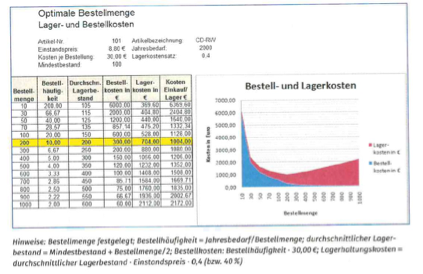
\includegraphics[width=12cm]{Bestellrhymusverfahren.png}
    \end{center}
    \caption{Beispiel Bestellrhytmusverfahren}
    \label{fig:my_label}
\end{figure}

\subsubsection{Eigenfertigung oder Fremdbezug (make or buy)?}
Man vergleicht bei freier Kapazität die Kosten bei Fremdbezug = Einstandspreis mit den variablen Herstellkosten bei Eigenfertigung. \\
Beispiel: Ein Industriebetrieb verkauft 7 verschiedene Produkte. Die Produkte 1 bis 5 werden im eigenen Unternehmen hergestellt.
Die Produkte 6 und 7 werden eingekauft und als Handelsware wieder verkauft.
Es ist Produktionskapazität frei.

\begin{figure}[H]
\begin{center}
  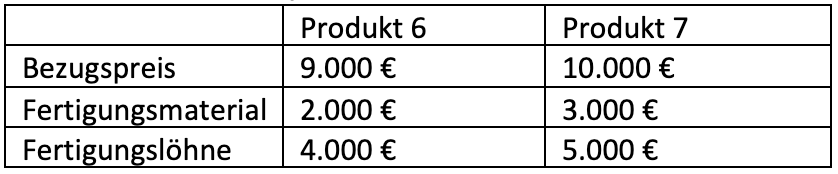
\includegraphics[width=12cm]{makeOrBuy.png}
  \end{center}
  \caption{Tabelle von Produkt 6 und 7}
  \label{fig:MakeOrBuy.png}
\end{figure}

\textbf{Materialgemeinkostenzuschlagssatz}: 25\%, davon 20\% variable Kosten./
Fix Kosten: unabhängig von der verkauften oder produzierten Menge z.B. Miete für Lagerräume/
Var. Kosten: ändern sich mit der verkauften oder produzierten Menge z.B. Stromkosten/
Fertigungsgemeinkostenzuschlagssatz: 120\%, davon 40\% variable Kosten.

\begin{figure}[H]
\begin{center}
  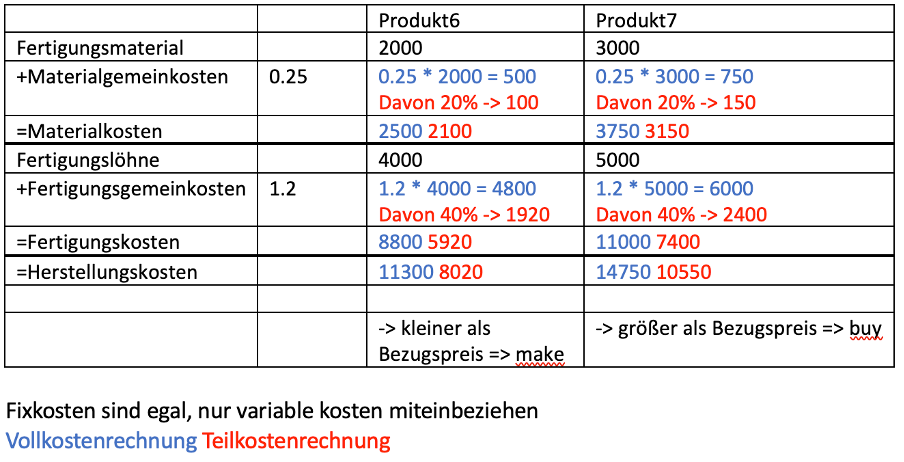
\includegraphics[width=12cm]{berechnungMakeOrBuy.png}
  \end{center}
  \caption{Tabelle zur Berechnung von Produkt 6 und 7}
  \label{fig:berechnungMakeOrBuy.png}
\end{figure}

\subsection{Kaufvertrag} 
Verkäufer verpflichtet sich die Ware mangelfrei an den Käufer zu geben. Dabei zahlt man nur für die Sache/Produkt. 
Sonderform: Verbrauchsgüterkauf (Unternehmen verkauft an Verbraucher)/
Fernabsatzvertrag (Unternehmen verkauft an Verbraucher fernmündlich z.B. Online Shopping)

\subsection{Werkvertrag} 
Auftragsnehmer(Werkunternehmer) verpflichtet sich ein konkretes Werk zu erstellen oder zu liefern  (z.B. Erstellung einer Software ). Bei offensichtlichen Mängel \textrightarrow\space Notierung ins Abnahmeprotokoll, bei schweren Mängel \textrightarrow\space Verweigerung der Abnahme möglich.

\begin{itemize}
    \item[-] Der Gegenstand wird speziell nach Kundenwunsch angefertigt
    \item[-]Der Verkäufer muss einen mangelfreien Gegenstand übergeben (Verjährungsfrist bei Mängeln: 3 Jahre)
    \begin{itemize}
        \item Ist dies nicht der Fall muss der Verkäufer nachbessern bis der Mangel beseitigt ist (Die Kosten hierfür trägt der Verkäufer)
    \end{itemize}

\end{itemize}

Abnahmeerklärung (s.u. Ende des Beschaffungsprozesses): Erklärung, dass eine Sache bestimmten Kriterien entspricht. Auftraggeber erklärt sein Einverständnis oder Ablehnung des vom Auftragsnehmer erstellten Werkes (ggf. Mängelanzeige)

Leistungen aus einem Werkvertrag: §640 BGB; Unternehmen hat Anspruch auf die Abnahme
Problem: wesentlicher Mangel, dann keine Abnahme; oft fiktive Abnahme; Folgen: Vergütung wird fällig, Gefahr der zufälligen Verschlechterung geht auf den Besteller über, nur bei Abnahme aufgenommene Mängel müssen beseitigt werden, Verjährung beginnt

Dienstvertrag: § 611 BGB, Dienst wird geschuldet, keine Abnahme, =Arbeitsvertrag, es gelten Kündigungsvorschriften


\subsection{Dienstleistungsvertrag} Eine Person oder ein Unternehmen erbringt eine Dienstleistung für eine andere Person oder ein anderes/gleiches Unternehmen (z.B. IT Support).\
Der Unterschied zwischen einem Werksvertrag und einem Dienstleistungsvertrag ist, dass ein Werksvertrag genaue und konkrete Anforderungen hat (z.B. App soll eine Filter Funktion erhalten). Der Dienstleistungsvertrag fokussiert sich eher auf die Dienstleistung/Service (IT Support: Laptop soll funktionieren)\\
Sonderform: Arbeitsvertrag
\begin{itemize}
    \item[-] Hier wird ein Dienst also Arbeitszeit gekauft
    \item[-]Es wird die Arbeitszeit bezahlt, die auch benötigt wird (d.h. wenn unerwartete Probleme auftreten/der Kunde nicht zufrieden ist oder man länger braucht, wird auch diese Zeit bezahlt)
\end{itemize}

Dienstleistungsverträge im IT-Bereich:\
\begin{itemize}
\item[-]IT-Sourcing: Dienstleistungen werden von extern beschafft
\item[-]IT-Outsourcing: unbefristete Auslagerung von IT-Aufgaben, IT-Abteilungen, IT-Bereichen mit Vertrag (auch nur selektiv möglich)
\item[-]Managed-Services: befristete Erledigung der Dienstleistungen durch externes IT-Systemhaus, mit Rahmenvertrag
\item[-]Desktop-Services: Hard- und Software werden bereitgestellt, erneuert und gewartet
\item[-]User-Helpdesk: Betreuung der Anwender im Unternehmen
\item[-]Cloud-Services: Infrastruktur, Plattform oder Software werden vom Dienstleister bereitgestellt
\item[-]Application Service Providing: über eine Datenleitung werden Anwendungen bereitgestellt, z.B. ERP-System
\item[-]On-Side-Management: Übernahme von Funktionen in den Räumen des Kunden, teilweise oder vollständig mit Betriebsmitteln des Kunden
\end{itemize}

\break

IT-Servicearten:
\begin{itemize}
\item[-]IT-Vertrieb, IT-Handel: Beschaffung von IT-Systemen und Komponenten, auch mit Aufbau und Anschluss an das vorhandene Netzwerk
\item[-]Break oder Fix-Support, Field Service, Vor-Ort-Service: Ausführung von IT-Dienstleistungen von Technikern vor Ort, Arbeitszeit+Anfahrtskosten+Teile werden in Rechnung gestellt
\item[-]Swap-Service: identisches Gerät wird als Ersatz zur Verfügung gestellt
\item[-]DIY-Service: Do-It-Yourself-Service, Kunde darf Servicearbeiten selbst durchführen (Gewährleistung bleibt)
\item[-]Live-Chat: über App oder ein Widget wird ein Chat-Kontakt zu einem Mitarbeiter hergestellt
\item[-]Garantieservice: unentgeltlich aufgrund von Gewährleistung oder Garantie
\item[-]IT-Einweisung, IT-Training, IT-Schulung
\item[-]Serviceverfügbarkeit
\item[-]Serviceportfolio, Servicekatalog
\end{itemize}


\begin{figure}[H]
\begin{center}
  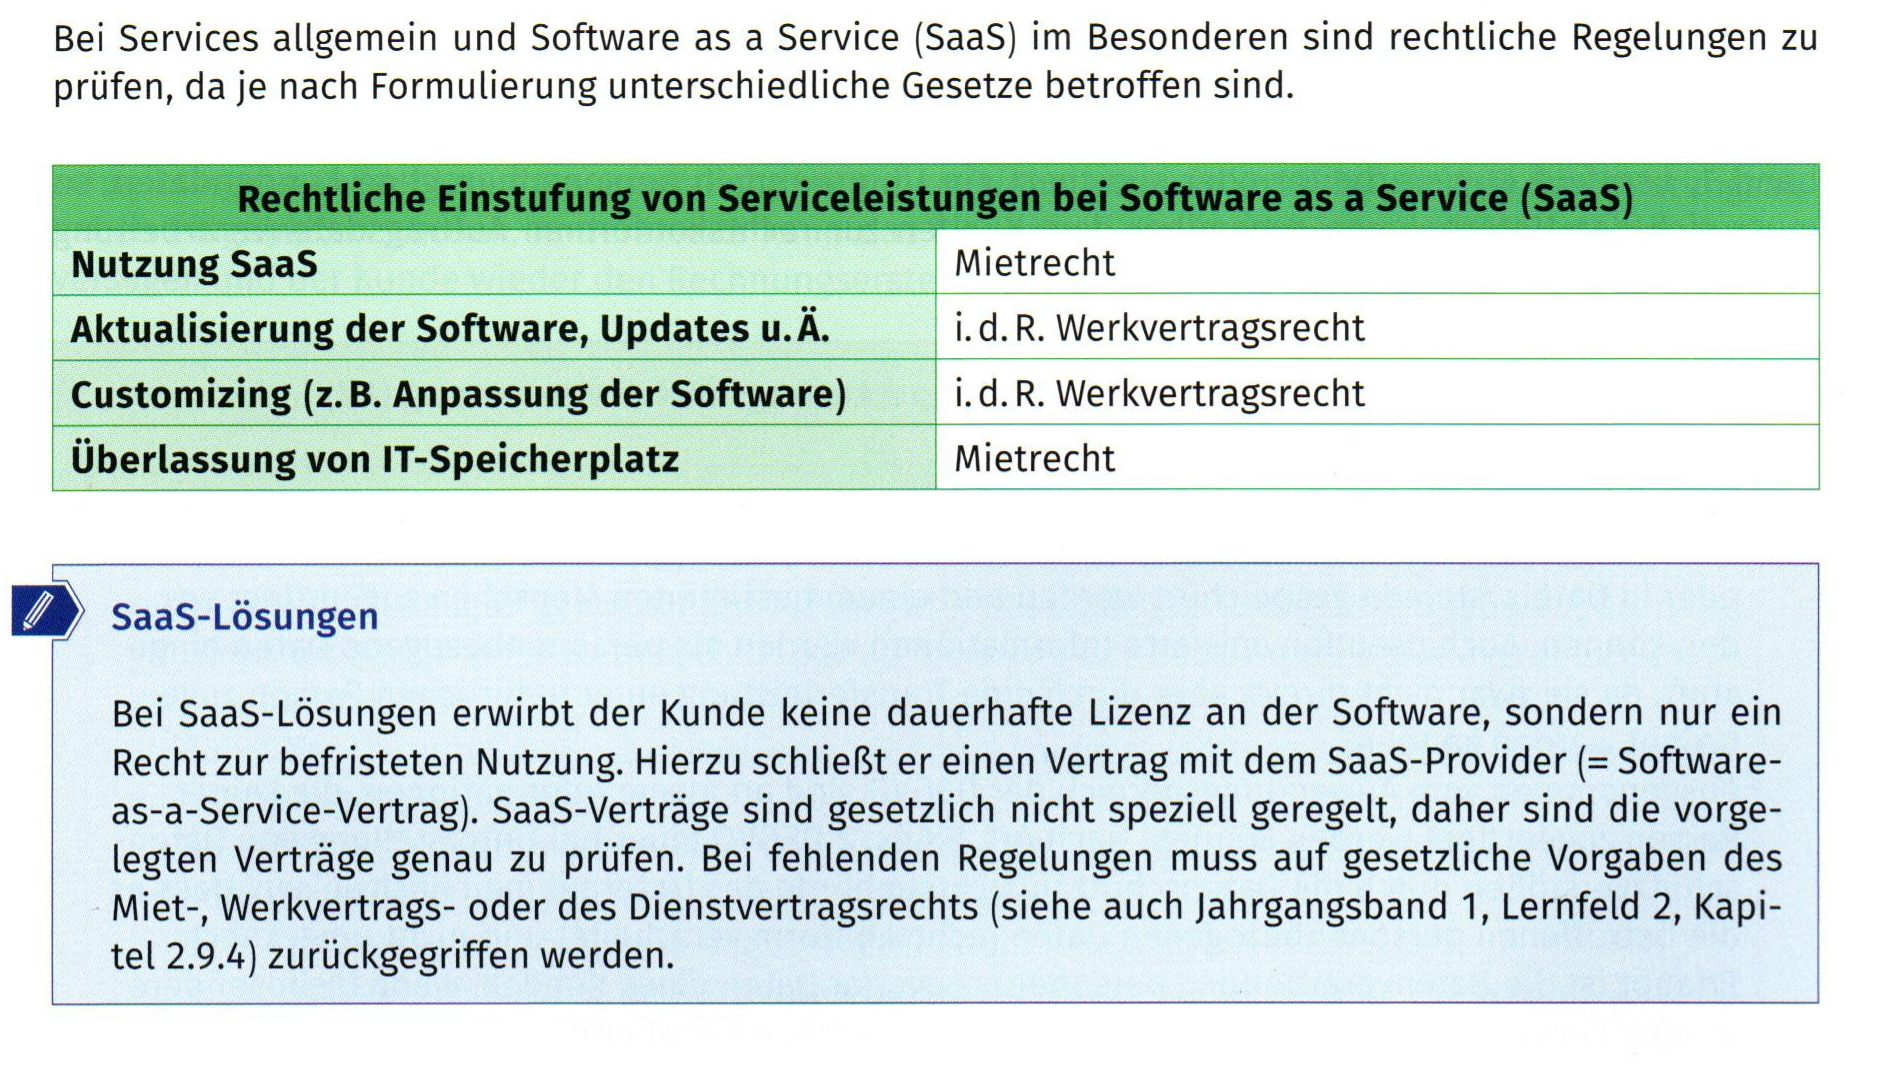
\includegraphics[width=12cm]{SaaS1.png}
  \end{center}
  \label{fig:saas1.png}
\end{figure}

\begin{figure}[H]
\begin{center}
  \includegraphics[width=12cm]{SaaS2.png}
  \end{center}
  \label{fig:saas2.png}
\end{figure}

\begin{figure}[H]
\begin{center}
  \includegraphics[width=12cm]{IT_Service.png}
  \end{center}

  \label{fig:IT_Service.png}
\end{figure}

\subsection{Ablauf eines Kaufvertrages}

\begin{figure}[H]
\begin{center}
  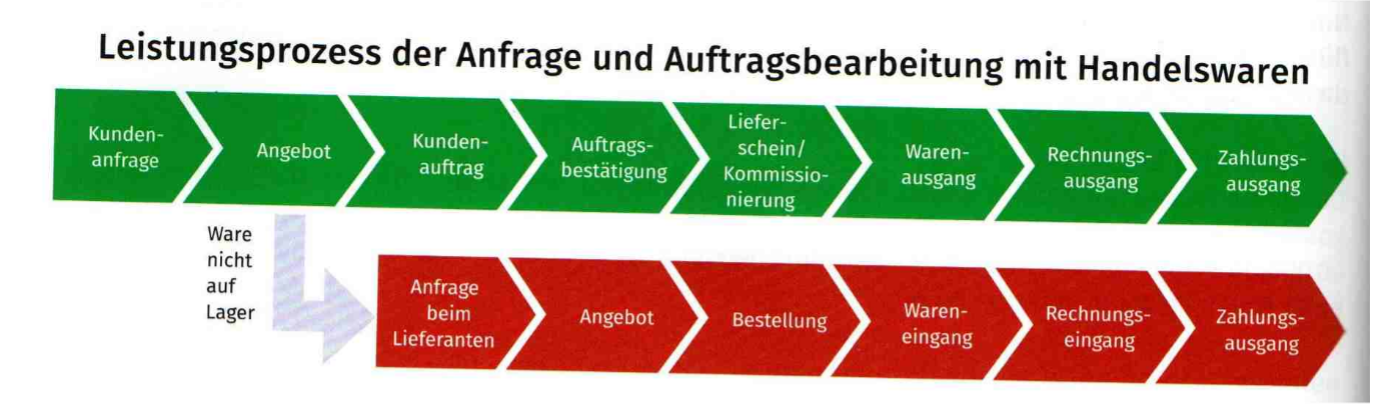
\includegraphics[width=12cm]{Kaufvertragablauf.png}
  \end{center}
\end{figure}

\begin{figure}[H]
\begin{center}
  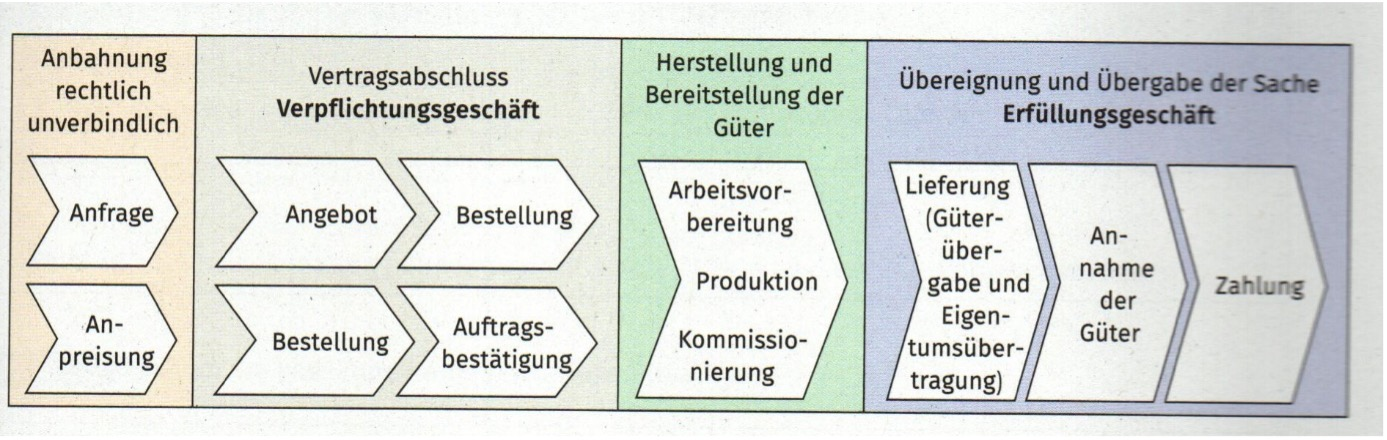
\includegraphics[width=12cm]{Kaufvertragablauf2.jpg}
  \end{center}
\end{figure}

\subsection{Angebotsvergleich}
\begin{figure}[H]
\begin{center}
  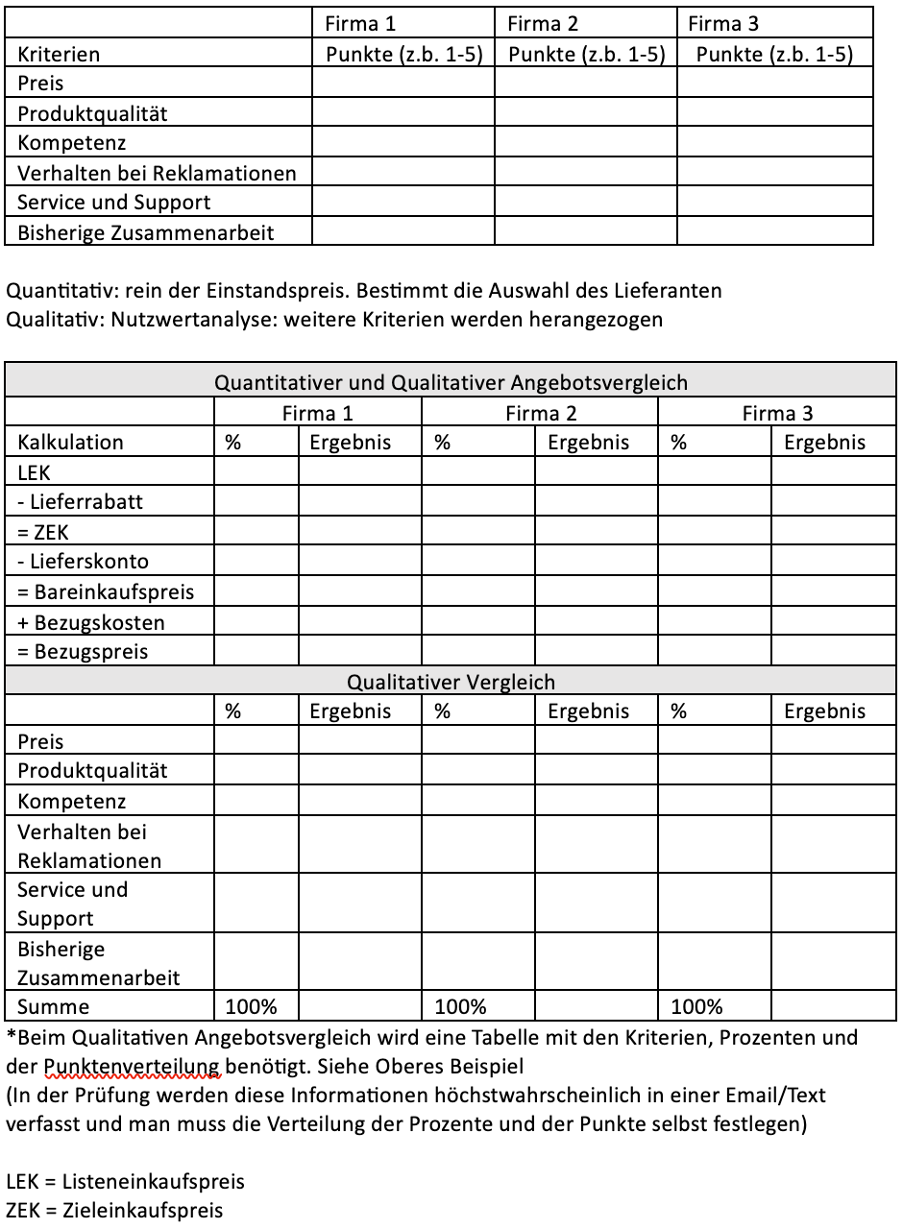
\includegraphics[width=12cm]{QuantitativUndQualitativerAngebotsvergleich.png}
  \end{center}
  \label{fig:QuantitativUndQualitativerAngebotsvergleich.png}
\end{figure}

\subsection{Ende des Beschaffungsprozesses}
(Wareneingang bzw. Abnahme der Leistung)

Ist die Warenlieferung im Eingangslager angekommen, wird sie geprüft, mit den Lieferpapieren verglichen und der Lagereingang im Computer erfasst. Durch elektronische Datenerfassung und Datenübertragung werden die Lieferdaten von den Lieferpapieren oder Verpackungen schnell aufgenommen, abgeglichen und dokumentiert. Bei einem Mangel wird eine Mängelanzeige im System oder auf einem Formular erstellt:

\begin{figure}[H]
\begin{center}
  \includegraphics[width=12cm]{Mängelanzeige.png}
  \end{center}
  \caption{Mängelanzeige}
  \label{fig:Mängelanzeige.png}
\end{figure}

Ist alles in Ordnung, wird die Lieferung im Vorratslager an den richtigen Platz gebracht, ansonsten häufig ein Platz in einem Zwischenlager gesucht. Ein weiterer wichtiger Arbeitsbereich im Lager ist das Ausgangs- oder Kommissionierungslager. Hier werden entsprechend dem Lieferschein oder Auftrag die Waren für den Kunden zusammengestellt, die verschiedenen Packstücke zu einer Ladeeinheit zusammengefasst und mit den Lieferpapieren für Kunden bestückt. Wenn die Lieferung vom Lieferanten schon für die Weiterlieferung an den Kunden verpackt wurde, wird sie gleich in das Ausgangslager gebracht. Bei der Warenannahme wird in zwei Schritten vorgegangen:

Äußerliche Sichtkontrolle in Anwesenheit des Überbringers und später eine genauere Kontrolle der Lieferung. Material- und Warenlieferungen müssen unverzüglich überprüft werden. 

\begin{figure}[H]
\begin{center}
  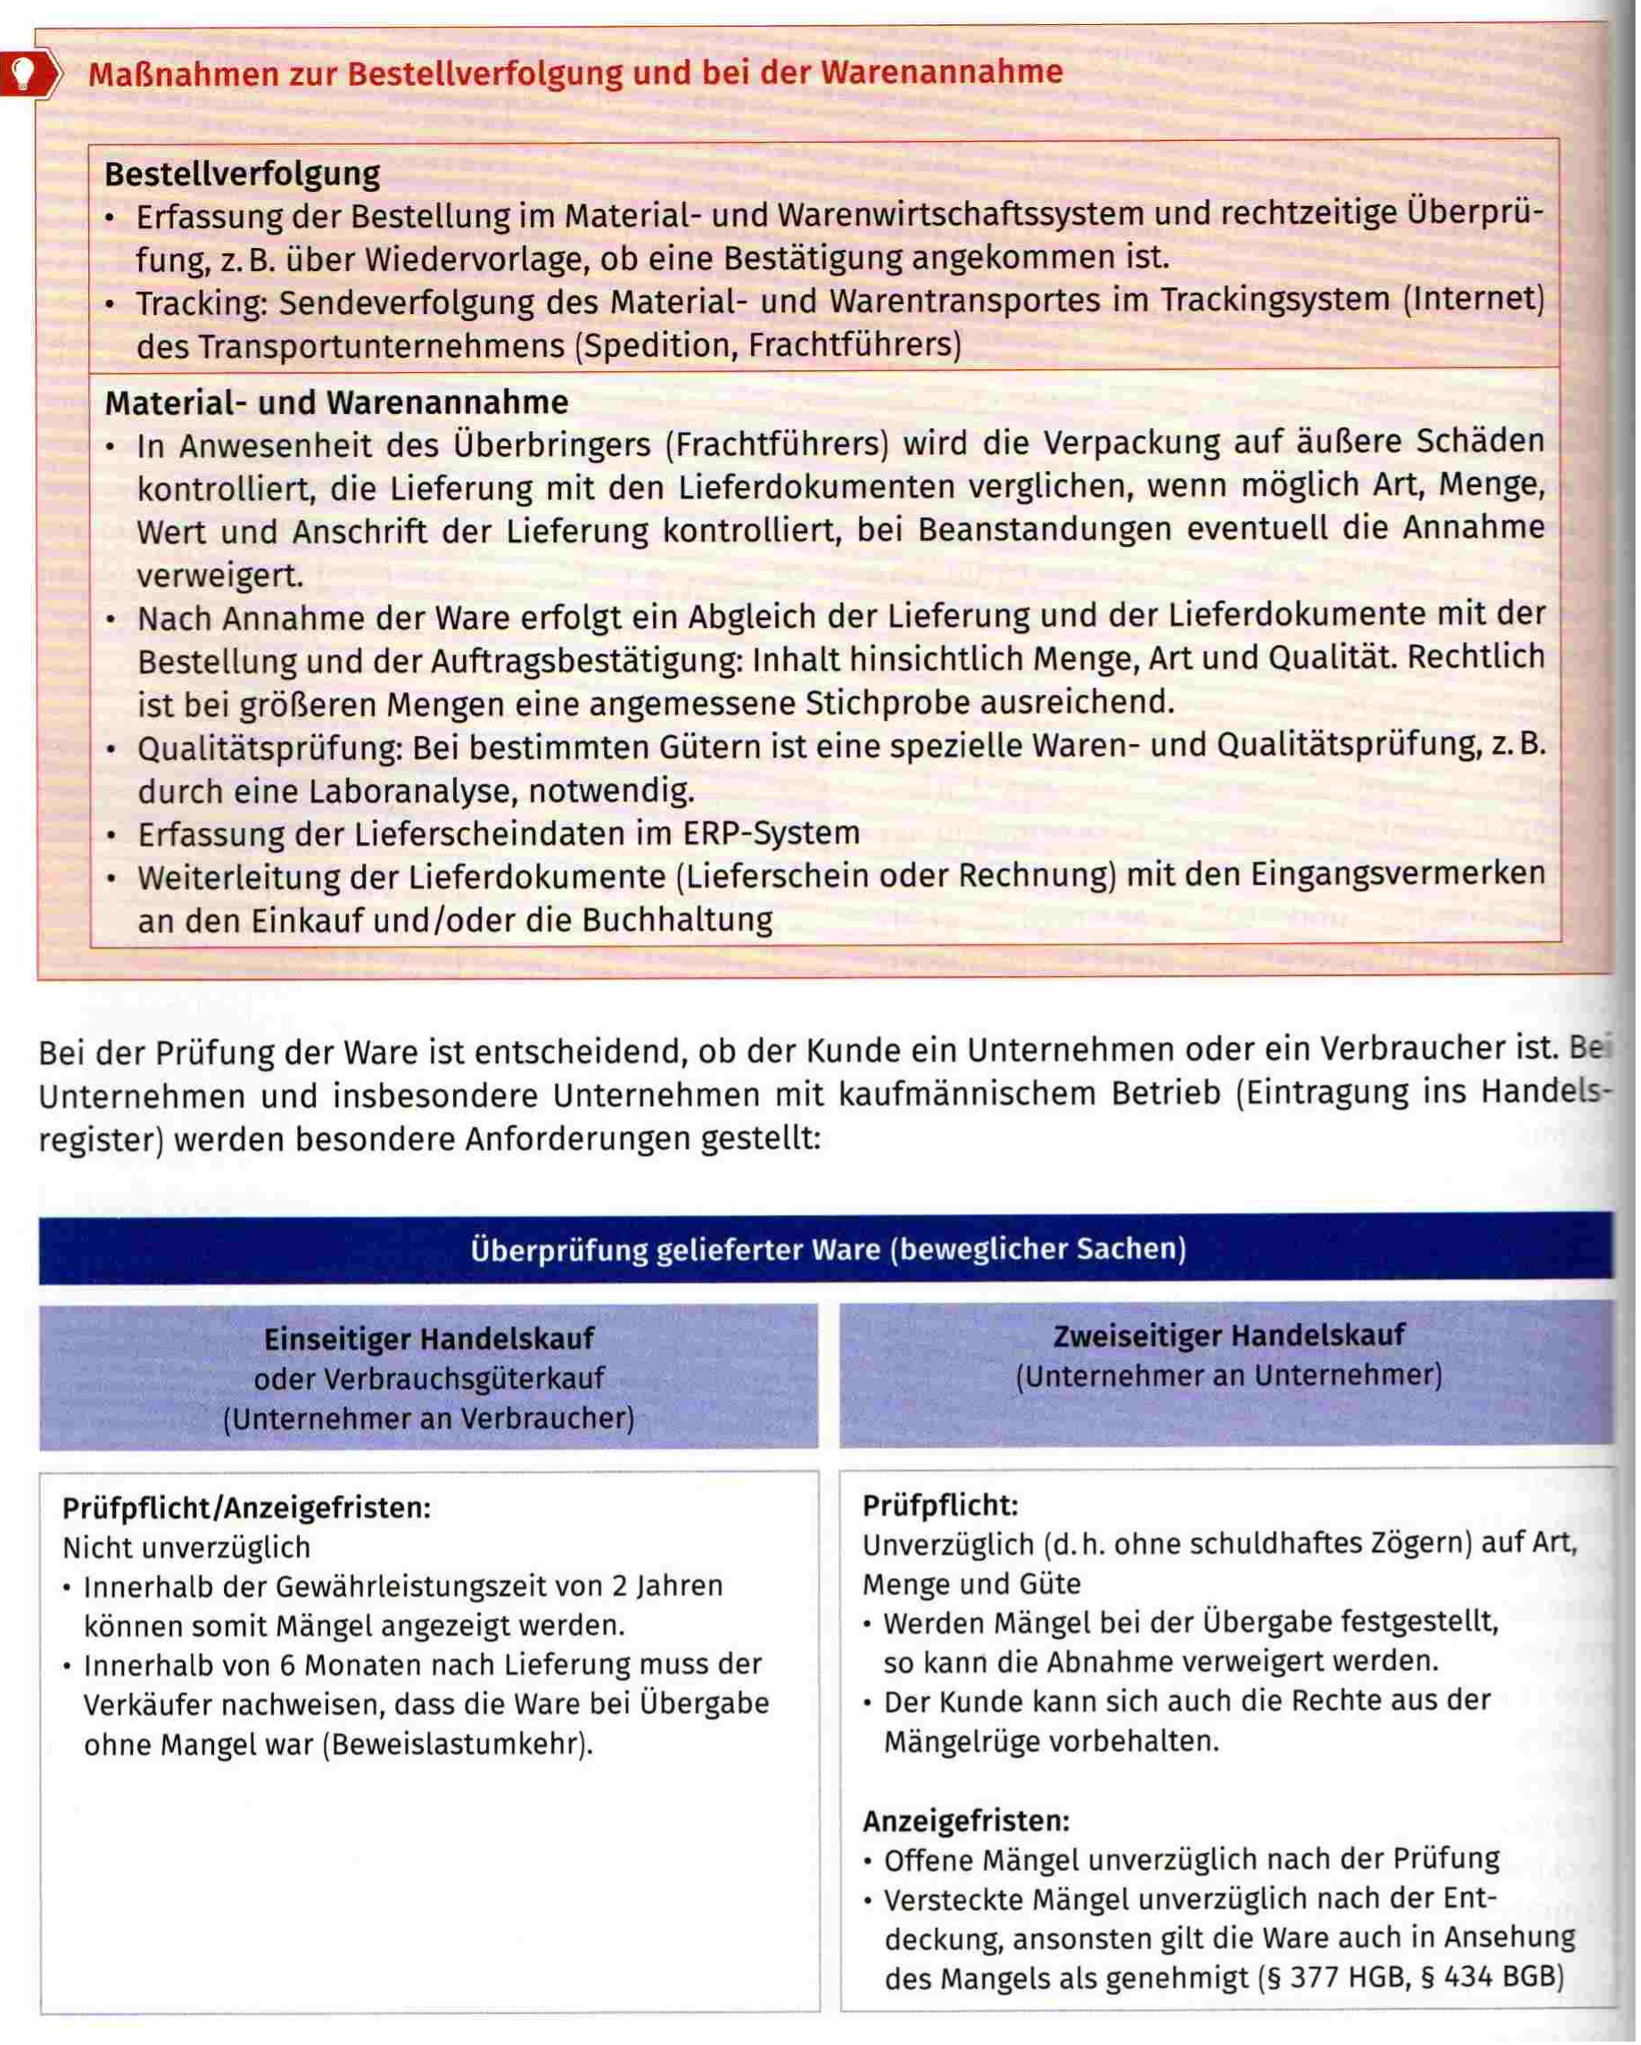
\includegraphics[width=12cm]{überprüfungWarenanahme.png}
  \end{center}
  \label{fig:überprüfungWarenanahme.png}
\end{figure} 

\subsubsection{Überprüfung der Rentabilität des Beschaffungsprozesses: TCO und ROI}

Unternehmen, Behörden und Organisationen müssen wirtschaftlich arbeiten. Daher sind alle Mitarbeiter aufgefordert, auf Wirtschaftlichkeit zu achten. Hierbei geht es nicht nur um den günstigsten Preis.

Folgende Aspekte sind zu beachten:
\begin{itemize}
	\item Preisvergleiche: Kostenbestandteil ist der Nettopreis, alle Rabatte, Skonto, sonstige Nachlässe müssen berücksichtigt werden.
	\item Anschaffungs- und Zusatzkosten: Maschinen, Systeme, Anlagen werden angeschafft. Hierbei sind die Bezugskosten, Installationskosten, Schulungskosten, Einarbeitungsaufwand u.a. in den Vergleich einzubeziehen.
	\item Folgekosten: Verbrauchskosten, Reparaturkosten, Wartungskosten u.a.
	\item Restwerte: Wertverlust der beschafften Güter = Abschreibungen
	\item Sonstige Kriterien: qualitativer Angebotsvergleich, z.B. Lieferantenqualität (s.o.)
\end{itemize}

\begin{figure}[H]
\begin{center}
  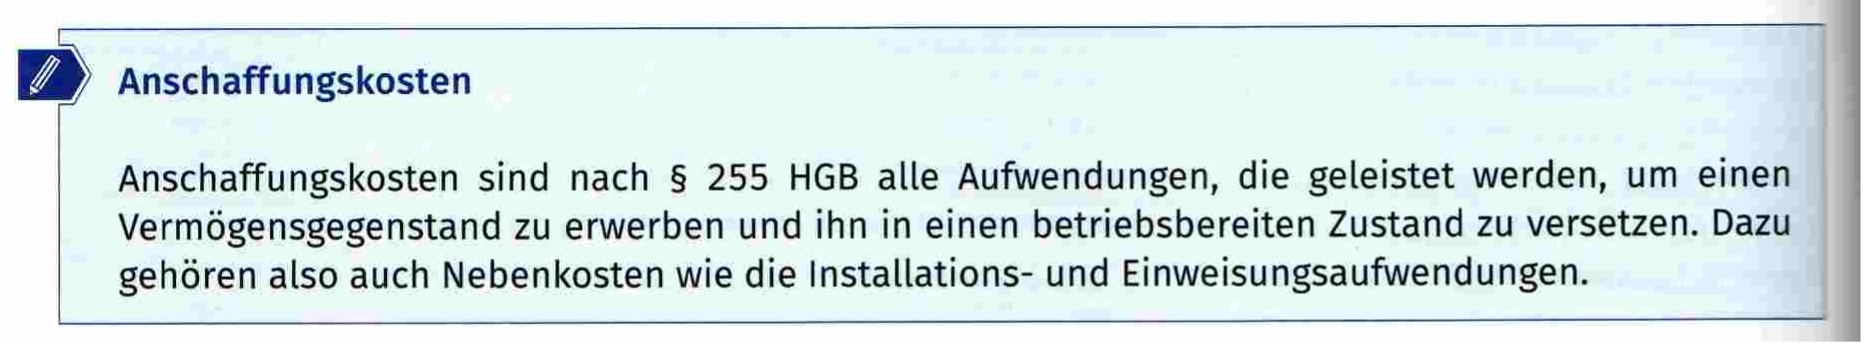
\includegraphics[width=12cm]{Anschaffungskosten.png}
  \end{center}
  \label{fig:Anschaffungskosten.png}
\end{figure} 

Mit der Berechnung des TCO geht man noch weiter und bezieht alle Kosten ein.
Da dies Zahlen der Zukunft sind, werden sie in einer Kalkulationsentscheidung geschätzt. Dabei muss man indirekte und direkte Kosten unterscheiden.

TCO = Total Cost of Ownership
Total Costs: Energie, Reparatur, Wartungskosten, Organisationskosten, Schulungskosten, Verwaltungsaufwand, Entschädigung für entgangene Geschäfte usw.

ROI = Return on Investment
Es geht hier um die Rendite einer Investition. Voraussetzung für die Berechnung des ROIs ist, dass sich Rückflüsse ergeben und ermitteln lassen (innerhalb der Nutzungsdauer).

\subsection{Besitz und Eigentum}
Besitz: Besitz ist die tatsächliche Herrschaft / Verfügbarkeit über eine Sache oder ein Recht. Der Besitzer kann mit der Sache nur im Rahmen von Vereinbarungen mit dem Eigentümer verfahren. (z.B. Mieter)

Eigentum: Eigentum ist die rechtliche Herrschaft / Verfügbarkeit über eine Sache oder ein Recht. Der Eigentümer kann mit der Sache beliebig verfahren, sofern dadurch nicht die Rechte Dritter verletzt werden. (z.B. Vermieter)

\subsubsection{Möglichkeiten der Eigentumsübertragung}
\textbf{Bei beweglichen Sachen:}

Einigung und Übergabe: 
Einigung zwischen Käufer und Verkäufer über die Übertragung des Eigentums im Rahmen des Erfüllungsgeschäftes und Übergabe, wenn der Gegenstand beim Verkäufer ist.\\
Beispiel: Der Verkäufer übergibt den gekauften Fotoapparat an den Käufer. Beide sind sich einig, dass das Eigentum übertragen wird.


Einigung: Käufer ist bereits Besitzer und wird durch die Einigung Eigentümer.
\begin{itemize}
    \item Beispiel: Nach Abschluss des Kaufvertrages wird der Käufer Eigentümer der vorher gemieteten Videoanlage (die sich in seinem Besitz befindet) nur aufgrund der Einigung über die Eigentumsübertragung. Eine Übergabe ist nicht mehr erforderlich.
\end{itemize}


Besitzkonstitut:
Einigung über die Eigentumsübertragung und Vereinbarung, dass der Verkäufer Besitzer bleibt.
\begin{itemize}
    \item Beispiel: Der Käufer erwirbt mehrere Wertpapiere von seiner Hausbank und belässt die Papiere weiterhin im Depot der Bank. Er wird Eigentümer der Wertpapiere durch die Vereinbarung, dass der Verkäufer weiterhin Besitzer bleibt und er das Eigentum erwirbt. (Käufer = mittelbarer Besitzer,- Verkäufer = unmittelbarer Besitzer)
\end{itemize}


Abtretung des Herausgabeanspruchs: 
Einigung über die Eigentumsübertragung und Abtretung des Anspruchs auf Herausgabe der Sache, wenn sich der Gegenstand bei einem Dritten befindet.
\begin{itemize}
    \item Beispiel: Der Verkäufer überträgt das Eigentum an einem Familienzelt durch die Vereinbarung, dass der Käufer gegenüber seinem Freund, dem er zur Zeit das Zelt geliehen hat, einen Herausgabeanspruch hat
\end{itemize}

\textbf{Bei unbeweglichen Sachen:}

Auflassung (Einigung) und Eintragung in das Grundbuch: 
Die Eintragung erfolgt, wenn die Auflassung nachgewiesen, die Eintragung beantragt und bewilligt wurde und die Bestätigung über die Zahlung der Grunderwerbssteuer vorliegt.

\textbf{Bei Rechten:}
Einigung über die Übertragung des Eigentums und Abtretung (=Zession)
Beispiel: Der Händler tritt seine Forderung an einen Kunden an seinen Lieferanten ab.

\textbf{Sonstiges:}

\textbf{Ersitzung:} 
Ist eine bewegliche Sache zehn Jahre im Eigenbesitz, so erfolgt die Eigentumsübertragung.

\textbf{Fund:}
Der Finder erwirbt unter bestimmten Umständen mit dem Ablauf von sechs Monaten nach Anzeige des Fundes das Eigentum.

\textbf{Verarbeitung, Vermischung, Verbindung:}
Es ist möglich, das Alleineigentum an der Sache zu erwerben.

\textbf{Gutgläubiger Erwerb:}
Gutgläubiger Erwerb liegt vor, wenn der Veräußerer für den Eigentümer gehalten werden durfte. Der gutgläubige Eigentumserwerb ist jedoch nicht möglich bei gestohlenen, verloren gegangenen oder
sonst abhanden gekommenen Sachen (Ausnahme: Geld, Inhaberpapiere).

\subsection{AGB}
\begin{figure}[H]
\begin{center}
  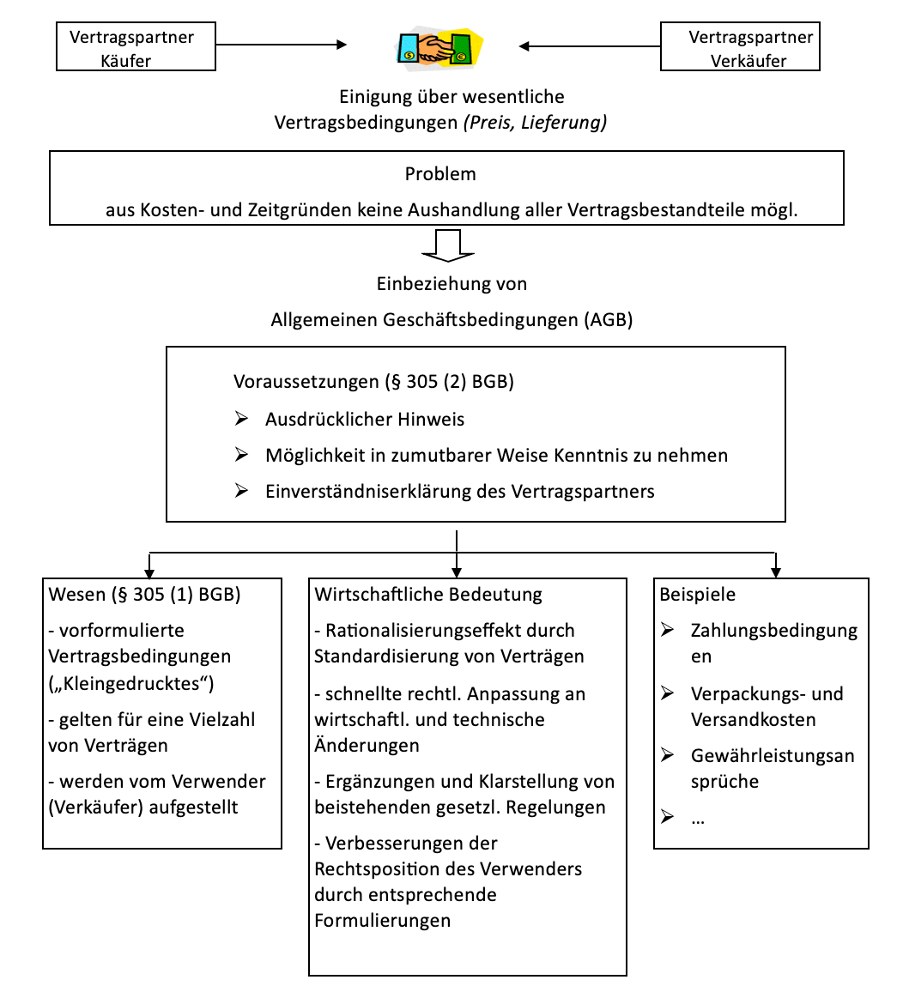
\includegraphics[width=12cm]{AGB.png}
  \end{center}
  \label{fig:AGB.png}
\end{figure} 

Unzulässige Bestimmungen in Allgemeinen Geschäftsbedingungen (AGB)
\begin{itemize}
    \item[-] Unangemessene Benachteiligung des Käufers
    \item[-]  Überraschende (ungewöhnliche) Klauseln
    \item[-]  Preiserhöhungen innerhalb von 4 Monaten nach Vertragsabschluss
    \item[-] Eine Bestimmung über unbestimmte Liefertermine ist unwirksam 
    \item[-]  Aufhebung oder Verkürzung der Gewährleistung für mangelfreie Ware
    \item[-]  Einschränkung von Gewährleistungsansprüchen 
    \item[-] Verpflichtung des Käufers zu einer Vertragsstrafe
    \item[-]  Rücktritts- und Änderungsrecht des Verkäufers
    \item[-]   Ausschluss des Rechts des Käufers auf Rücktritt vom Vertrag bei mangelhafter Lieferung  
\end{itemize}

\subsection{Fernabsatzverträge}
\begin{figure}[H]
\begin{center}
  \includegraphics[width=12cm]{Fernabsatzverträge.png}
  \end{center}
  \label{fig:Fernabsatzverträge.png}
\end{figure} 

\section{Hägele ITS}

\subsection{Strukturierte Verkabelung}

Eine strukturierte Verkabelung ist ein einheitlicher Aufbauplan für eine Netzwerkinfrastruktur, auf der unterschiedliche Dienste (Sprache oder Daten) übertragen werden.

Es basiert auf einer allgemein gültigen Verkabelungsstruktur, die auch die Anforderungen mehrerer Jahrzehnte berücksichtigt, Reserven enthält, flexibel erweiterbar ist und unabhängig von der Anwendung genutzt werden kann.

Durch diesen Plan sollen Fehlinstallationen vermieden und die Installation neuer Netzwerkkomponenten erleichtert werden.

\break

Es wird in 3 Bereiche unterschieden:
\begin{itemize}
    \item Geländeverkabelung (Prim\"ar)
        \begin{itemize}
            \item große Distanz
            \item große \"Ubertragungsraten
            \item meist Glasfaser
        \end{itemize}
    \item Gebäudeverkabelung (Sekund\"ar)
        \begin{itemize}
            \item kurze bis mittlere Distanz
            \item Kabel vom Geb\"audeverteiler zu Etagenverteilern
            \item Glasfaser oder Kupfer
            \item max 500m
        \end{itemize}
    \item Etagenverkabelung (Terti\"ar)
        \begin{itemize}
            \item kurze Distanz
            \item Twisted-Pair-Kabel
            \item max 90m
            \item M\"undung in Anschlussdosen
        \end{itemize}
\end{itemize}
\begin{figure}[H]
\begin{center}
  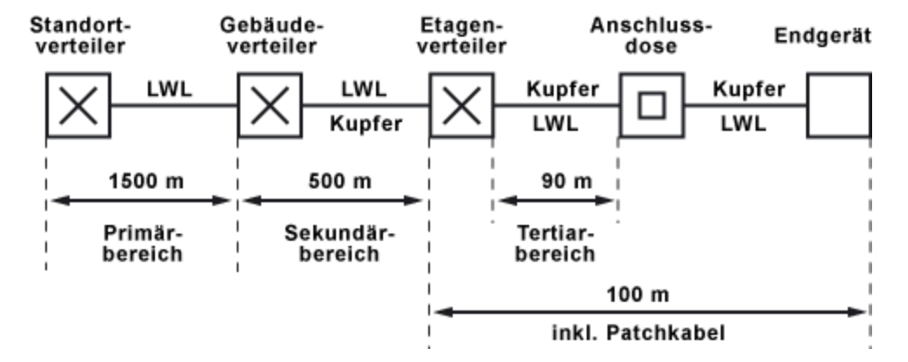
\includegraphics[height=6cm]{struk.png}
  \end{center}
  \caption{Strukturierte Verkabelung}
  \label{fig:Strukturierte Verkabelung}
\end{figure}
\break

\subsection{IPv4}

Eine IPv4-Adresse folgt dem Schema:

\(<0-255>.<0-255>.<0-255>.<0-255>\)

Beispiel: 192.168.0.1

Es stehen 32 Bit zur Verfügung \textrightarrow\space \(2^{32}\) \textrightarrow\space ca. 4 Mrd. IPv4 Adressen

\textbf{Spezielle IPv4 Netze:}
\begin{itemize}
    \item 127.x.x.x /8 \textrightarrow\space Loopback/Localhost (gilt für gesamtes 127er Netz)
    \item private IPv4 Netze:
        \begin{itemize}
            \item 10.0.0.0 /8
            \item 172.16.0.0 /12
            \item 192.168.0.0 /16
        \end{itemize}
\end{itemize}

\subsubsection{IPv4 Subnetting}

Es wird zwischen zwei Arten des Subnettings unterschieden:
\begin{itemize}
    \item \textbf{Symmetrisch}: Es entstehen n gleich große Subnetze
    \item \textbf{Asymmetrisch}: Es entstehen unterschiedlich große Subnetze
\end{itemize}

\textbf{Symmetrisches Subnetting}

Vorgehensweise mit Beispiel:

Ausgangsnetz: 10.0.0.0 /8\\
Ziel: Netz in drei Subnetze aufteilen

\textbf{1. Schritt:} Anzahl der zusätzlichen Netzbits bestimmen:\\
Da das Netz in drei Subnetze zerlegt werden soll, benötigen wir zwei zusätzliche Netzbits.\\
Begründung: Die nächst höhere Zweierpotenz ist 4 \textrightarrow\space \(2^\textbf{2} = 4\) \textrightarrow\space Zwei zusätzliche Netzbits

\textbf{2. Schritt:} Subnetzmaske / Slash-Darstellung anpassen\\
Aus 10.0.0.0 /8 wird nun 10.0.0.0 /10

\textbf{3. Schritt:} Netze bilden\\
Für die NetzID der Netze werden alle verfügbaren Hostbits auf 0 gesetzt. Um die jeweiligen Subnetze zu bilden, müssen nur die hinzugefügten Netzbits hochgezählt werden (00 \textrightarrow\space 01 \textrightarrow\space 10). Das vierte so entstehende Subnetz kann für diese Aufgabe ignoriert werden, da nur nach drei Netzen gefragt ist.

Erstes Subnetz: \textbf{10.0.0.0 /10}\\
Zweites Subnetz: \textbf{10.64.0.0 /10}\\
Drittes Subnetz: \textbf{10.128.0.0 /10}

Genauere Darstellung \href{https://jodies.de/ipcalc?host=10.0.0.0&mask1=8&mask2=10}{hier}.

\break

\textbf{Asymmetrisches Subnetting}

Asymmetrisches Subnetting wird genutzt, um Subnetze für eine bestimmte Anzahl an Clients zu erstellen.

Vorgehensweise mit Beispiel:

Ausgangsnetz: 10.0.0.0 /8\\
Ziel: 2 * 500 Hosts \textbf{+} 3 * 16 Hosts 

\textbf{Immer mit dem größten Netz anfangen!} 

\textbf{1. Schritt:} Anzahl der Netzbits bestimmen:\\
Für Netze mit 500 Hosts: 9 Hostbits (\(2^\textbf{9} = 512\)) \textrightarrow\space \(32-9 = 23\) Netzbits.

Für Netze mit 16 Hosts: 5 Hostbits (\(2^\textbf{5} = 32\) \textbf{(Es werden 32 IPs benötigt, da 16 IPs nicht für 16 Hosts reichen - Broadcast und Netz-ID können nicht vergeben werden!)})\textrightarrow\space \(32-5 = 27\) Netzbits.

\textbf{Schritt 2:} Subnetze bilden:\\
Für die Bildung des ersten Subnetzes, muss nur die Subnetzmaske/Slash-Notation angepasst werden:\\
1. Subnetz: 10.0.0.0 /23; Broadcast: 10.0.1.255

Um das zweite Subnetz zu bilden, wird die Broadcast IP des vorherigen Netzes um eins erhöht. Dies ergibt die Netz-ID des zweiten Netzes:\\
2. Subnetz: 10.0.2.0 /23; Broadcast: 10.0.3.255

Das gleiche Prinzip wir für das zweite Netz kann nun fortgeführt werden.
3. Subnetz: 10.0.4.0 /23; Broadcast: 10.0.5.255

\textit{Wenn nach einer hohen Anzahl von Netzen gefragt ist, kann nach einem Muster in den Netz-IDs gesucht werden, um den Prozess zu beschleunigen. In diesem Beispiel erhöht sich der 3. Block der IP immer um 2.}

Für das vierte Subnetz (das erste mit der neuen Hostanzahl), kann der gleiche Prozess für die Netz-ID angewendet werden wie zuvor (Broadcast des letzten Netzes + 1 = Netz-ID des neuen Netzes). Allerdings muss hier darauf geachtet werden, dass die Subnetzmaske/Slash-Notation angepasst wird!\\
4. Subnetz: 10.0.6.0 /27; Broadcast: 10.0.6.31

Für das fünfte Subnetz wird wieder die Broadcast IP des vorherigen Netzes um eins erhöht\\
5. Subnetz: 10.0.6.32 /27


\break
\subsection{IPv6}

Eine IPv6 Adresse folgt dem Schema:

\textless0-ffff\textgreater:\textless0-ffff\textgreater:\textless0-ffff\textgreater:\textless0-ffff\textgreater:\textless0-ffff\textgreater:\textless0-ffff\textgreater:\textless0-ffff\textgreater:\textless0-ffff\textgreater

Beispiel: fe80:0000:0000:0000:7d45:0db9:c2c2:ab7b

Es stehen 128 Bit zur Verfügung \textrightarrow\space \(2^{128}\) \textrightarrow\space ca. \(3.4 * 10^{38}\) IPv6 Adressen (340 Sextillionen).

Die IPv6 Adresse wird in 8 Blöcke mit jeweils 16 Bit unterteilt, die durch ein ':' getrennt werden.\\
Innerhalb eines Blocks dürfen \textbf{führende} Nullen weggelassen werden.\\
Eine Folge von 0er-Blöcken darf \textbf{einmalig} durch '::' ersetzt werden.

Die Beispiel Adresse lässt sich so wie folgt kürzen:\\
fe80::7d45:db9:c2c2:ab7b

Die ersten vier Blöcke bilden den Prefix (Netzbits) und die letzten 4 den Identifier (Hostbits) der IPv6 Adresse.

\subsubsection{Der Identifier}
Der Identifier wird nach EUI64 aus der MAC Adresse des Gerätes gebildet und kennzeichnet den Host. Dabei wird in die Mitte der MAC Adresse 'fffe' eingeschoben, um auf die korrekte Anzahl an Bits zu kommen. Abschließend wird das siebte Bit invertiert.\\
Beispiel:

MAC: 48:17:BC:12:46:98

fffe einflicken: 4817:bcff:fe12:4698

Siebtes Bit invertieren: 4a17:bcff:fe12:4698

Da Nutzer mit IPv6 Adressen die durch dieses Verfahren gebildet wurden leicht im Internet getrackt werden können (IP lässt sich in MAC Adresse umwandeln), gibt es die \textbf{privacy extensions}.\\
Sie randomisieren den Identifier um das Tracking zu verhindern.

\subsubsection{Das Prefix}

Das Prefix kennzeichnet das Netz/Subnetz. Die von IPv4 bekannte Subnetzmaske fällt bei IPv6 komplett weg. Um dennoch eine Unterteilung der Netze zu ermöglichen, wird die Prefixlänge nach der IPv6 Adresse mit einem '/' angegeben. /56 beispielsweise meint, dass der Prefix die ersten 56 Bit der Adresse sind. Die Bits 57 bis 64 (die restlichen des gesamten Prefix) können zum Subnetten verwendet werden.

\textbf{Besondere Prefixe:}
\begin{itemize}
    \item fe80:: /10 \textrightarrow\space Link-Local-Address (entspricht IPv4 APIPA)\\
        \begin{itemize}
            \item Die restlichen Bits des Prefixes sind zu nullen!
            \item Wird genutzt um nach dem hochfahren des Geräts eine im LAN gültige IPv6 Adresse zu haben, mit der sich das Gerät den Prefix des Netzes suchen kann.
        \end{itemize}
    \item 2000:: /3 \textrightarrow\space Global-Address (= Öffentliche IP) \textbf{da '/3' ist auch 3000:: eine globale IPv6}
        \begin{itemize}
            \item Bits 4 bis 40 werden zur Länder- und Providerkennung genutzt.
            \item Bits 41 bis 64 können zum Subnetting genutzt werden
        \end{itemize}
    \item FC00:: /7 \textrightarrow\space Unique-Local-Address (Eigentlich immer \textbf{FD00:: /8}, da 8. Bit (l-Bit) so von IANA festgelegt)
       \begin{itemize}
           \item Bits 9 bis 48 können frei vom Admin vergeben werden (Um Kollisionen beim zusammenfügen von Netzen zu vermeiden sollte diese zufällig gewählt werden)
           \item Bits 41 bis 64 können zum Subnetting genutzt werden
       \end{itemize}
\end{itemize}

Die oben genannten Prefixe gehören alle zu \textbf{Unicast} Adressen:
\begin{itemize}
    \item Unicast: Einer an Einen
    \item Broadcast: Einer an Alle \textbf{(Gibt es nicht in IPv6)}
    \item Multicast: Einer an Viele (FF00:: /8)
\end{itemize}

\textbf{Besondere IPv6 Adressen:}
\begin{itemize}
    \item :: \textrightarrow\space Unspecified Address, wird direkt nach dem Start des Geräts als IPv6 Adresse genutzt
    \item ::1 \textrightarrow\space Loopback Address 
\end{itemize}

\subsubsection{IPv6 Subnetting}

Vorgehensweise mimt Beispiel:

Prefix: fd00:1:2:: /52 \\
Ziel: 16 Subnetze

\textbf{1. Schritt:} Anzahl der zusätzlichen Netzbits bestimmen:\\
Für 16 Subnetze werden 4 zusätzliche Netzbits benötigt.\\
Begründung: Die nächst höhere Zweierpotenz ist 16 \textrightarrow\space \(2^\textbf{4} = 16\) \textrightarrow\space Vier zusätzliche Netzbits

\textbf{2. Schritt:} Zusätzliche Bits zur Slash-Notation hinzufügen:\\
fd00:1:2:: /56

\textbf{3. Schritt:} Subnetze bilden:\\
Um die Prefixe der Subnetze zu bilden, müssen nur die  hinzugefügten Netzbits hochgezählt werden. (0000\textrightarrow\space0001\textrightarrow\space0010\textrightarrow\space...).

1. Subnetz: fd00:1:2:: /56\\
2. Subnetz: fd00:1:2:100:: /56\\
3. Subnetz: fd00:1:2:200:: /56\\
.\\
.\\
.\\
16. Subnetz: fd00:1:2:F00 /56\\

Genauere Darstellung \href{https://www.internex.at/de/toolbox/ipv6/ip6=fd00:1:2::/prefix=52/subnetNo=16}{hier}

\subsection{IPv6 Multicast}

\subsubsection{Aufbau IPv6 Multicast}

IPv6 Multicast Adresse: ff00:: /8



\begin{figure}[H]
	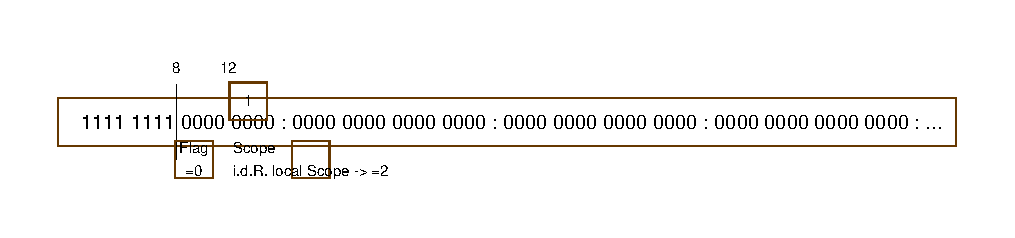
\includegraphics{multicast.pdf}
	\caption{Bit-Einteilung IPv6 Multicast Adresse}
\end{figure}

\textrightarrow\space \textbf{ff02:: /16} 

\textbf{Beispiele:}
\begin{itemize}
    \item ff02::1 \textrightarrow\space All Nodes
    \item ff02::2 \textrightarrow\space All Routers
\end{itemize}


\subsubsection{Neighbor Discovery Protocol (NDP)}

Idee: 2-Schrittverfahren um 'etwas' über das Netz zu erfahren
\begin{enumerate}
    \item Host sendet eine 'Solicitation' (= Aufforderung)
    \item Alle Betroffenen antworten mit einem 'Advertisement' (=Werbung/Anzeige)
\end{enumerate}

Beispiel:
\begin{enumerate}
    \item Host sendet Router Solicitation (=Multicast FF02::2)
    \item Alle Router antworten mit Router Advertisement
\end{enumerate}

\subsubsection{Stateless Address Auto Configuration (SLAAC)}

Prozess um ohne DHCP eine gültige Globale Adresse bekommen.\\
Ablauf:
\begin{enumerate}
    \item Host: RS (Router Solicitation)
    \item Alle Router: RA (Router Advertisement)\\
        \textrightarrow\space Host 'schneidet' vordere 64 Bit von Router IP ab und setzt sie mit seiner Interface ID zusammen
    \item Neue IP wird über DAD (Duplicate Address Detection)\\
    \textrightarrow\space Host hat eine Globale IP!
\end{enumerate}


\subsubsection{DHCPv6}

Weil bei SLAAC die DNS-Option fehlt, brauchen die Hosts aber die DNS-IP!

\textrightarrow\space DHCP Konfigurieren
\begin{itemize}
    \item Stateless DHCP : NDP (zusätzlich Optionen)
    \item Stateful DHCP  : Klassisch
        \begin{enumerate}
            \item Solicitation
            \item Advertisement
            \item (Request)
            \item (Acknowledge)
        \end{enumerate}
\end{itemize}

\subsection{Domain Name System (DNS)}

\subsubsection{Wichtige Begriffe}

\begin{itemize}
    \item FQDN: Fully qualified domain name
    \item WINS: Windows internet name server
    \item NetBIOS: Network basic input/output system
\end{itemize}

\subsubsection{Aufbau FQDN}

\begin{table}[H]
    \centering
    \begin{tabular}{|l|l|l|l|}
         \hline
         www.&tagesschau&.com&.\\\hline
         Host&Second Level Domain& First Level Domain & Root (Wurzel)\\\hline
    \end{tabular}
\end{table}

\textbf{Jede FQDN ist weltweit eindeutig!}

\subsubsection{NetBios Name Auflösung Reihenfolge}
\textbf{Bei H-Knoten:}
\begin{enumerate}
        \item Cache wird überprüft (Cache anzeigen: 'ipconfig -displaydns', Cache lösche: 'ipconfig -flushdns)
	\item Hosts/LMHosts Datei
	\item WINS (über DHCP Option)
        \item Broadcast
\end{enumerate}

\subsubsection{FQDN Auflösung}

\begin{figure}[H]
	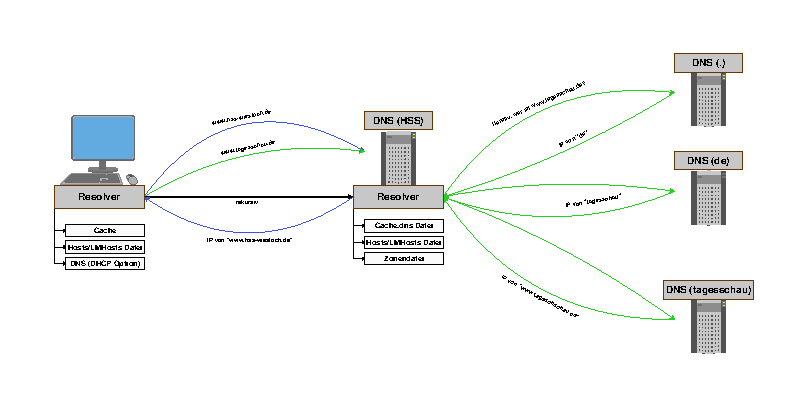
\includegraphics[width=\textwidth]{fqdn.pdf}
	\caption{Ablauf Auflösung FQDN}
\end{figure}


\subsubsection{Zonendatei}

hss-wiesloch.de.dns Datei in win32:\\
Record:

\begin{tabular}{|c|c|c|c|c|}
\hline
    \(<\)Name\(>\)&\(<\)TTL\(>\)&\(<\)Class\(>\)&\(<\)Type\(>\)&\(<\)Data\(>\)\\\hline
    www&Zeit in ms&IN&A&IPv4\\\hline
    www&Zeit in ms&IN&AAAA&IPv6\\\hline
\end{tabular}

		
\textbf{Name der Zonendatei:}
z.B.: www.hss-wiesloch.de = FQDN
\textrightarrow\space DNS \textrightarrow\space Datei: hss-wiesloch.de.dns



\textbf{Typen}:
\begin{itemize}
    \item MX: (Mail)IP v. Mail-Server
    \item SRV: (Service) z.B.: AD-Server
    \item CNAME: Alias (\(<\)name\(>\): lalala \(<\)type\(>\): CNAME \(<\)Data\(>\): www     =\textrightarrow\space lalala.hss-wiesloch.de ist alias für www.hss-wiesloch.de)
    \item NS: Name Server (\(<\)data\(>\): IP v. DNS)
    \item SOA: Start of authority \textrightarrow\space \(<\)data\(>\) enthält den primären DNS
    \item PTR: (PTR = Pointer)\\
    	www.hss-wiesloch.de  zu IP \textrightarrow\space forward lookup\\
    	10.1.2.3 zu name \textrightarrow\space reverse lookup\\
    	\textbf{Inverse}: 3.2.1.10\\
    Name Reverse Zone:\\
    	2.1.10.in-addr.dns\\
    	\begin{tabular}{|c|c|c|c|c|}
                \hline
                \(<\)Name\(>\)&\(<\)TTL\(>\)&\(<\)Class\(>\)&\(<\)Type\(>\)&\(<\)Data\(>\)\\\hline
                3&…&IN&PTR&FQDN: www.hss-wiesloch.de\\\hline
            \end{tabular}
\end{itemize}


\subsubsection{Exkurs: (Datensicherheit) / Ausfallsicherheit}

\textrightarrow\space Redundanz d.h. Datenbank existiert doppelt, dreifach…

\textrightarrow\space Replikation
\begin{enumerate}
    \item Kopie: Master \textrightarrow\space Slave(schreibgeschützt)
	             Primäre Zone \textrightarrow\space Sekundäre Zone
    \item Nur Änderungen: inkrementeller Zonentransfer
Jeder Server: Multimaster-Replikation (z.B. AD)
\end{enumerate}
	

\subsection{Dynamic Host Configuration Protokoll (DHCP)}

DHCP ermöglicht eine automatische Konfiguration von neu ins Netz eingebundenen Geräten.\\
Dabei werden folgende Einstellungen am Gerät konfiguriert:

\begin{itemize}
    \item Eigene IP-Adresse
    \item Netzmaske / Subnetzmaske 
    \item Gateway
    \item DNS
    \item Time- und NTP-Server
\end{itemize}

Ohne DHCP müsste ein Administrator diese Einstellungen für jedes Gerät per Hand vornehmen.

\subsubsection{DHCP Server}
Der DHCP-Server ist ein Hintergrundprozess und wartet auf dem UDP-Port 67 auf die Anfrage eines DHCP-Clients, der sich mit dem Netzwerk verbinden möchte.\\
In einer vorher definierten Konfigurationsdatei befinden sich die erforderlichen Parameter, die dann automatisch zum Client gesendet werden, um diesen zu konfigurieren.

Es gibt drei unterschiedliche Betriebsmodi eines DHCP-Servers:

\begin{enumerate}
    \item \textbf{Manuelle Zuordnung: }Auch als statistisches DHCP bezeichnet. Die am DHCP-Server festgelegten IP-Adressen werden festen MAC-Adressen (der Hardware-Adresse des einzelnen Netzwerkadapters - zur eindeutigen Identifikation des Gerätes) zugeordnet. Die Adressen werden fest vergeben und es ergibt sich der Nachteil, dass keine zusätzlichen Clients in das Netz eingebunden werden können, da die Adressen nur fest vergeben werden. Aus Sicherheitsperspektive kann das aber auch erwünscht sein.
    \item \textbf{Automatische Zuordnung:} Bei dieser Zuordnung wird ein festgelegter Bereich von IP-Adressen durch den DHCP-Server zugeordnet. Sobald die Adressen miteinander verknüpft sind, bleiben auch diese auf unbestimmte Zeit verbunden. Der Nachteil ist, dass neue Clients keine IP-Adresse erhalten, wenn der Bereich komplett vergeben ist.
    \item \textbf{Dynamische Zuordnung:} Im Unterschied zu den beiden vorherigen Verfahren ist bei der dynamischen Zuordnung die Zuordnung zeitlich begrenzt. Heißt, dass der DHCP-Server innerhalb seiner Konfigurationsdatei festlegt, wie lange eine IP-Adresse an einen Client gegeben werden darf. Diese vom Administrator festgelegte Zeit wird in der IT auch als "Lease-Time" (dt. Leihdauer) bezeichnet.
\end{enumerate}



\begin{flushleft}

\section{Hardware}
\subsection{Hardware von Computern}

\subsubsection{Grundfunktionen und Entwicklung}

Computer arbeiten prinzipiell nach dem EVA-Prinzip (\textbf{E}ingabe, \textbf{V}erarbeitung, \textbf{A}usgabe)

\begin{figure}[H]
\begin{center}
  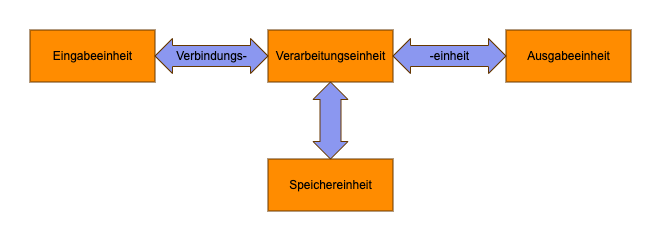
\includegraphics[width=1\textwidth]{EVA-Prinzip.png}
  \end{center}
  \caption{Grafische Darstellung EVA Prinzip}
\end{figure}

\textbf{Exemplarische Hardware:}

\begin{table}[H]
    \centering
    \begin{tabular}{l|l}
        Einheit & Exemplarische Hardware \\\hline
        Eingabeeinheit & Tastatur, Maus, Mikrophon, Scanner \\
        Verarbeitungseinheit & CPU, GPU \\
        Ausgabeeinheit & Monitor, Drucker, Lautsprecher \\
        Speichereinheit & HDD, SSD
    \end{tabular}
\end{table}

Computer werden heutzutage kaum noch als „Stand-alone-Geräte“/“Einzelplatzrechner“ benutzt, sondern sind firmenintern oder weltweit vernetzt. Trotzdem ist die Bezeichnung „PC – Personal Computer“ geblieben. Zusätzlich dazu gibt es noch weitere Bezeichnungen, die verschiedene Geräteklassen bilden:

\begin{longtable}{|p{0.15\textwidth}|p{0.4\textwidth}|p{0.323\textwidth}|}

        \hline
        \textbf{Bezeichnung} & \textbf{Beschreibung} & \textbf{Einsatzzweck}\\\hline
        \textbf{Barebone} & Meist würfelförmiges Gehäuse ca. 20x20x35 cm.
        Meist ist die Bestückung der Barebones nach Kundenwunsch 
        möglich – von extrem sparsam bis zu durchschnittlichen 
        Leistungen alles möglich. & Einsatz als sparsamer Office-Rechner für die tägliche Arbeit bei geringem Platz und Stromverbrauch.\\\hline
        
        \textbf{Notebook} & Mobiles Endgerät bei dem alle Komponenten inkl. Tastatur und Flachbildschirm untergebracht sind. Größe meist 35x28x3 cm. \newline Gutes Preis-Leistungsverhältnis. \newline Hardware sitzt meist „unter“ der Tastatur. & Hoch mobiles arbeiten in verschiedenen Anwendungen – häufig in Verbindung mit Docking-Station um in Büros schnell konfigurierbare und flexible Arbeitsplätze zu schaffen. \\\hline
        
        \textbf{Netbook} & Mobiles Endgerät bei dem alle Komponenten inkl. Tastatur und Flachbildschirm untergebracht sind. Größe meist 25x18x2 cm und damit kleiner als ein Notebook/Laptop. Dafür geringere Leistung als ein Notebook. \newline Hardware sitzt meist „unter“ der Tastatur. & Hoch mobiles Arbeiten, meist in Office-Anwendungen. Mobilität steht noch mehr im Fokus als beim Notebook. Dafür nimmt die Leistung und damit die Fähigkeit zum Einsatz als Büroarbeitsplatz ab. \\\hline

        \textbf{Tablet} & Mobiler PC mit sehr flachem Gehäuse (<2 cm) und integriertem Display (Touch- und Stifteingabe). Meist keine Tastatur (außer bei hybriden Geräten). \newline Hardware sitzt „unter“ dem Display und es sind mobile Betriebssysteme im Einsatz. & Mobiles Arbeiten – selten die Eingabe von Daten, eher das Präsentieren von Informationen beim Kunden (z.B. im Außendienst – Marketing/Verkauf). \newline Sonderfälle wie z.B. Tablets zum Zeichnen und modellieren oder Branchenlösungen (Kassensysteme). \\\hline

        \textbf{Smartphone} & Mobiler PC mit sehr flachem und kleinem Gehäuse und integriertem Display (Touch- und Stifteingabe). Leistungsschwächeres Tablet. & Mobile Kommunikation (z.B. Mails oder Telefonate) bereitstellen. Daten einsehen, jedoch nur selten verarbeiten. \\\hline

        \textbf{Wearable Computer} & tragbare Kleinstcomputer, die direkt am Körper getragen werden. Die meiste Zeit sind sie nur im Hintergrund tätig. Beispiele sind Smartwatches oder Datenbrillen. & Mobile Kommunikation, Überwachung von Körperfunktionen, bereitstellen von Informationen. \\\hline

        \textbf{Desktop-PC} & Flexible Konfiguration der Hardware in allen Facetten möglich. D.h. freie Wahl von Betriebssystem, Hardware und Größe des Gehäuses. \newline Leistungsfähigkeit schwankt stark aufgrund der flexiblen Hardware. \newline Eingabe – und Ausgabegeräte sind nicht fest verbaut, sondern werden über I/O-Schnittstellen angebunden. & Alles, außer mobiles Arbeiten. \newline Je nach Leistung von reiner Office-Tätigkeit bis hin zum rendern oder compilieren von Code ist alles möglich. \\\hline

        \textbf{Industrie-PC} & Speziell für Aufgaben im industriellen Bereich eingesetzt. Verarbeitung von Prozessdaten in Echtzeit steht im Vordergrund (z.B. Überwachung einer Produktionsmaschine). \newline Häufig so ausgelegt, dass sie Temperatur-, Schock- und Wasserresistent sind. & Steuerung und Überwachung von Industrieanlagen.

        \\\hline

\end{longtable}

\break

\subsubsection{Hersteller und Leistungsmerkmale}

\textbf{Das Leistungsportfolio im IT-Bereich}

Die Datenverarbeitung in Unternehmen verfolgt unterschiedliche Ziele und wird unterschiedlich ausgelebt. In einigen Betrieben gilt die Datenverarbeitung als Mittel zum Zweck, in anderen ist sie eine Kernkompetenz und Verkaufsmerkmal.
Je nach Ziel der Datenverarbeitung gilt es, die passende Geräteklasse von einem entsprechenden Hersteller und zur Aufgabe passenden Leistungsmerkmalen anzuschaffen.

\textbf{Ziele der Datenverarbeitung}
\begin{itemize}
    \item   Schneller Verarbeitung großer Datenmengen
    \item   Beseitigung monotoner Routinetätigkeiten
    \item   Verbesserung und Automatisierung der Arbeitsabläufe
    \item   Bessere Individualisierung und Automatisierung durch Entscheidungssysteme, autonome und intelligente Unterstützungssysteme
    \item   Mehr und schnellere Informationen über Vorgänge (besseres Informationssystem)
    \item   Bessere Kommunikation durch die Integration und Vernetzung von Aufgaben und Funktionen
    \item Höhere Wirtschaftlichkeit durch geringere Personal- und Sachkosten
    
\end{itemize}

\begin{longtable}{|l|p{6cm}|p{6cm}|}
    \hline
        \textbf{Geräteklasse} & \textbf{Bekannte Hersteller} & \textbf{Leistungs-/Entscheidungsmerkmale} \\\hline

        \textbf{Barebone} & Intel, Gigabyte, Dell, Fujitsu, Hyundai, HP & Leise/Passive Kühlung (Sone), Preis, Stromverbrauch (Watt), Gehäusegröße, vorgefertigte Konfiguration (Massenbestellungen möglich?), Leistung (Anzahl Kerne; Taktfrequenz von CPU, RAM und ggf. GPU; Speicherplatzmenge RAM, Anzahl Anschlüsse) \\\hline

        \textbf{Desktop-PC} & HP, Dell, Intel, Apple, Medion & Preis, Grafikkartenleistung (VRAM, Taktung), CPU-Leistung (Taktung, Anzahl der Kerne, Overclocking möglich?), RAM, Konnektivität (HDMI/Display Port, USB, Ethernet), Kühlung(Lautstärke; Wasser oder Luft), Speicher (Kapazität, SSD/HDD), Stromverbrauch, Nachrüsten möglich? \\\hline

        \textbf{Notebook/Laptop} & Acer, HP, Dell, Lenovo, Asus, Apple, MSN & Preis, Mobilität/Akkulaufzeit, Konnektivität (Ethernet vorhanden?), Bildschirm (Auflösung, Bildwiederholrate), Grafikkartenleistung (VRAM, Taktung), CPU-Leistung (Taktung, Anzahl der Kerne), RAM, Konnektivität (HDMI/Display Port, USB, Ethernet) \\\hline

        \textbf{Netbook} & Lenovo, Panasonic, Google, Microsoft & Preis, Mobilität/Akkulaufzeit, Konnektivität (Ethernet vorhanden?), Bildschirm (Auflösung, Bildwiederholrate), Grafikkartenleistung (VRAM, Taktung), CPU-Leistung (Taktung, Anzahl der Kerne), RAM, Konnektivität (HDMI/Display Port, USB, Ethernet) \\\hline

        \textbf{Tablet} & Samsung, Apple, Microsoft, Lenovo & Preis, Mobilität/Akku, Bildschirmauflösung, Betriebssystem, Display, Kamera \\\hline 

        \textbf{Smartphone} & Samsung, Apple, OnePlus, Google, Nokia, Huawei, Sony, Blackberry & Preis, Mobilität/Akku (Ladezeiten), Fingerabdrucks Sensor, Design, Konnektivität (AUX?), Betriebssystem, Display, Kamera \\\hline

        \textbf{Industrie-PC} & OnLogic, Siemens, Histton & Preis, Staubschutz, Temperaturbeständigkeit \\\hline

        \textbf{Wearables} & Apple, Samsung, Huawei, Epson, Microsoft, Fossil & Preis, Akkuleistung, Funktionen(Körperfunktionen tracken, Sensoren), Design

        \\\hline
\end{longtable}

\break

\subsubsection{Ergonomie am Arbeitsplatz}

\textbf{Ergonomie} ist eine wissenschaftliche Disziplin, die sich mit der menschlichen Arbeit befasst. Konkret stellt sie sich die Frage, wie ein Arbeitsplatz gestaltet sein muss, um eine perfekte Symbiose aus Menschen und Arbeitsmitteln (hierzu gehören im Übrigen auch Maschinen und Werkzeuge) herzustellen. Auch die Inhalte der Arbeit, das allgemeine Umfeld am Arbeitsplatz und die Organisation sind wichtige Aspekte, die alle ihren Anklang in der Ergonomie finden und berücksichtigt werden müssen. Die Gesundheit – sowohl körperliche als auch geistige – steht in jedem Fall klar im Vordergrund.

Faktoren, die bei der täglichen Arbeit auf eine Person einwirken:
\begin{itemize}
    \item Langes Sitzen und schlechte Körperhaltung
    \item Blaulicht intensive Arbeit am Bildschirm
    \item Ermüdung der Augen durch langes betrachten des Bildschirms
    \item Schlechte oder zu „gute“ Belüftung des Arbeitsplatzes
    \item Lärm am Arbeitsplatz (Nebengeräusche)
    \item Wenig natürliches Licht
    \item Schlechte IT-Ausstattung
    \item Schlechte Ergonomie der Tastatur/Maus
    \item Generell zu lange Verwendung - egal von was
    \item Geräte mit großer Strahlung
    \item Überarbeitung und dadurch Folgeeffekte wie Schlafmangel und schlechte Ernährung
    \item Staub und Feinstaub
\end{itemize}


Möglichkeiten, die Belastung bei der Arbeit am Computer möglichst gering zu halten:

\begin{itemize}
    \item Häufiges Wechseln der Sitzposition
    \item Anlehnen mit dem gesamten Rücken vermeiden – trotzdem aufrecht sitzen
    \item Sitzhöhe so, dass die Füße auf dem Boden stehen, Arme und Beine möglichst im rechten Winkel
    \item Höhenverstellbare Schreibtische (der das Arbeiten im Stehen ermöglicht)
    \item Höhe des Monitors, der obere Rand sollte auf Höhe der Augen sein
    \item Abstand Monitor zum Benutzer (das 1,2-Fache der Diagonale in cm)
    \item Verwendung von Blaulichtfiltern beim Monitor (ggf. auch über das Betriebssystem)
    \item Ggf. Brillen mit Blaulichtfiltern
    \item Soweit wie möglich auf Kontrast achten (wenn möglich: Dark Mode)
    \item Regelmäßige Bildschirmpausen (Aufstehen, Bewegen)
    \item Sport treiben, um die Muskulatur zu stärken
    \item Regelmäßiges lüften oder wenn nichts Anderes möglich ist, Luftfilter verwenden
    \item Gesundes Essen und Trinken
    \item Wenn möglich „Schallarme“ Räume
    \item Grüne Büros (Pflanzen)
    \item Gute Beleuchtung (ggf. mit Lampen, die Sonnenlicht nachbilden – Stichwort Vitamin D)
    \item Gutes Zeitmanagement
    \item Tastatur möglichst ebenerdig und ggf. mit Handballenauflagen
    \item Verwendung von ergonomischen Mäusen und Tastaturen
\end{itemize}

\subsubsection{Green IT und Wirtschaftlichkeit}

\textbf{Green-IT} ist ein Leitbegriff zur Schaffung einer Unternehmenskultur, die IT möglichst umweltschonend beschafft und einsetzt. Entscheidender Grundgedanke der Green-IT ist eine ganzheitliche Betrachtungsweise. Beschaffung, Nutzung, Verwertung und Entsorgung von IT werden als Teil eines zusammenhängenden Kreislaufes verstanden.
Dafür gibt es verschiedene Richtlinien, Nachhaltigkeitskonzepte und jährliche Nachhaltigkeitsberichte.

\textbf{Beispiele für Umwelt- und Prüfzeichen:}

\begin{table}[H]
    \centering
    \begin{tabular}{|p{0.5\textwidth}|p{0.5\textwidth}|}
    \hline
    
    \begin{wrapfigure}{l}{0.25\textwidth}
    
\includegraphics{energystar.png}
    \end{wrapfigure}
    
    Weltweit verbreitet
    Zertifiziert die Energieeffizienz von Hardware
    Stammt aus den USA
    Hersteller können das Siegel nach Anfrage anbringen. Die Einhaltung wird aber zunächst nicht kontrolliert.
    Es erfolgen stichprobenartige Kontrollen.

    &
    
    \begin{wrapfigure}{l}{0.25\textwidth}
    
\includegraphics{tuvrheinland.png}
    \end{wrapfigure}
    
    TÜV Rheinland ist als unabhängiges Prüfunternehmen von der Zentralstelle der Länder für Sicherheitstechnik für die Zertifizierung von vielen Produktgruppen zugelassen.
    Ein zertifiziertes Produkt hat bestimmte Prüfungen des TÜV Rheinland – beispielsweise auf Sicherheit und Qualität – erfolgreich bestanden. 
    
    \\\hline

    \begin{wrapfigure}{l}{0.25\textwidth}
    
\includegraphics{ecolabel.png}
    \end{wrapfigure}

    Europaweit anerkanntes Umweltzeichen für Waren und Dienstleistungen.
    Heute vergeben Prüfinstitute das EU-Ecolabel im Auftrag der Umweltministerien der teilnehmenden europäischen Länder.

    &

    \begin{wrapfigure}{l}{0.25\textwidth}
    
\includegraphics[width=\linewidth]{tco.jpg}
    \end{wrapfigure}

    Zertifikat, dass die Ergonomie und die Produktlebensdauer eines Produktes bewertet.
    Vergeben wird es durch den schwedischen Dachverband der Angestellten- und Beamtengewerkschaft.
    Kontrolle erfolgt Stichprobenartig.

    \\\hline

    \end{tabular}
\end{table}

\break

\textbf{Maßnahmen für verschiedene Aspekte von Green-IT:}
\begin{table}[H]
    \centering
    \begin{tabular}{|p{0.3\textwidth}|p{0.7\textwidth}|}

        \hline
    
        Bedarfsgerechter Einsatz von Hardware und Software prüfen & Einsatz von IT-Hardware (z.B. Rechner und Peripheriegeräten) auf korrekte Dimensionierung prüfen

        \\\hline

        Einsparung Energie und Energiekosten durch effiziente IT-Lösungen & Anschaffung von Energieeffizienten Produkten (Energieeffizienzklasse A)
        \newline Abwärme nutzen?! Z.B. Abwärme von Servern in den „Heizkreislauf“ einspeisen.
        \newline Virtualisierung

        \\\hline

        Beratung, den Lebenszyklus der Geräte zu verlängern, Kosten zu senken, Refurbished IT einzusetzen & Extreme Temperaturen und Umgebungseinflüsse und Leistungsszenarien vermeiden
        \newline Bei der Anschaffung auf zukünftige Performance achten
        \newline Auf Möglichkeiten zum Um-, Nach und Aufrüsten achten
        \newline Hardware im Unternehmen weitergeben (z.B. bei Neuanschaffung alte Geräte an Mitarbeiter geben, die weniger Leistung benötigen)
        \newline Bring Your Own Device (BYOD) prüfen

        \\\hline

        Bedarfsgerechter Betrieb der IT anstelle eines durchlaufenden Betriebs & Auf Standby verzichten, wenn möglich
        \newline PC, Monitor und co in Energiesparmodus und wenn möglich ganz ausschalten
        \newline WLAN über Nacht deaktivieren
        \newline Licht o.ä. an Zeit oder Sonnenstand knüpfen

        \\\hline

        Energie und Kosten durch Virtualisierung sparen & Betriebssysteme, Server und Entwicklungsumgebungen virtualisieren, um Kosten für redundante Systeme zu sparen.

        \\\hline

        Einsatz umweltschonender Verbrauchsmaterialien & Einsatz gebrauchten Geräten
        \newline Auf korrekte Mülltrennung bei der Entsorgung von Elektroschrott achten
        \newline Generell recycelte Produkte kaufen
        \newline So weit wie möglich papierlos arbeiten
        \newline Einsatz von grünem Strom

        \\\hline

        Software auf Nachhaltigkeit prüfen, eventuell Open-Source-Software vorziehen & Open-Source-Software ist häufig anpassbar und kann somit an die eigenen Anforderungen angepasst werden.
        \newline Der Funktionsumfang ist zwar häufig geringer aber kann ausreichend sein und ist meistens mit geringeren Hardwareanforderungen verbunden.
        \newline Die Software wird häufig durch eine große Community unterstützt und kann so auf alten System lauffähig und sicher gehalten
        \newline Bei der Anschaffung von neuer Software (egal ob Open-Source oder gekauft) sollten die Hardwareanforderungen und die Passung mit dem restlichen System beachten werden.

        \\\hline

        Mitarbeiter auffordern, umweltfreundlicher zu kommunizieren & Möglichst auf Papier etc. verzichten.
        \newline Lokale Kommunikationssysteme sollten bevorzugt werden.
        \newline Wenn möglich Dienstreisen durch virtuelle Konferenzen ersetzen.



    \\\hline
    \end{tabular}
\end{table}

\subsubsection{Zentraleinheit, Mainboard, Betriebssystem unterscheiden}

Grundlage eines jeden Computers ist die Zentraleinheit. Sie besteht im engeren Sinne aus dem Mainboard und den direkt darauf bestückten Komponenten. Dazu zählen CPU und RAM.
Da RAM-Speicher flüchtig ist und beim Abschalten des Computers gelöscht wird, wird im ROM (Read-Only-Memory) auf dem Mainboard ein Grundprogramm als Grundbetriebssystem oder BIOS (Basic-Input-Output-System, auch UEFI) gespeichert.

Damit alle Operationen konfliktfrei ablaufen können, wird ein Takt vom auf dem Mainboard liegenden Taktgeber (Clock, CLK) vorgegeben.

Das BIOS führt den Startvorgang aus und ruft das Betriebssystem auf, welches auf einem externen Speicher liegt.
BIOS wird durch das schnellere, leistungsfähigere und mit besserem GUI ausgestattete UEFI (Unified Extensible Firmware Interface) abgelöst. EUFI ist im Gegensatz zum BIOS ein eigenes 64-Bit Betriebssystem, es können also Updates geladen werden.

Je nach Hersteller kann das BIOS/UEFI durch das Drücken der Tasten Entf, F1, F2, F8, F10, ESC, … während des Startvorgangs aufgerufen werden.


\subsubsection{Mainboard}

Das Mainboard ist die Hauptplatine des Computers. Alle Hardwarekomponenten sind auf ihm angebracht oder verbaut.

Abmessungen des Mainboards sind im mobilen Bereich sehr individuell auf das Gerät angepasst, aber folgen für Desktop-PCs im Normalfall dem ATX-Formfaktor (Advanced Technology Extended). Merkmale des \textbf{ATX-Formfaktors}:

\begin{itemize}
    \item Festgelegte Größe
    \item Vorgeschriebene Anordnung von Befestigungslöchern
    \item Board ist in verschiedene Bereiche aufgeteilt, welche eine maximale Höhe vorgegeben haben
    \item Anordnung und Art der Anschlüsse sind genormt
\end{itemize}

\textbf{Komponenten auf dem Mainboard:}
\begin{itemize}
    \item Sockel (physikalische Verbindung zwischen Mainboard und CPU)
    \item Chipsatz (Vermittlung der Daten zwischen Input- und Output-Controller)
    \item IC für das UEFI
    \item Batterie für die Systemuhr (wenn Mainboard vom Strom getrennt)
    \item Steckplätze für RAM
    \item Steckplätze für Erweiterungskarten
    \item Schnittstellenanschlüsse
    \item Anschluss für die Spannungsversorgung
\end{itemize}

\break
\textbf{Begriffserklärungen:}
\begin{table}[H]
    \centering
    \begin{tabular}{|p{0.3\textwidth}|p{0.7\textwidth}|}
        \hline

        \textbf{Begriff} & \textbf{Beschreibung} \\\hline

        \textbf{Schnittstellen}
        \newline (Welche finden sich an einem Mainboard)
        &
        PCI-E, (Reset-, HDD, Power), Audio-Anschlüsse, Display-Port, USB-Ports, E-Sata-Ports, PS2-Ports, VGA, DVI, HDMI, Netzwerkanschlüsse, Firewire

        \\\hline

        \textbf{Chipsatz}
        \newline (Welche Chipsätze sind derzeit für AMD und Intel relevant)
        &
        Das zentrale Element auf einem Motherboard ist der Chipsatz (engl. Chipset). Zwar ist der Hauptprozessor das schlagende Element in einem Computer, aber der Chipsatz sorgt erst dafür, dass die verschiedenen Komponenten miteinander kommunizieren und arbeiten können. Der Chipsatz ist das Bindeglied zwischen den einzelnen Komponenten eines Computers. Egal was in einem Computer passiert, der Chipsatz ist immer daran beteiligt.
        \newline AMD – x570, B550, B550a
        \newline Intel – B460, H470, Z490

        \\\hline

        \textbf{Steckplätze für Erweiterungskarten}
        \newline (Welche Anschlüsse/Standards gibt es derzeit auf Mainboards)
        &
        PCI, PCI-E (x4 bis x16), M.2 (z.B. für SSD), SATA, USB, ggf. RAM-Steckplätze, ggf. PWM-Steckplätze

        \\\hline

        \textbf{SATA-Anschlüsse }
        \newline (was versteht man darunter)
        &
        Serial Advanced Technology Attachment \textrightarrow \space Für Massenspeicher wie Festplatten, SSDs, DVD-Laufwerke, … (600 Mbyte/s)

        \\\hline

        \textbf{Sockel} 
        \newline (welche Sockel sind derzeit in Verwendung)
        &
        AMD: AM4, AM3+, STR4(für Threadripper)
        \newline Intel: LGA1151, LGA1200, LGA1155, LGA1151v2

        \\\hline
    \end{tabular}
\end{table}

\subsubsection{Anschlüsse und deren Verwendung}

\begin{outline}
    \1 PCIe-Steckplatz (PCI-Express)
        \2 Schnelle, Interne Schnittstelle für Erweiterungskarten
        \2 Eignet sich grundsätzlich für die Verbindung mehrerer Server und Baugruppen zu einem Computersystem
        \2 Geeignet für zeitkritische Anwendungen wie Bild- oder Tonwiedergabe
        \2 Sowohl für Kupferleitungen als auch für optische Verbindungen vorgesehen
        \2 PCIe Halbleiterschaltungen werden abgewandelt auch für DisplayPort, SATA und SAS verwendet
        \2 Verfügt über verschiedene Slots (x1, x4, x8 und x16). Dabei stehen die Zahlen für die Anzahl der in dem Slot kaskadierten Lanes
        \2 Grundsätzlich funktionieren kurze Karten auch in langen Slots
        \2 WICHTIG: mechanische Länge sagt nichts über die Anzahl der Lanes eines Slots aus
    \1 SATA (Serial-ATA)
        \2 Schnittstelle zum Anschluss von Massenspeichern
        \2 Blaue SATA-Buchsen sind mit 6 Gbit/s zurzeit die schnellsten
        \2 Ist wie USB abwärtskompatibel
        \2 Rote und Schwarze SATA-Buchsen setzen je nach Hersteller unterschiedliche Spezifikationen um (z.B. RAID-Unterstützung)
    \1 USB (Universal Serial Bus)
        \2 Universelle Schnittstelle für Peripheriegeräte
        \2 Lässt sich durch Steckkarten oder USB-Hubs fast beliebig erweitern
        \2 Identifikation der Geräte wird vom USB-Hostadapter im Computer durchgeführt
        \2 Hot-Plugging und Plug-and-Play möglich
        \2 Abwärtskompatibel
        \2 Zu USB zählt auch Firewire (mittlerweile eher selten verwendet) und Thunderbolt
        \2 Thunderbolt fasst in einer Steckverbindung USB, DisplayPort und PCIe zusammen und erreicht eine Geschwindigkeit von 10, 20 oder 40 Gbits/s
    \1 M.2-Port
        \2 Slot-artige Steckverbindung die für streifenförmige SSDs gedacht ist
        \2 Löst den mSATA-Anschluss ab
    \1 Lüfteranschlüsse
        \2 Entweder 3-Pin Anschlüsse (DC-Control: Kontrolle der Geschwindigkeit über die Spannung) oder 4-Pin Anschlüsse (Kontrolle der Geschwindigkeit mit PWM-Signal auf 4tem Pin)
        
\end{outline}

\subsubsection{CPU Grundlagen}

Der \textbf{Prozessor} bzw. Hauptprozessor (\textbf{CPU} – \textbf{C}entral \textbf{P}rocessing \textbf{U}nit) ist das Kernstück und die zentrale Verbindungseinheit eines Rechners.
Besteht aus mehreren Milliarden Transistoren, die auf einem Mikrochip angebracht sind – wird daher auch \textbf{Mikroprozessor} genannt.
Der eigentliche Mikrochip wird als \textbf{Prozessor-Die} bezeichnet und ist wesentlich kleiner als die Prozessorplatine. Die Größe des Prozessors wird maßgeblich durch die Anzahl der Kontakte bestimmt.

Die CPU holt nacheinander Befehle aus dem Speicher und veranlasst Informationsverarbeitung, Steuerung und Kontrolle der Systeme.

\textbf{Grundlegende Funktionsblöcke einer CPU:}

\begin{table}[H]
    \centering
    \begin{tabular}{|p{0.3\textwidth}|p{0.7\textwidth}|}
        \hline

        \textbf{Instruction Decode Unit (IDU)} & Befehlsdecoder; übersetzt die Befehle, die dem Prozessor als Programm übergeben werden, anhand eines prozessorientierten ROMs in Microcode und übergibt sie der Ausführungseinheit.

        \\\hline

        \textbf{Execution Unit (EXU)} & Ausführungseinheit; führt die im Mikrocode vorliegenden Befehle aus.

        \\\hline

        \textbf{Control Logic (COL)} & Kontrolleinheit; steuert den Ablauf der Mikroprogramme.

        \\\hline

        \textbf{Internal ROM} & Interner ROM-Speicher; beinhaltet die Mikroprogramme des Prozessors

        \\\hline

        \textbf{Bus Interface Logic (BIL)} & Bussteuereinheit; Schnittstelle zwischen den internen Verbindungen und der Verbindung zum Chipsatz.

        \\\hline

        \textbf{Arithmetic Logic Unit (ALU)} & Arithmetisch logische Einheit; führt arithmetische und logische Rechenoperationen aus.

        \\\hline

        \textbf{Floating Point Unit (FPU)} & Fließkomma-Rechner/Co-Prozessor; führt Berechnungen mit Gleitkommazahlen aus.

        \\\hline

        \textbf{Data Cache (DC)} & Cache-Speicher für Daten

        \\\hline

        \textbf{Code Cache (CC)} & Cache-Speicher für Befehle; schneller Zwischenspeicher für Befehle.

        \\\hline
    \end{tabular}
\end{table}

\break

\textbf{Wichtige Begriffe:}
\begin{longtable}{|p{0.3\textwidth}|p{0.7\textwidth}|}
        \hline

        \textbf{AMD} & AMD entwickelt und vertreibt Computerchips, Mikroprozessoren, Chipsätze, Grafikprozessoren (GPUs) und System-on-a-Chip-Lösungen (SoC).
        \newline AMD hat keine eigene Herstellung, sondern vergibt die Produktion an Auftragshersteller.

        \\\hline
        
        \textbf{Intel} & Entwickler und Hersteller von Prozessoren für Desktop, Laptop und Servern. Außerdem Grafikchips und z.B. Desktop-PCs.

        \\\hline

        \textbf{TSMC} & Die Taiwan Semiconductor Manufacturing Company, Limited ist nach Intel und Samsung der weltweit drittgrößte Halbleiterhersteller und der weltweit größte unabhängige Auftragsfertiger für Halbleiterprodukte.

        \\\hline

        \textbf{Prozessorarchitektur} & Unter Architektur versteht man bei Mikroprozessoren das technische Prinzip bzw. das Verfahren, nachdem Daten und Programme verarbeitet werden. Man unterscheidet CISC- und RISC-Prozessoren.CISC – Complex Instruction Set Computing (meist x86-Architekturen) RISC – Reduced Instruction Set Computing (meist ARM-Architekturen)Die Generationen einer CPU wie z.B. Tiger Lake oder Zen 3 können auch als Mikroarchitektur bezeichnet werden. Dabei dreht es sich um den genauen Aufbau einer CPU auf Ebene des Schaltblockplans.

        \\\hline

        \textbf{Strukturgröße} & Bezeichnet die Flächennutzung in Nanometern bei Chips. Derzeit sind 7nm bei AMD und 10-14nm bei Intel in Verwendung. Je kleiner die nm-Angabe ist, desto leistungsstärker und energieeffizienter ist der Chip.

        \\\hline

        \textbf{Cache} & Besonders schneller Zwischenspeicher, der direkt mit der CPU verbunden ist und die CPU durch Speicherung der wartenden Prozesse und Daten entlastet. Es gibt normalerweise 3 Größen L1, L2 und L3-Cache, wobei L1 der kleinste und L3 der größte Speicher ist. L1 befindet sich direkt am Kern (jeder Kern 1 Cache) L3-Cache wird meist zwischen allen Kernen geteilt.

        \\\hline

        \textbf{Taktfrequenz} & Die Taktfrequenz misst die Anzahl der Takte oder Zyklen, die von der CPU pro Sekunde durchgeführt werden in GHz (Gigahertz). Eine CPU mit einer Taktfrequenz von 3,2 GHz führt pro Sekunde 3,2 Milliarden Takte aus. Ganz allgemein lässt sich sagen, dass ein höherer Takt besser ist.

        \\\hline

        \textbf{Parallelisierung} & Parallele Abarbeitung von verschiedenen Befehlen durch z.B. Mehrkernprozessoren (mehrere Rechenkerne auf einer CPU – z.B. Ryzen 5800 hat 8 baugleiche Rechenkerne). Häufig findet man Mehrkernprozessoren in Verbindung mit Multi-Threading (SMT bei AMD und Hyper-Threading bei Intel). Das bedeutet, es werden in einem Kern parallel mehrere Befehle/Programmabläufe (Threads) bearbeitet.

        \\\hline

        \textbf{Turbo Boost / Precision Boost} & Automatische Übertaktung der CPU bzw. einzelner Kerne bei Intel (Turbo) und AMD (Precision). Je nach thermischer und spannungsbedingter Reserve und nach Arbeitslast der restlichen Kerne wird der Takt eines Kerns bis zur maximalen Grenze erhöht, um kurzzeitig die Verarbeitung der Daten zu beschleunigen.

        \\\hline

        \textbf{TDP} & Thermal Design Power – gibt die maximale abgegebene Wärmeleistung eines Prozessors in Watt an. Liegt unter der tatsächlichen Spannung, gibt aber einen Hinweis auf den Verbrauch des Systems. TDP verschiedener Hersteller lassen sich aufgrund unterschiedlicher Messparameter nicht miteinander vergleichen. Neben dem Verbrauch gibt die TDP auch einen Hinweis auf die Dimensionierung des Kühlers. Je größer desto besser sollte das Kühlsystem sein (Passiv, Luft, Wasserkühlung).

        \\\hline

        \textbf{GPGPU} & General Purpose Computation on Graphics Processing Unit – Schnittstelle mit der Möglichkeit, allgemeine Berechnungen auf die GPU auszulagern. Notwendig, bei Systemen, bei der ein Grafikchip in die CPU integriert ist.
        
        \\\hline
\end{longtable}

\subsubsection{CPU Leistungsmerkmale}

\begin{outline}
    \1 CPU-Takt
        \2 Geschwindigkeit, mit der der Prozessor arbeitet
        \2 In Megahertz (MHz) oder Gigahertz (GHz) angegeben
        \2 Frequenz mit der der Prozessor laut Hersteller getaktet ist
    \1 Anzahl der Prozessorkerne
        \2 Durch Mehrkernprozessoren wird die Leistungsfähigkeit gesteigert
        \2 Mehrkernprozessoren bestehen aus zwei oder mehr gleichen Prozessorkernen auf einem einzigen Mikrochip
        \2 Kerne können gleichzeitig unterschiedliche Prozesse abarbeiten oder parallel einen einzigen Prozess ausführen
        \2 Kerne haben ihren eigenen Takt
        \2 \textrightarrow Weitere Merkmale: Takt des einzelnen Kerns und maximale Taktrate aller Kerne zusammen („All-Core-Boost“)
    \1 Geschwindigkeit, mit der Daten zum Prozessor übertragen werden
        \2 Abhängig von Taktung und Verbindungsart der Datenleitung
        \2 Es existieren verschiedene Varianten (Front Side Bus, QuickPathInterconnect, HyperTransport, Direct Media Interface, Unified Media Interface)
    \1 MIPS
        \2 \textbf{M}illions of \textbf{I}nstructions \textbf{p}er \textbf{S}econds
    \1 FLOPS
        \2 \textbf{F}loating \textbf{P}oint \textbf{O}perations \textbf{P}er \textbf{S}econd
        \2 Misst Leistungsfähigkeit anhand der Gleitkommazahlen-Operationen, die in einer Sekunde ausgeführt werden können
    \1 CISC
        \2 \textbf{C}omplex \textbf{I}nstruction \textbf{S}et \textbf{C}omputing
        \2 Häufig Bezeichnung für allround-Prozessoren, die einen komplexen Befehlssatz verarbeiten können
        \2 Bearbeitung eines Befehls kann mehrere Takte dauern, da ein komplexer Befehl aus mehreren kleinen Befehlen bestehen kann

\break
\break

    \1 RISC
        \2 \textbf{R}educed \textbf{I}nstruction \textbf{S}et \textbf{C}omputer
        \2 Kleinerer und effizienterer Befehlssatz
        \2 Meistens ein Befehl pro Takt
        \2 Aufgaben können effizienter und kleinschrittiger abgearbeitet werden
    \1 SIMD
        \2 \textbf{S}ingle \textbf{I}nstruction, \textbf{m}ultiple \textbf{d}ata; Rechnerarchitektur mit Vektorprozessoren, bei der viele Prozessoren ihre Befehle von einem Befehlsprozessor erhalten und gleichzeitig unterschiedliche Daten verarbeiten
    \1 Simultaneous Multithreading (SMT) / Hyper-Threading (HT)
        \2 SMT: Prozessor kann mehrere Threads gleichzeitig ausführen
        \2 HT: Intel SMT
    \1 Cachegröße
        \2 Für Effizienz des Cache ist Größe (je größer, desto besser) und Taktfrequenz entscheidend
    \1 Speicherbusse
        \2 Anzahl und Datenrate der unterstützten Speicherbusse – umso höher, desto besser
    \1 Befehlssatzerweiterung
        \2 Erweiterung des klassischen Befehlssatzes, der zusätzliche Befehle hinzufügt
        \2 Kann Leistungsfähigkeit erhöhen
\end{outline}

\textbf{CPU-Taktsteigerung:}
\begin{outline}
    \1 Eine CPU-Taktsteigerung (z.B. durch Boost-Funktionen oder Übertaktung) führt in der Regel zwar zu einer höheren Verarbeitungsgeschwindigkeit, allerdings steigt auch die Verlustleistung in Form von Wärme, die abgeführt werden muss. Dies liegt daran, dass für die Erhöhung der Taktrate meist auch die am CPU anliegende Spannung (Corespannung) erhöht werden muss. Das UEFI stellt die Corespannung in der Regel automatisch ein und überwacht diese im laufenden Betrieb. Je nach Energiespartechnik oder gewünschter Leistung wird die Spannung lastabhängig gesteuert oder einzelne Kerne komplett abgeschaltet.
    
    \1 Eine niedrigere Corespannung verringert die Leistungsaufnahme und die Abwärme einer CPU und ermöglicht dadurch höhere CPU-Taktraten.

    \1 Die Corespannung ist ab Werk auf eine „sichere“ Einstellung festgelegt, die für jeden Nutzer ausreichend ist. Sie kann manuell erhöht oder gesenkt werden, um z.B. den CPU zu übertakten oder die Leistungsaufnahme zu optimieren (undervolting).
\end{outline}

\textbf{Weitere wichtige Begriffe}
\begin{outline}
    \1 x64 und ARM sind die häufigsten Arten von Prozessoren
        \2 x64 \textrightarrow\space CISC \textrightarrow\space zielt auf höhere Leistung
        \2 ARM \textrightarrow\space RISC \textrightarrow\space zielt auf höhere Energieeffizienz
    \1 EIST-Verfahren
        \2 Enhanced Intel SpeedStep Technology
        \2 Energiesparfunktion von Intel, bei der Takt und Kernspannung dynamisch angepasst werden
        \2 Besonders relevant auch für Notebooks, da erkannt wird ob Betrieb per Akku oder Netzteil stattfindet
        \2 AMD Gegenstück heißt CoolnQuiet
\end{outline}

\subsubsection{RAM}

\begin{outline}
    \1 Random Access Memory
    \1 Wird auch als \textbf{Lese-Schreibspeicher oder Arbeitsspeicher} bezeichnet
    \1 Wird beim Herunterfahren des Endgerätes gelöscht \textrightarrow\space flüchtiger Speicher
    \1 Es wird zwischen \textbf{SRAM} und \textbf{DRAM} unterschieden	
    \1 SRAM (Static Random Access Memory):
        \2 Speicherzellen aus Flipflops aufgebaut
        \2 Jedes Flipflop besteht aus sechs Transistoren und kann entweder 0 oder 1 als Zustand einnehmen
        \2 Durch einen kurzen Spannungsimpuls wird er Zustand eingenommen und unverändert gehalten, solange die Betriebsspannung anliegt
        \2 Sehr performant, kürzere Zugriffszeiten als bei DRAM
        \2 Höherer Platzverbrauch durch Flipflops \textrightarrow\space geringe Integrationsdichte (Speichereinheiten pro Flächeneinheit)
        \2 Teurer als DRAM 
        \2 Wird für Cache-Speicher verwendet
    \1 DRAM (Dynamic Random Access Memory)
        \2 Überbegriff für alle dynamisch arbeitenden RAM-Bausteine
        \2 DRAM-Speicherzelle besteht typischerweise aus einem Transistor und einem Kondensator
        \2 Informationsspeicherung erfolgt durch Speichern einer Ladung im Kondensator
        \2 Da Ladung im Kondensator flüchtig ist, muss der Speicher regelmäßig aktualisiert werden (\textbf{refresh}), z.B. alle 32ms
        \2 DRAM ist günstiger und hat höhere Integrationsdichte
        \2 Wird als primärer Arbeitsspeicher eines PCs verwendet
    \1 DDR-SDRAM
        \2 Synchronous Dynamic Random Access Memory
        \2 Heutzutage in PCs verbaut
        \2 Daten werden synchron zum Speicher-Bus übertragen
        \2 Takt wird durch System-Bus vorgegeben
        \2 DDR: Double Data Rate \textrightarrow\space Daten werden im Vergleich zu SD-RAM doppelt so schnell übertragen, da sowohl bei ansteigender als auch bei abfallender Taktflanke übertragen wird (SD-RAM nur bei abfallender)
    \1 Verschiedene RAM-Typen je nach Anwendungsgebiet
        \2 Z.B.: DDR-3, DDR-4, DDR-5, GDDR
        \2 Unterscheiden sich durch maximale Taktraten, Aufbau und Datenübertragungsraten
        \2 DDR4: verbreitetste Variante
        \2 DDR5: Wird immer populärer, noch eher neue Technologie
        \2 GDDR: Ausschließlich verwendet im Grafikbereich (z.B. bei Grafikkarten)
        \2 \textbf{Verschiedene RAM-Typen sind untereinander nicht kompatibel!}
    \1 Formfaktoren
        \2 Man unterscheidet zwischen \textbf{Single-Sided-} und \textbf{Double-Sided-Modulen} (einseitig oder zweiseitig bestückt)
        \2 Größe und Anzahl der Kontakte sind je nach Aufbau und verwendeter Technologie unterschiedlich, aber sind durch \textbf{JEDEC} (Joint Electronic Device Engineering Council) festgelegt und für Hersteller einheitlich
        \2 Im Normalfall werden in Desktop-PCs \textbf{DIMM}-RAM (Dual Inline Memory Modul) Module verbaut. Anschlusskontakte beidseitig am Rand der Leiterplatte angebracht
        \2 Für Laptops oder kleine Computer gibt es SO-DIMM-RAM-Riegel. Das sind kleinere DIMM-RAM Module
    \1 Speicherorganisation
        \2 Unabhängig vom Formfaktor kann der Speicher unterschiedlich organisiert sein:
            \3 Ohne Paritätsprüfung
            \3 Mit Paritätsprüfung
            \3 Mit Fehlerkorrekturcode (ECC – Error Correction Code)
        \2 Paritätsprüfung erlaubt Fehlerkontrolle aber keine Fehlerkorrektur
        \2 Zu acht Datenbits wird zusätzlich ein Paritätsbit benötigt
        \2 Paritätsbit:
            \3 Bezieht sich auf die vorherigen acht Bits
            \3 Even-parity: Die Anzahl der auftretenden 1-Bits wird durch das Paritätsbit zu einer \textbf{geraden} Anzahl ergänzt
            \3 Odd-parity: Die Anzahl der auftretenden 1-Bits wird durch das Paritätsbit zu einer \textbf{ungeraden} Anzahl ergänzt
        \2 Fehlerkorrektur ist nur möglich mit entsprechendem Fehlerkorrekturcode der durch spezielle Algorithmen eine Fehlerorterkennung vornimmt.
        \2 Fehlerkorrekturcodes werden in erster Linie bei High-End-PCs und Servern verwendet
    \1 Speichertiming
        \2 Die Zugriffszeiten auf RAM-Speicherzellen werden durch verschiedene Faktoren beeinflusst. Für RAM-Speicherzellen können vier verschiedene Speichertimings angegeben werden
        \2 1.: tCl: CAS Latency
        \2 2.: tRCD: RAS to CAS Latency
        \2 3.: tRP: Row Precharge Delay
        \2 4.: tRAS: Row Active Strobe
        \2 Generell gilt: je Kleiner/kürzer das Timing und umso mehr MHz, desto besser
\end{outline}

\break

\subsubsection{Netzteile}

Das Netzteil (PSU – Power Supply Unit) versorgt Komponenten des Computers mit Strom. Dazu wird der Wechselstrom aus der Steckdose in niedrigere Gleichspannung umgewandelt.

Je nach Anforderung werden Netzteile von 120 Watt bis 1800 Watt angeboten. Standartrechner brauchen ca. 300 Watt, Gaming- und Profirechner bis zu 1000 Watt.

Minderwertige Netzteile können die daran angeschlossenen Endgeräte beschädigen.

\textbf{80-Plus Zertifikate (Angabe: Benötige Effizienz in \% für Zertifikat):}

\begin{figure}[H]
    \centering
    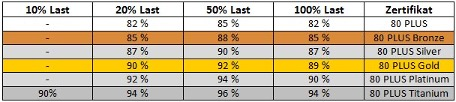
\includegraphics{80plus.jpg}
    \caption{Bedeutung 80-Plus Zertifikate}
\end{figure}

\textbf{Effizienz:}
Effizienz (oder Wirkungsgrad) gibt an, wie viel des verbrauchten Stroms tatsächlich dem Computer zur Verfügung steht.


\subsubsection{Speichermedien}

\begin{outline}
    \1 HDD
        \2 \textbf{H}ard \textbf{D}isk \textbf{D}rive
        \2 Daten werden magnetisch auf sich drehenden Platten gespeichert
        \2 Bestehen aus dem zu beschreibendem Medium, einem Schrittmotor und einem am Zugriffsarm befestigten Lese- und Schreibkopf
        \2 Üblicherweise in 2,5 Zoll (Für Notebooks) und 3,5 Zoll (für Desktop Rechner) verfügbar
        \2 Anschluss mit SATA-Kabel für Datenversorgung und SATA-Kabel für Stromversorgung
        \2 Sollten nicht dauerhaft einem starken magnetischen Feld ausgesetzt werden
        \2 Da die Platte in der HDD sehr schnell rotiert (bis zu 10000 rpm) sollte die vorgeschriebene Einbaulage beachtet werden
        \2 Reagiert empfindlich auf mechanische Einflüsse, daher sollten Erschütterungen vermieden werden
    \1 SSD
        \2 \textbf{S}olid \textbf{S}tate \textbf{D}rive
        \2 Daten werden auf Halbleiterchips gespeichert
        \2 Arbeitet ohne bewegliche Teile
        \2 Unempfindlich gegenüber mechanischen Stößen
        \2 Wesentlich höhere Lese- und Schreibraten als bei HDD möglich
        \2 Gängige Formate: 2,5 Zoll, M.2
        \2 Anbindung über SATA, PCI oder NVMe (PCI-Variante)
\end{outline}

\textbf{Fachbegriffe und Spezifikationen:}

\begin{table}[H]
    \begin{tabular}{|p{0.3\textwidth}|p{0.7\textwidth}|}
        \hline
    
        \textbf{Bauformen} & 1,8 Zoll (selten – bei SSDs), 2,5-Zoll (SSD), 3,5 Zoll (HDD)
    
        \\\hline
    
        \textbf{Festplattenperformance} & Abhängig von den Zugriffszeiten, Datentransferrate und der Leistung der Schnittstelle. Bei HDDs außerdem Latenzen des Lese- und Schreibkopfes und die RPM der Festplatte relevant.
        \newline\textrightarrow\space Details siehe Aufgaben!
    
        \\\hline
    
        \textbf{Umdrehungsgeschwindigkeiten} & Gibt an, wie schnell sich die Platte einer HDD maximal dreht. Angabe in RPM zwischen 5400 und 10000.
    
        \\\hline
    
        \textbf{Datentransferrate} & Hierfür sind die interne Anschlussweise (PCI-E oder SATA) und die Art der Festplatte entscheidend.
    
        \\\hline
    
        \textbf{Cache} & Wie CPUs verfügen Festplatten über hoch performante Zwischenspeicher um Vorgänge wie das Entpacken oder Kopieren von Dateien zu beschleunigen.
        \newline Bei normalen Festplatten sind 16 bis 64 MB-Cache ausreichend. Bei hohen Leistungsanforderungen sollten es 64 bis 128 MB sein. 
    
        \\\hline
    
        \textbf{Self-Monitoring, Analysis and Reporting Technology (SMART bzw. S.M.A.R.T.)} & Industriestandard zur Überwachung von Festplattenlaufwerken (HDD) und Solid-State-Drives (SSD) und dient der Vorhersage eines möglichen Ausfalls des Speichermediums. Es werden dabei die Werte verschiedener Sensoren mit Hilfe von unterschiedlichen Parametern ausgewertet.
    
       \\\hline 
    \end{tabular}
\end{table}

\textbf{Pro und Contra – SSD und HDD}

\begin{table}[H]
    \centering
    \begin{tabular}{|p{0.2\textwidth}|p{0.25\textwidth}|p{0.25\textwidth}|p{0.25\textwidth}|}
         \hline
         & Pro & Contra & Einsatzzwecke \\\hline
         HDD &
         Günstiger als SSD
        \newline Mehr Speicherplatz möglich
        \newline Bessere Möglichkeit zur Datenwiederherstellung
        &
        Langsamer als SSD
        \newline Können laut werde
        \newline Anfällig gegenüber mechanischen Einwirkungen von außen
        \newline Höherer Stromverbrauch
        &
        Langfristigere Datenhaltung ohne Zugriffe (SSDs verlieren nach einer bestimmten Zeit ohne Strom ihre Daten)
        \newline Große Datenmengen speichern
        \newline Viele Lese-/Schreibzugriffe

        \\\hline

        SSD &
        Keine mechanischen Teile \textrightarrow\space robuster, geräuschlos
        \newline Schnell
        \newline Leicht
        \newline Effizient/Geringer Energiebedarf
        &
        Kosten
        \newline Nicht so viel Speicherplatz möglich
        \newline Schlechte Datenwiederherstellungsmöglichkeiten als bei einer HDD
        &
        Mobile Geräte
        \newline Vorteilhaft, wenn schnelle Zugriffszeiten relevant sind (z.B. Betriebssysteme oder Anwendungen, die häufig verwendet werden müssen)

         \\\hline
    \end{tabular}
\end{table}

\subsubsection{Dateisysteme und Formatierung}

Um auf einem Laufwerk Daten zu speichern, muss es zuerst formatiert werden. Dabei werden Strukturen geschaffen, die es dem Betriebssystem ermöglichen Daten auf dem Träger zu verwalten.

Bei Festplatten gibt es folgende Formatierungsschritte:
\begin{enumerate}
    \item Low-Level-Formatierung – LFF 
    \item Erzeugung von Partitionen
    \item Logische Formatierung der Partitionen
Häufig meint „Formatieren“ nur den letzten Schritt.
\end{enumerate}


\textbf{Low Level Formatierung bei HDDs:}
\begin{outline}
    \1 Erfolgt meist durch den Hersteller
    \1 Es werden auf die Plattenoberfläche eine Struktur aus logischen Spuren (tracks) und Sektoren (sectors) geschaffen
    \1 Die Anzahl der Spuren ist abhängig vom physikalischen Aufbau der Platte und sollte nachträglich nur von erfahrenen Usern mit speziellen Programmen geändert werden
    \1 Eine Spur ist ein schmaler, ringförmiger Streifen auf dem später die Daten gespeichert werden
    \1 Die Spuren werden auf jeder Plattenseite bei Spur null beginnend durchnummeriert
    \1 Spuren der gleichen Spurnummer gehören zu einem Zylinder
    \1 Jede Spur ist in Sektoren unterteilt. Sektoren sind die kleinste mögliche Speichereinheit einer Festplatte
    \1 Mehrere Sektoren ergeben zusammen ein Cluster
    \1 Ein Cluster ist der kleinste Speicherbereich eines Dateisystems
\end{outline}

\textbf{Aufbau bei SSDs:}
\begin{outline}
    \1 Für NAND-SSDs gelten folgende Zurechnungseinheiten:
    \2 Cells \textrightarrow\space Pages \textrightarrow\space Blocks \textrightarrow\space Planes
    \1 Ein Block ist die kleinste Struktur, die bei einer SSD gelöscht werden kann.
    \1 Anstelle der LLF gibt es bei SSDs das \textbf{Secure Erase}
    \1 Beim Secure Erase werden alle Bits der Speicherzellen auf 0 gesetzt
\end{outline}


\textbf{Partitionierung}
Eine Partition ist ein logisch selbständiger Teil einer Festplatte, der wie eine physisch separate Einheit funktioniert, vom Betriebssystem aus separates Laufwerk angesprochen wird und sich durch ein Dateisystem nutzen lässt.

Vorteile von Partitionierung:
\begin{outline}
    \1 Einfachere Organisation
    \1 Partitionen können einzeln formatiert werden
    \1 Betriebssystem kann einfach neu installiert werden
    \1 Mehrere Betriebssysteme möglich
    \1 Effizientere Suche nach Dateien
    \1 Einfachere logische Formatierung (z.B. verschiedene Dateisysteme)
\end{outline}

Nachteile von Partitionierung:
\begin{outline}
    \1 Ggf. Verschwendung von Speicherplatz
    \1 Falsches Gefühl von Sicherheit (Ausfall der Festplatte, Viren, etc.)
    \1 Unübersichtlich bei großer Anzahl von Partitionen
    \1 Kopieren/Verschieben von Dateien über Partitionen hinweg relativ langsam
\end{outline}

\subsubsection{Erweiterungskarten}
Viele Funktionen, die früher nur mit zusätzlichen Erweiterungen nachrüstbar waren sind heute auf dem Mainboard implementiert (z.B. Sound-, oder Netzwerkfunktionen). Das Nachrüsten mit zusätzlichen Karten ist daher nur dann erforderlich, wenn man beispielsweise eine qualitativ bessere Leistung erzielen möchte oder besondere Funktionen benötigt.

Der Anschluss von Erweiterungskarten erfolgt meist über einen PCIe-Slot auf dem Mainboard.

\subsubsection{Peripheriegeräte}
Peripherie-Geräte sind alle Geräte, die nach dem EVA-Prinzip zur Ein- und Ausgabe der Daten genutzt werden. Zu den gängigen Peripherie-Geräten gehören unter anderem:
\begin{outline}
    \1 Tastatur
    \1 Maus
    \1 Bildschirm
    \1 Lautsprecher/Headset
    \1 Drucker/Scanner
\end{outline}

\textbf{Eingabeeinheiten}
Tastatur und Maus gehören zu den klassischen Eingabeeinheiten. Bei der Anschaffung sollte auf Ergonomie und die nötigen Rahmenbedingungen geachtet werden.

Neben den klassischen Eingabeeinheiten gibt es außerdem unterschiedliche Branchenlösungen wie Zeichen-Tablets oder 3D Scanner.

\textbf{Ausgabeeinheiten – zentrale Einheit ist der Bildschirm}
Der Monitor ist die wichtigste Ausgabeeinheit.

Heutige Bildschirme werden als Liquid-Crystal-Displays (LCD) angeboten. Hersteller setzten bei LCD-Monitoren auf LED-Technik, da sie sehr energiesparend ist und die LEDs eine Hintergrundbeleuchtung er-möglichen.

Als Standardgröße und normale Eigenschaften für Office-Monitore gelten häufig 27-Zoll, Full-HD, eine Reaktionszeit von 4-8 ms und 60 Hz.

\textbf{Eigenschaften im Überblick}
\begin{longtable}{|p{.2\textwidth}|p{.8\textwidth}|}
    \hline
    \textbf{LCD-Technologie}&
    LCD ist die derzeitige Bautechnologie von Monitoren, die spezielle Verarbeitungsart Thin-Film-Transistor-Technologie (TFT) bei LCD-Monitoren liegt auch LCD-Fernsehern zugrunde.
    
    Flüssigkristalle eines LCD-Monitors bilden die einzelnen Bildpunkte (Pixel) des Monitors. Ein Pixel besteht aus drei Farbfiltern (Rot, Grün, Blau), die rückseitig beleuchtet werden. Die Art der Lichtpolarisation durch die Kristalle unterscheidet sich jedoch nach den Panel-Typen.
    \begin{outline}
        \1 TN: preisgünstig und schnelle Reaktionszeit, relativ energiesparsam, aber schlechte Blickwinkeldichte.
        \1 VA: gute Bildqualität aber geringe Reaktionszeit
        \1 IPS: sehr gute Bildqualität und gute Blickwinkeldichte aber höhere Anschaffungskosten   
    \end{outline}
    \\\hline

    \textbf{Größen / Seitenverhältnis}&
    Größenangaben erfolgen in Zoll (Bildschirmdiagonale), typisch sind 24 oder 27 Zoll bei einem Seitenverhältnis von 16:9. Curved-Bildschirme sind dagegen häufig etwas größer und sind auch im 21:9 Seitenverhältnis zu kaufen.
    \\\hline

    \textbf{Ergonomie}&
    Da Monitore häufig über längere Zeiträume hinweg den zentralen Punkt eines Arbeitsplatzes bilden, ist die ergonomische Ausrichtung von hoher Wichtigkeit.
    
    Eine Rolle spielt neben der Größe, dem dazu passenden Abstand vom Monitor (Diagonale * 1,6) und der Krümmung des Monitors auch die Eigenschaft den Monitor horizontal zu neigen (Tilt), vertikal zu drehen (Swivel) oder horizontal zu drehen bzw. die Höhe zu verstellen (Pivot).
    
    Dazu gibt es außerdem noch verschiedene Filter (z.B. Blaufilter) die die Augen vor einer Ermüdung schützen sollen.
    \\\hline

    \textbf{Reaktionszeit}&
    Die Reaktionszeit beim Monitor gibt an wie viel Zeit die Pixel des Displays benötigen, um einen Farbwechsel vorzunehmen. Üblicherweise wird ein Farbwechsel zwischen zwei Grautönen (Grey to Grey) oder Schwarz und Weiß gemessen. Typisch sind Zeiten unter 10 ms wobei gilt, kleiner desto besser.
    \\\hline

    \textbf{Bildwiederhol-}\\\textbf{frequenz}&
    Gibt an, wie viele Einzelbilder (Refresh) pro Sekunde vom Monitor dargestellt wer-den können. Die meisten Monitore liefern eine Bildwiederholfrequenz von 60 Hz. Das bedeutet, dass pro Sekunde 60 Einzelbilder vom Monitor dargestellt werden können. Daneben gibt es z.B. auch 75, 120 oder 144 Hz. Die treusten Monitore haben bis zu 240 hz.
    \\\hline

    \textbf{Auflösung}&
    Richtet sich nach der Größe und dem Seitenverhältnis eines Monitors.

    Gängig sind 1920 x 1080 (HD), 2560 x 1440 (WQHD) oder 4.096 x 2.160 Pixeln (4k).

    \\\hline
\end{longtable}

\textbf{Ausgabeeinheiten – Drucker unterscheiden}

\begin{longtable}{|p{.3\textwidth}|p{.7\textwidth}|}
    \hline
    
    \textbf{Arbeitsplatz/Desktop Drucker}&
    Werden häufig im kleineren Rahmen im geschäftlichen Bereich eingesetzt. Häufig werden nur einzelne/wenige Arbeitsplätze direkt angebunden um Weg/Zeit zu sparen.

    Häufig handelt es sich um Multifunktionsgeräte mit Drucker/Scanner/Kopierer/Fax.
    \\\hline

    \textbf{Abteilungsdrucker}&
    Für größere Druckvolumen oder Spezialaufträge werden gerne Abteilungsdrucker eingesetzt. Diese sind auf 10000 Ausdrucke und mehr im Monat ausgelegt und bieten den Druck schnell und günstig.
    
    Außerdem können solche Geräte bspw. im Duplex-Verfahren (Beidseitig) drucken und verfügen ebenfalls über Kopie/Scan/Fax Optionen.
    
    Häufig ist die Anmeldung über eine Codekarte oder einen Login notwendig.
    \\\hline

    \textbf{Mobile Drucker}&
    Mobile Drucker sind besonders für Mitarbeiter im Außendienst relevant. Der Druck ist langsam und teuer, dafür sind die Drucker sehr mobil, um bspw. Rechnungen direkt drucken zu können.
    
    
    \\\hline
\end{longtable}
\break
\textbf{Drucksysteme im Vergleich}

Tinten- oder Inkjet-Drucker:
\begin{table}[H]
    \begin{tabular}{|p{.5\textwidth}|p{.5\textwidth}|}
         \hline
         Vorteile & Nachteile
         \\\hline
        
         \begin{outline}
            \1 Druckt auf CDs/DVDs, Spezialpapier.
            \1 Fotodrucke haben hervorragende Qualität.
            \1 Es gibt spezielle Tintenstrahldrucker, mit speziellen Fotofarben.
            \1 Keine Aufwärmphase notwendig.
            \1 Keine Hitzeabgabe.
            \1 Im Betrieb (und vor allem auch Stand-By) leiser.
            \1 Günstigere Anschaffungskosten.
            \1 Geringerer Stromverbrauch.
            \1 Keine Feinstaubbelastung.
            \1 Eher für Wenigdrucker geeignet (unter 200 Seiten pro Monat)
         \end{outline}
         &
         \begin{outline}
            \1 Kürzere Lebensdauer.
            \1 Benötigt hochwertiges (und teures) Druckerpapier.
            \1 Druckpatronen sind sehr teuer.
            \1 Tintenpatronen/Druckkopf trocknen nach längerer Zeit ohne Benutzung ein.
            \1 Spülen mit teurer Druckertinte erhöht die Druckkosten noch zusätzlich. 
            \1 Niedrigere Druckgeschwindigkeit.
            \1 Ausdrucke aufgrund von schlechter UV-Beständigkeit und fehlender Feuchtigkeitsresistenz nicht so lange haltbar.
         \end{outline}
         \\\hline
    \end{tabular}
\end{table}


Laserdrucker:
\begin{table}[H]
    \begin{tabular}{|p{.5\textwidth}|p{.5\textwidth}|}
         \hline
         Vorteile & Nachteile
         \\\hline
        
         \begin{outline}
            \1 Geringe Kosten pro gedruckter Seite.
            \1 Höhere Druckgeschwindigkeit.
            \1 Gut geeignet für Textdrucke wie Dokumente und E-Mails.
            \1 Nicht so anspruchsvoll bezüglich der Papierqualität, es kann z. B. günstiges (und umweltschonendes) Recyclingpapier verwendet werden.
            \1 Hohe Schriftrandschärfe (= scharfe und klare Textausdrucke).
            \1 Hohe Farbtiefe.
            \1 UV- und Feuchtigkeitsresistent. Damit wischfest und es kommt nicht zum Ausbleichen.
            \1 Vor allem für Vieldrucker (Büro und Firmen) geeignet. Rechnet sich ab ca. 200 gedruckten Seiten pro Monat.

         \end{outline}
         &
         \begin{outline}
            \1 Geringe Druckschärfe und deshalb nicht geeignet für das Drucken von Bildern und Fotos.
            \1 Höherer Anschaffungspreis als Tintenstrahldrucker.
            \1 Höhere Schadstoff- / Feinstaubemissionen.
            \1 Benötigt Zeit zum Aufwärmen.
            \1 Wärme- und Geräuschentwicklung.
            \1 Höherer Stromverbrauch.
         \end{outline}
         \\\hline
    \end{tabular}
\end{table}


\subsection{Dateisicherung - für ASP1 wahrscheinlich nur oberflächlich}

\subsubsection{RAID-Systeme}

Bei einem RAID-System handelt es sich um einen logischen Zusammenschluss mehrerer einzelner physischer Massenspeicher, wie z.B. HDD oder SSD Festplatten. In der Regel erreicht man dadurch eine Steigerung der Geschwindigkeit der Schreib- und Lesezugriffe oder die Verbesserung der Datensicherheit.

Ein RAID kommt also immer dann zum Einsatz, wenn folgende Ziele erreicht werden sollen:
\begin{itemize}
    \item durch Datenredundanz die Ausfallsicherheit und damit Datensicherheit verbessern.
    \item durch die Steigerung der Transferraten die Geschwindigkeit (Performance) steigern.
    \item oder beides zusammen.
\end{itemize}



\subsubsection{Backup Verfahren}

Bei einem Backup wird die Sicherheit der Daten durch das Anlegen einer separaten, unabhängigen Kopie erhöht. Bei einem Verlust der Originaldaten kann man auf die Kopie zugreifen und die Daten somit wieder-herstellen. Hierdurch hilft ein Backup auch in solchen Situationen, in denen ein RAID System versagt.

\textbf{Verschiedene Backup Verfahren:}
\begin{outline}
    \1 Inkrementelles Backup
    \1 Differentielles Backup
    \1 Vollbackup
\end{outline}

Die optimale Backup-Methode muss je nach Anwendungsfall gewählt werden. Häufig macht eine Kombination aus allen drei Methoden am meisten Sinn. Zum Beispiel kann ein wöchentliches Vollbackup erfolgen und zusätzlich jeden Tag ein inkrementelles Backup, um das Datenaufkommen niedrig zu halten und mit den entsprechenden Sicherungen die Daten schnell und zu verschiedenen Zeitpunkten wiederherzustellen.


\subsubsection{USV}

Eine USV ist ein Gerät, welches zwischen den Netzanschluss und den oder die Verbraucher geschaltet wird. Sie beinhaltet eine Pufferbatterie und kann daraus Strom liefern, wenn die Netzversorgung ausfällt.


\break

\section{ITS Weiss - Zweites Schuljahr}



\subsection{WLAN}
\subsubsection{Funknetze zur Datenübertragung}

Während für Ethernet Token Ring auf Leitungen wie Kupfer- oder Lichtwellenleiter eingesetzt werden kann, kommen in den letzten Jahren vermehrt Funkstrecken als Übertragungsmedium zum Einsatz.

\textbf{Vorteile:}
\begin{itemize}
    \item Oft das einzig mögliche Medium (z.B. in historischen Gebäuden)
    \item Vergleichsweise unempfindlich gegen Katastrophen (z.B. Erdbeben)
    \item Hohe Mobilität von Nutzern und Stationen
\end{itemize}

\textbf{Nachteile:}
\begin{itemize}
    \item Verschlüsselung erforderlich
    \item Niedrigere Geschwindigkeit (im Durchschnitt)
    \item Geteiltes Medium aller Nutzer \textrightarrow\space beschränkte Bandbreite
\end{itemize}

\textbf{Beispiele:}
\begin{itemize}
    \item WLAN nach IEEE 802.11
    \item Bluetooth nach IEEE 802.15.1
    \item WPAN (Wireless PANs; weniger verbreitet)
    \item HomeRF (USA; weniger verbreitet)
\end{itemize}

\subsubsection{IEEE 802.11 WLAN}

\begin{itemize}
    \item \textbf{W}ireless \textbf{L}ocal \textbf{A}rea \textbf{N}etwork
    \item Drahtloses, lokales Funknetz
    \item IEEE 802.11 Standard beinhaltet eine Normen-Familie, deren Entwicklungsstufen durch einen oder mehrere Buchstaben näher gekennzeichnet sind
    \item Als Oberbegriff für den Standard hat sich \textbf{WiFi} (Wireless Fidelity) etabliert
\end{itemize}

\break

\textbf{WLAN-Standards im Überblick:}
\begin{table}[H]
    \centering
    \begin{tabular}{|p{0.25\textwidth}||p{0.25\textwidth}|p{0.25\textwidth}|p{0.25\textwidth}|}
    \hline
        \textbf{WLAN-Generation}&\textbf{Wi-Fi 4}&\textbf{Wi-Fi 5}&W\textbf{i-Fi 6 / 6E} \\\hline

        \textbf{IEEE-Standard}&\textbf{IEEE 802.11n}&\textbf{IEEE 802.11ac}&\textbf{IEEE 802.11ax}  \\\hline

        \hline

        \textbf{Maximale Übertragungsrate}&600 MBit/s&6.936 MBit/s&9.608 MBit/s \\\hline

        \textbf{Theoretische Übertragungsrate}&300 MBit/s&867 MBit/s&1.200 MBit/s \\\hline

        \textbf{Maximale Reichweite}&100 m&50 m&50 m \\\hline

        \textbf{Frequenzbereich}&2,4 + 5 GHz&nur für 5 GHz&2,4 + 5 GHz + 6 GHz \\\hline

        \textbf{Maximale Sende/Empfangseinheiten}&4 x 4&8 x 8&8 x 8 \\\hline

        \textbf{Antennentechnik}&MIMO&(MU-MIMO)&MU-MIMO \\\hline

        \textbf{Maximale Kanalbreite}&40 MHz&160 MHz&160 MHz \\\hline

        \textbf{Modulationsverfahren}&64QAM&256QAM&1024QAM
        
        \\\hline
    \end{tabular}
\end{table}

\subsubsection{Kanäle und Übertragungstechniken}

\begin{outline}
    \1 MIMO
        \2 Multiple Input Multiple Output
        \2 Miteinander kommunizierende WLAN-Stationen haben jeweils eigene Sende- und Empfangsantennen
        \2 \textrightarrow\space Mehrere Datenströme können auf der gleichen Frequenz parallel übertragen werden
        \2 Seit WIFI 4 im Einsatz
    \1 MU-MIMO
        \2 Multiuser-MIMO
\end{outline}

Neben dem Einsatz von verschiedenen Sendern und Empfängern, werden im WLAN unterschiedliche Frequenzen und Kanäle unterschieden.
Es stehen im Standard folgende Frequenzbereiche zu Verfügung:
\begin{outline}
    \1 Unter 1GHz
    \1 2,4 GHz (Haupt-Frequenzbereich)
    \1 5 GHz
    \1 6 GHz (zukünftige Nutzung in der EU)
    \1 60 GHz 
\end{outline}

Die Frequenzbereiche sind weltweit regional unterschiedlich reguliert.

Alle Frequenzbereiche sind in der Regel lizenzfrei nutzbar. Daraus folgt auch, dass sich in den Bereichen andere Funktechniken und -netze tummeln.

Die Geschwindigkeit und Stabilität hängen maßgeblich von der Intensität der Nutzung anderer Funktechniken im gleichen Frequenzband ab.

\break

\subsubsection{Frequenzbereiche}

\begin{outline}
    \1 2,4 GHz
        \2 2,3995 bis 2,4845 GHz
        \2 Reichweite: innerhalb eines Wohnhauses
        \2 Kanalbreite: 20 und 40 MHz
        \2 Wird als ISM-Frequenzband bezeichnet (Industrial, Scientific, Medicine)
        \2 Viele verschiedene Standards und Funktechniken im Frequenzbereich
        \2 79 schmalbandige Kanäle, zusammengefasst in Kanäle mit je 5MHz
        \2 13 Kanäle in Europa, 11 in den USA und 14 in Japan
        \2 Kanäle überlappen sich und sind nicht alle gleichzeitig nutzbar (je nach Verteilung nur 3 oder 4)
    \1 5 GHz
        \2 5,150 bis 5,350 GHZ + 5,470 bis 5,725 GHz
        \2 Reichweite: Begrenzt auf eine Wohnung oder Stockwerk
        \2 Kanalbreite: 20, 40, 80, 160 MHz
        \2 Dient als Erweiterung um WLAN zu beschleunigen
        \2 WLAN-Clients benötigen entsprechende Hardware-Ausstattung
        \2 Europa: 5,15 bis 5,35 GHz mit Kanälen 36 bis 64 und 5,5 bis 5,7 GHz mit Kanälen 100 bis 140
        \2 USA: 5,15 bis 5,35 GHz mit Kanälen 36 bis 64 und 5,5 bis 5,7 GHz mit Kanälen 100 bis 140; Ausnahme: 120, 124 und 128
        \2 Nachteil: Frequenzband weltweit nicht einheitlich geregelt
        \2 Da gewisser Frequenzbereich für Flug- und Wetterradar genutzt wird, ist die Erweiterung Dynamic Frequency Selection (DFS)in der EU Pflicht, wenn das Gerät in den reservierten Kanälen arbeitet.
        \2 Ohne DFS darf nur auf den Kanälen 36 bis 48 gearbeitet werden
    \1 6 GHz
        \2 5,925 bis 6,425 GHz
        \2 Reichweite: begrenzt auf eine Wohnung oder Stockwerk
        \2 Kanalbreite: 20, 40, 80, 160 MHz
        \2 Für klassische Mobilfunknutzung ungeeignet
        \2 Entlastet durch mehrere 80- und 160-MHz-Funkkanäle das 5 GHz Frequenzband in dicht besiedelten Gebieten
    \1 60 GHz
        \2 57,0 bis 66,0 GHz
        \2 Reichweite: begrenzt auf einen Raum
        \2 Kanalbreite: 2 GHz
\end{outline}

\subsubsection{Modi und Geräteeinbindung}

\textbf{Modi:}
\begin{outline}
    \1 Infrastrukturmodus
        \2 Endgeräte müssen sich je nach Einstellung mit ihrer MAC- bzw. IP-Adresse bei einem Accesspoint anmelden oder erhalten von diesem eine IP-Adresse
        \2 Kommunikation wird über Accesspoint gesteuert und überwacht
        \2 Accesspoint kann Verbindung in andere Netze herstellen (z.B. Internet)
        \2 Wird meistens verwendet
    \1 Ad-hoc Modus
        \2 Zwei oder mehr Endgeräte bilden ein vermashtes Netz und kommunizieren miteinander
        \2 Ein zentraler Knotenpunkt ist nicht erforderlich
        \2 Wird für spontane Vernetzung verwendet 
\end{outline}


\textbf{Netzeinbindung eines WLAN-Gerätes}
Nach Aktivierung sucht das Gerät mit Scanning Methoden Partnergeräte zu finden:
\begin{outline}
    \1 Active Scanning
        o	WLAN-Client sendet „Probe-Request“ der den SSID (Service Set Identifier) enthält und wartet auf Antwort von einem passenden AP (Accesspoint)
    \1 Passive Scanning
        \2 Gerät wartet auf „beacon management frames“ von den APs mit passendem SSID
        \2 Fortlaufender Vorgang
        \2 Ablauf:
                \3 APs senden Beacon Management Frames
                \3 WLAN-Client wählt besten AP aus
                \3 WLAN-Client sendet Association Request zum AP
                \3 AP sendet Association Response zurück
\end{outline}

\textbf{WLAN Roaming (Seamless Handover)}

\begin{outline}
    \1 Bei WLANs, die eine größere Fläche abdecken reicht ein AP meist nicht aus
    \1 Um den ganzen Bereich abzudecken, werden mehrere APs platziert
    \1 Wenn sich die Funkbereiche der APs überlappen, kann ein Client sich zwischen den APs bewegen, ohne die Verbindung zu unterbrechen
    \1 Roaming bezeichnet den Funkzellenwechsel
    \1 Um WLAN Roaming ohne Verbindungsverlust zu ermöglichen werden Hilfsmittel benötigt: (Auswahl)
        \2 ESSID – Extended Service Set Identifier
            \3 \textrightarrow\space Alle Accesspoints bekommen den gleichen SSID (müssen ESSID unterstützen)
            \3 Alle Access Points müssen unterschiedliche Kanäle zugewiesen haben damit sich die Verbindungen nicht überlagern
\end{outline}


\subsubsection{Authentifizierung}

Es wird unterschieden zwischen
\begin{outline}
    \1 Open System oder Enhanced Open
    \1 WPA im Personal oder Enterprise Mode
\end{outline}

WPA steht hier für Wifi Protected Access. Die aktuell empfohlene Version ist WPA3, die eine AES Verschlüsselung mit einer Schlüssellänge von 256 Bit verwendet.

\begin{outline}
    \1 Open System
        \2 Es wird auf eine Authentifizierung durch den Accesspoint verzichtet
        \2 Voraussetzung ist nur, dass der Client den SSID kennt.
    \1 Enhanced Open
        \2 Auch bekannt unter Opportunistic Wireless Encryption
        \2 Ermöglicht verschlüsselte Verbindung ohne Eingabe eines Schlüssels
        \2 Sicherheitsniveau entspricht WPA2 mit PSK
    \1 Personal Mode: Pre-Shared Key (PSK) / WLAN-Passwort
        \2 Bei Authentifizierung mit PSK ist im AP ein Passwort hinterlegt, mit dem sich alle Clients authentifizieren müssen
        \2 Stimmt das Passwort nicht überein, verweigert der AP die Verbindung
    \1 Enterprise Mode: IEEE 802.1x
        \2 Gedacht für WLAN, auf das eine größere Anzahl an Nutzern zugreifen
        \2 Nutzer authentifizieren sich mit einer individuellen Benutzername und Passwort Kombination
        \2 Einzelnen Nutzern kann so leicht der Zugriff entzogen werden
        \2 IEEE 802.1x bezieht sich auf Zugangskontrollen im LAN. Im Zusammenhang werden oft EAP und RADIUS genannt
        \2 EAP: Authentifizierungsprotokoll
        \2 RADIUS:
            \3 Zentrale Benutzerverwaltung
            \3 Authentifizierung wird zentral gesteuert 
\end{outline}


\textbf{Vor- und Nachteile von PSK und RADIUS:}

RADIUS:
\begin{outline}
    \1 Vorteile
        \2 Nutzermanagement möglich
        \2 Theoretisch höhere Sicherheit durch Nutzerverwaltung
        \2 Rollenverwaltung (verschiedene Anwendungsszenarien im WLAN)
    \1 Nachteile
        \2 Zur Authentifizierung ist ein Zertifikat notwendig (problematisch bei Android 12)
        \2 Höherer Arbeitsaufwand (Passwörter vergessen, Konfiguration)
        \2 Höhere Kosten 
\end{outline}

\break
PSK:
\begin{outline}
    \1 Vorteile
        \2 Kein Verwaltungsaufwand
        \2 Sehr komfortabel für Nutzer
        \2 Zugangshürde im Vergleich zu offenen Systemen
    \1 Nachteile
        \2 Zugang ausschließlich über PSK (der weitergegeben werden kann) \textrightarrow\space keine Zuordnung zu einem Benutzer möglich)
        \2 Problematisch Netzteilnehmer nachträglich auszuschließen
        \2 Sicherheit des Netzes häufig eher problematisch 
\end{outline}


\textbf{WLAN-Schwachstellen: (Auswahl)}
\begin{outline}
   \1 Default-Benutzer und Passwörter in APs und Routern
   \1 Unsichere Grundkonfiguration von APs und Routern
   \1 Veraltete Sicherheitsstandards
   \1 Fehlerhafte Implementierungen von WPA2 und WPS
   \1 Angreifbarkeit durch Denial-of-Service (DoS)
   \1 Evil Twin und MAC-Spoofing
   \1 Unsichere Benutzer-Access-Points in Enterprise-Netzwerken
\end{outline}

\textbf{Maßnahmen zur Erhöhung der Sicherheit: (Auswahl)}
\begin{outline}
    \1 Aktuelle Verschlüsselung verwenden
    \1 Sichere Kennwörter verwenden oder vorschreiben
    \1 Firmware aktuell halten
    \1 Fernzugriff auf AP und Router deaktivieren
    \1 WLAN ggf. mit MAC-Filtern kombinieren und so Zugang steuern
    \1 Netzwerkname ggf. undurchsichtig vergeben
    \1 WLAN-Zeitschalter
    \1 Unterschiedliche Netze für unterschiedliche Rollen/Geräte
    \1 Reichweite von APs und Routern begrenzen
\end{outline}

\subsection{ER Modelle}

Mit einem ER-Modell (\textbf{E}ntity \textbf{R}elationship Modell) werden die Beziehungen in einer relationalen Datenbank beschrieben.

\textbf{Grundlegende Komponenten:}
\begin{outline}
    \1 Entität (Entity): individuell identifizierbares Objekt der Wirklichkeit; z. B. der Angestellte Müller, das Projekt 3232
    \1 Beziehung (Relationship): Verknüpfung / Zusammenhang zwischen zwei oder mehreren Entitäten; z. B. Angestellter Müller leitet Projekt 3232.
    \1 Eigenschaft (englisch attribute): Was über eine Entität (im Kontext) von Interesse ist; z. B. das Eintrittsdatum des Angestellten Müller.
\end{outline}

\subsection{Wichtige Dateiformate}

\subsubsection{XML}

Das XML-Format ist eine Auszeichnungssprache (wie HTML) und steht für Extensible Markup Language und ist gut geeignet zur Darstellung hierarchisch strukturierter Daten im Text-Format. Wie bei HTML gliedert sich der Aufbau einer XML-Datei in Tags und Attribute. Die Tags sind dabei frei wählbar.

Mit XML lassen sich beliebig komplexe Strukturen mit beliebigen Tag- und Attributnamen erstellen. Nun kann es erforderlich sein, dass die Struktur und der genaue Aufbau von XML-Dokumenten verbindlich festzulegen sind. Aus diesem Grund werden DTD oder XML-Schema-Definitionen erzeugt, die genaue
Regeln festlegen, wie ein XML-Dokument aufgebaut sein muss, damit es benutzt werden kann (gültig ist).


\subsubsection{JSON}

Im Vergleich zu XML ist das JSON – Format schlanker. Da bei JSON keine schließenden Tags erforderlich sind ist das Format insgesamt kompakter. JSON (JavaScript Object Notation) ist wie XML ein sprachunabhängiges Format, das lesbaren Text in Form von Schlüssel-Wert-Paaren verwendet. Es dient hauptsächlich dem Zweck des Datenaustausches zwischen Anwendungen. JSON ist von der Programmiersprache unabhängig. Parser und Generatoren existieren in allen verbreiteten Sprachen. Des Weiteren gibt es dokumentenorientierte NoSQL-Datenbankmanagementsysteme, die Sammlungen von JSON-ähnlichen Dokumenten verwalten können.

\break

\section{Prüfungsvorbereitung}

\subsection{Begriffe aus dem Lernfeld}

\begin{longtable}{|p{.2\textwidth}|p{.8\textwidth}|}
        \hline
        
        \textbf{Begriff} & \textbf{Erläuterung} \\\hline

        \textbf{SLA (Service Level Agreements)} &

        Ein Service Level Agreement (SLA) ist ein Vertrag zwischen einem Dienstleistungsanbieter und seinen Kunden, der dokumentiert, welche Dienstleistungen der Anbieter erbringen wird, und der die Dienstleistungsstandards definiert, zu deren Einhaltung der Anbieter verpflichtet ist.

        Beinhaltet z.B.:
        \begin{outline}
            \1 die Verfügbarkeit (Berechnung aus dem 1. Lehrjahr)
            \1 Servicebereitschaft von wann bis wann
            \1 Reaktionszeit auf Störungen und maximale Dauer bis zur Entstörung
            \1 Ggf. Hinweise zum Monitoring von Produkten
        \end{outline}
        \\\hline

        \textbf{Ticketsystem} & 
        Ein Ticketsystem ist ein Ordnungssystem. Es behandelt systematisch entweder von Kunden oder der eigenen Belegschaft formulierte Probleme mit einem Produkt oder einer Dienstleistung.
        
        Ticketsysteme werden am häufigsten im Kundensupport eingesetzt.
        
        Die Support Tickets werden kategorisiert, ihnen werden Prioritäten zugewiesen und sie werden zur passenden Bearbeitungsstelle weitergeleitet. Der beauftragte Mitarbeiter kann durch Verknüpfung mit der Kundendatenbank auf alle früheren Anfragen des Kunden über alle Kanäle zugreifen.
        
        Produkte sind z.B. Servicenow, Jira Service Desk, Happy Fox
        \\\hline

        \textbf{First-Level-Support} &
        Ein First-Level-Supporter ist der erste Ansprechpartner für Beratung und Hilfe im IT- und Computerbereich.
        
        Wenn der First-Level-Supporter kontaktiert wird, trägt er zunächst die Daten des Kunden, alle eingehenden Anfragen und weitergehende Informationen zusammen. Anschließend listet er sie auf. Die Dokumentation sollte möglichst lückenlos erfolgen, um unangenehme Nachfragen beim Kunden und eine reibungslose Weitergabe der Anfrage an den nächsten Support-Level zu gewährleisten. Zunächst kümmert sich aber der First-Level-Supporter eigenständig um das Problem. Neben seiner Erfahrung kann er bei Bedarf auch das Wissen externer Datenbanken zu Rate ziehen. In dieser Phase erfolgt daneben auch eine Einstufung der Probleme, die die Kunden haben.
        \\\hline

        \textbf{Second-Level-Support}
        \textbf{Third-Level-Support}
        &
        Der Second-Level-Support ist die zweite Ebene im Kundenservice eines Unternehmens. Beim Second-Level-Support kommt es darauf an, Probleme technischer Art beim Kunden mit seinem Gerät in der Regel quasi per Ferndiagnose am Telefon oder per Internet-Online Support zeitnah zu lösen.
        
        2nd Level Supporter müssen über entsprechendes Fachwissen verfügen, was bei 1st Level Support nicht zwingend erforderlich ist.
        
        Im Third-Level-Support werden entsprechend der Klassifizierung ausschließlich Experten und Spezialisten eingesetzt. Diese Stufe wird nur eskaliert, wenn der 2nd Level keine Lösung gefunden hat.
        \\\hline
        
        \textbf{IT-Service Desk}&
        Der Service Desk ist die \textbf{Kommunikationszentrale}, die als einzige Schnittstelle (Single Point of Contact, kurz SPOC) zwischen dem Service-Nehmer und dem Service-Geber dient. Die Sicherstellung und eine angemessene schnelle Hilfe mit fest definierten Service Level Agreements bereit stellen zu können, ist der Zweck eines \textbf{IT-Service Desk}.
        
        Der Service Desk deckt eine große Bandbreite an Aufgaben ab und ist so konzipiert, dass er als alleinige Anlaufstelle des Anwenders für all dessen IT-Anforderungen fungieren kann. Damit spielt der Service Desk eine zentrale Rolle bei der Integration von Geschäftsprozessen mit dem Technologie-Ökosystem und der breiteren Service-Management-Infrastruktur. 
        \\\hline

        \textbf{Helpdesk}&
        Ein Helpdesk, Help-Desk oder User-Help-Desk (UHD) ist ein Issue-Tracking-System, das vorrangig für die Unterstützung von Anwendern von Hard- und Software, aber auch für Anfragen von Kunden in anderen Dienstleistungsbereichen zuständig ist.
        
        Die Hilfe (Help) kann dabei über klassischen Telefonservice, aber auch mit Hilfe technischer Geräte sowie von Software (Fernwartung, Live-Support-System) erfolgen.
        
        In speziellen Issue-Tracking-Systemen werden die Anfragen verwaltet. Damit kann einerseits von allen eingesetzten Kundenbetreuern auf die Service- und Fehlerhistorie zurückgegriffen und andererseits durch Fehleranalysen die Weiterentwicklung der Produkte oder des Service unterstützt werden.
        \\\hline

        \textbf{ITIL (Information Technology Infrastructure Library)}&
        Best-Practice-Leitfaden und der De-facto-Standard im Bereich IT-Service-Management. ITIL besteht nicht aus starren Vorgaben, sondern ist vielmehr eine \textbf{Sammlung von Leitlinien}, die an die Anforderungen einzelner Unternehmen angepasst werden können.
        
        Beispielhafte Prozesse: \newline
        \href{https://wiki.de.it-processmaps.com/index.php/Incident_Management}{Incident Management} \newline
        \href{https://wiki.de.it-processmaps.com/index.php/Problem_Management}{Problem Management} \newline
        \href{https://wiki.de.it-processmaps.com/index.php/Change_Management}{Change-Management} 
        \\\hline

        \textbf{Service Request (ITIL)}&
        Service Request ist eine formale Anfrage eines Anwenders nach etwas, das bereitgestellt werden soll, beispielsweise eine Anfrage nach Informationen oder Beratung, danach ein Passwort zurückzusetzen oder einen Arbeitsplatz für einen neuen Anwender zu installieren.
        \begin{outline}
            \1 Eine formale Anfrage eines Anwenders - z.B. nach Informationen, Beratung, Zurücksetzen eines Passworts, oder Installation einer Workstation für einen neuen Benutzer.
        \end{outline}
        \\\hline

        \textbf{Event (ITIL)}&
        Eine Statusänderung sowie ein Alarm oder eine Benachrichtigung, die durch einen IT-Service, ein Configuration Item oder ein Überwachungstool erzeugt wurde.
        
        Z.B. „Weniger als 10% Speicherkapazität steht zur Verfügung.“
        \\\hline

        \textbf{Incident (ITIL)}&
        Ein Incident ist eine Beeinträchtigung oder Unterbrechung eines angebotenen Service. Eine Beeinträchtigung liegt dann vor, wenn der Service nach der Vereinbarung zwischen Servicegeber und Servicenehmer (SLA) quantitativ oder qualitativ nicht wie vereinbart genutzt werden kann.

        Z.B. „Ein Kunde meldet, dass Druckaufträge nicht verarbeitet werden.“
        \\\hline

        \textbf{Remote-Support}&
        Remote-Support-Software ermöglicht es IT-Technikern, aus der Ferne auf einen anderen Computer oder ein anderes Gerät zuzugreifen, um Support zu leisten.

        Dies geschieht meist über eine VPN-Software wie z.B. TeamViewer
        \\\hline
        
        \textbf{GS-Zeichen}&
        Das GS-Zeichen bestätigt die Konformität mit dem Gerätesicherheitsgesetz. Es ist ein in Deutschland gültiges nationales Kennzeichen.
        
        
\includegraphics{gs.jpg}
        \\\hline

        \textbf{VDE Zeichen}&
        Das VDE-Zeichen dokumentiert die Sicherheit und Normenkonformität eines elektrotechnischen Erzeugnisses hinsichtlich elektrischer, mechanischer, thermischer, toxischer und sonstiger Gefährdungen. Es wird ausschließlich vom VDE Prüf- und Zertifizierungsinstitut vergeben. Ein Hersteller darf seine Produkte nur nach erfolgter Überprüfung und Ausstellung eines entsprechenden Zertikates mit dem VDE-Zeichen versehen.
        
        
\includegraphics{vde.png}
        \\\hline
        
        \textbf{CE Zeichen}&
        Das CE-Kennzeichen ist kein Prüfzeichen. Es ist ein Verwaltungskennzeichen und dokumentiert die Konformität des Produktes mit den geltenden EG-Richtlinien. Damit erklärt der Hersteller des Produktes eigenverantwortlich, dass Anforderungen europäischer Richtlinien erfüllt sind. Ohne CE-Kennzeichen darf innerhalb der Europäischen Union kein Produkt in Umlauf gebracht werden.
        
        
\includegraphics{ce.png}
        \\\hline

        \textbf{RoHS}&
        Mit \textbf{RoHS} bezeichnet man eine EG-Richtlinie 2002/95/EG, mit der die Verwendung gefährlicher Stoffe in Elektro- oder Elektronikgeräten beschränkt werden soll. \textbf{RoHS} steht dabei als Abkürzung für das englische Restriction of (the use of certain) hazardous substances.
        \\\hline

        \textbf{Blauer Engel}&
        Der \textbf{Blaue Engel} ist das Umweltzeichen der Bundesregierung. Es garantiert "hohe Standards zum Schutz unserer Umwelt und Gesundheit - unabhängig und glaubwürdig", so Bundesumweltministerin Svenja Schulze. Die Kriterien für die Vergabe legt das Umweltbundesamt fest.
        
        
\includegraphics{blauer-engel.png}
        \\\hline

        \textbf{Infrastructure as a Service}&
        Bei Infrastructure as a Service stellt der Cloud Provider dem Nutzer die Infrastruktur eines kompletten Rechenzentrums bereit, z. B. in Form von: 
        \begin{outline}
            \1 Rechen-, Netz- und Serverkapazität 
            \1 einer Bereitstellung von Kommunikationsgeräten, wie z. B. Router oder Switch 
            \1 Firewalls 
            \1 Speicherplatz 
            \1 von Systemen zur Sicherung bzw. Archivierung von Daten (Backup-Systeme) 
        \end{outline}
        Das Unternehmen kann über eine Internetverbindung auf die gehostete Infrastruktur zugreifen und diese nutzen.
        \\\hline

        \textbf{Software-as-a-Service (SaaS)}&
        Neben Infrastructure as a Service (IaaS) und Platform as a Service (PaaS) zählt Software as a Service (SaaS) zu den populärsten Formen des Cloud Computing. Kunden können über das Internet auf Angebote zugreifen, die von einem Service-Provider gehostet werden. Die beliebtesten SaaS-Applikationen im Business-Bereich sind zum Beispiel Googles G Suite und Microsoft Office 365. SaaS-Applikationen haben sich angesichts des einfachen Zugriffs bereits in vielen Bereichen etabliert.
        
        Wie bei anderen Cloud-Diensten bezahlen Organisationen auch für SaaS-Anwendungen normalerweise monatlich oder jährlich eine Gebühr. SaaS-Provider rechnen Anwendungen in der Regel anhand bestimmter Nutzungsparameter ab, wie zum Beispiel der Anzahl der Personen, die die Anwendungen nutzen oder der Anzahl der Transaktionen.
        
        Vorteile von SaaS und IaaS sind meist eine höhere Flexibilität, geringerer Wartungsaufwand und Arbeitsaufwand und die Versorgung mit aktuellen Produkten und Dienstleistungen.
        
        Nachteil sind häufig der Datenschutz, langfristige Kostenstrukturen und Flexibilität der Soft- und Hardware. Diese kann häufig nicht direkt an den Kunden angepasst werden.
        
        
        \\\hline
\end{longtable}

\break

\subsection{Relevante Prüfungsaufgaben}

\subsubsection{WLAN (Sommer 2022, IT2 2.2) – Mit Lösung}

\textbf{Aufgabe:}
Bei der Einbindung der mobilen Geräte bemängelt der Geschäftsführer der InnovativFinanz GmbH, dass das WLAN sehr träge sei. Der Kunde beauftragt Sie daher mit der Messung der Datenübertragungsrate.
Ihr Ergebnis:
Die Datenübertragungsrate im WLAN erreicht ca. 50 \% der angegebenen Übertragungsrate nach IEEE 802.11.
Die Datenübertragungsrate im kupferverkabelten LAN erreicht ca. 94 %.
Beurteilen Sie diesen Sachverhalt.

\textbf{Lösung:}
Beim WLAN reduziert sich die Nettoübertragungsrate um 50\%. Das entsteht durch die falsche Koordination der WLAN-Clients durch Accesspoints oder durch räumliche Hindernisse oder durch WLAN Repeater Betrieb oder durch Fremde Funksysteme im Frequenzbereich (z.B. weitere WLANs).
 
Bei Verbindungen im LAN entsteht ein Protokolloverhead von ca. 6\% für Protokolldaten/Steuerdaten


\subsubsection{Anforderungsanalyse (Sommer 2022, IT1 1.1) – Mit Lösung}

\textbf{Aufgabe:}
Die Systemhaus KG berät Kunden und Kundinnen bei Fragen rund um die Themen Digitalisierung, IT-Infrastruktur und IT-Sicherheit. Sie bietet ihrer Kundschaft IT-Komplettlösungen, beginnend beider Bedarfsplanung bis zur Konfiguration und Wartung der IT-Komponenten, sowie Software an.
Die InnovativFinanz GmbH (Finanzdienstleistungsunternehmen) baut seinen Standort aus und beauftragt die Systemhaus KG, die neuen Arbeitsplätze mit Geräten auszustatten sowie die Netzwerkinfrastruktur anzupassen.
Sie sind bei der Systemhaus KG beschäftigt und bereiten die Abwicklung des Auftrages vor.

Arbeiten Sie die Kundenanforderungen aus der Anfrage von Herrn Kawon (Anlage 1) heraus. Über- 15 tragen Sie diese in die unternehmensinterne Checkliste (Anlage 2).

\textbf{Anlage 1:}
Anfrage bzgl. Ausstattung Standorterweiterung Anhang:
Sehr geehrte Damen und Herren,
für unsere Niederlassung in Karlsruhe werden ab 01.06.2022 neue Endgeräte für unsere Mitarbeitenden benötigt. Der Standort wird als Share-Place genutzt. Das bedeutet, die
12 Beschäftigten teilen sich 6 Arbeitsplätze. Die Mitarbeitenden stimmen sich untereinander ab, so dass die Arbeitsplätze innerhalb der Arbeitswoche voll besetzt sind. Die übrige Zeit sind die Kollegen und Kolleginnen bei Kunden bzw. arbeiten von zu Hause. Jeder Mitarbeitende erhält sein eigenes Endgerät.
Es ist wichtig, dass das Endgerät schnell und einfach mit 2 Monitoren verbunden werden kann. Umständliche Steckverbindungen sollten vermieden werden. Die Monitore müssen
e b e n s o angeschafft werden. Es sollen zwei 24 Zoll Full-HD Monitore sein, die ergonomisch im Raum platziert und justiert werden können. Alle Geräte sollten möglichst leise sein. Hier sollte auch auf den Energiebedarf und die Wärmeentwicklung geachtet werden.
Die Mitarbeitenden arbeiten primär mit Office-Anwendungen und müssen im Internet recherchieren können. Hausintern verfügen wir über ein LAN mit einer Übertragungsrate von
1 Gbit/s und über ein WLAN. Der Großteil der Daten wird auf unserem bereits vorhandenen Datei-Server abgelegt, weshalb kein großer lokaler Massenspeicher benötigt wird. Das Gerät soll schnell booten und die Anwendungen starten können. Unsere Server laufen auf Linux-Basis, die Clients sind aber Windows-Systeme. Video-Konferenzen sollen möglich sein.
Da die Mitarbeitenden neben dem Homeoffice das Gerät auch auf längeren Zugfahrten und für einzelne Kundengespräche vor Ort benötigen, muss das Gerät über einen eigenen mobilen Netzzugang verfügen. Besondere Prozessor-Leistungen oder Arbeitsspeichergrößen werden nicht benötigt. Es soll aber eine ungefähre Größenordnung angegeben werden.
Preislich planen wir mit ca. 1.500 EUR pro Mitarbeitenden.
Können Sie mir bitte ein passendes Angebot zukommen lassen? Mit freundlichen Grüßen
Andreas Kawon

\break

\textbf{Lösung:}
\begin{figure}[H]
    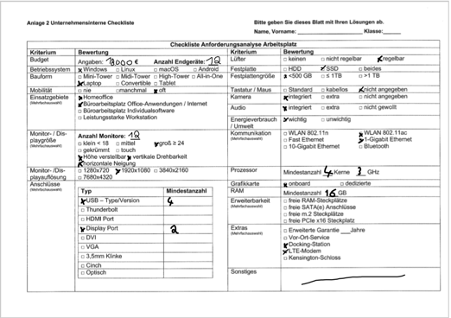
\includegraphics{solution.png}
\end{figure}

\end{flushleft}
\end{document}
